% Options for packages loaded elsewhere
\PassOptionsToPackage{unicode}{hyperref}
\PassOptionsToPackage{hyphens}{url}
\PassOptionsToPackage{dvipsnames,svgnames,x11names}{xcolor}
\documentclass[
  11pt,
  oneside,
  fontset=fandol]{ctexbook}
\usepackage{xcolor}
\usepackage[margin=25mm]{geometry}
\usepackage{amsmath,amssymb}
\setcounter{secnumdepth}{-\maxdimen} % remove section numbering
\usepackage{iftex}
\usepackage[most]{tcolorbox}
\definecolor{customgreen}{HTML}{01C260}
\ifPDFTeX
  \usepackage[T1]{fontenc}
  \usepackage[utf8]{inputenc}
  \usepackage{textcomp} % provide euro and other symbols
\else % if luatex or xetex
  \usepackage{unicode-math} % this also loads fontspec
  \defaultfontfeatures{Scale=MatchLowercase}
  \defaultfontfeatures[\rmfamily]{Ligatures=TeX,Scale=1}
\fi
\usepackage{lmodern}
\ifPDFTeX\else
  % xetex/luatex font selection
  % Load TeX Live font files directly, independent of macOS font registration.
  \setmainfont{texgyretermes}[
    Extension=.otf,
    UprightFont=*-regular,
    BoldFont=*-bold,
    ItalicFont=*-italic,
    BoldItalicFont=*-bolditalic]
  \setsansfont{texgyreheros}[
    Extension=.otf,
    UprightFont=*-regular,
    BoldFont=*-bold,
    ItalicFont=*-italic,
    BoldItalicFont=*-bolditalic]
  \setmonofont{lmmono10}[
    Extension=.otf,
    UprightFont=*-regular,
    ItalicFont=*-italic,
    BoldFont=lmmonolt10-bold,
    BoldItalicFont=lmmonolt10-boldoblique]
\fi
% Use upquote if available, for straight quotes in verbatim environments
\IfFileExists{upquote.sty}{\usepackage{upquote}}{}
\IfFileExists{microtype.sty}{% use microtype if available
  \usepackage[]{microtype}
  \UseMicrotypeSet[protrusion]{basicmath} % disable protrusion for tt fonts
}{}
\makeatletter
\@ifundefined{KOMAClassName}{% if non-KOMA class
  \IfFileExists{parskip.sty}{%
    \usepackage{parskip}
  }{% else
    \setlength{\parindent}{0pt}
    \setlength{\parskip}{6pt plus 2pt minus 1pt}}
}{% if KOMA class
  \KOMAoptions{parskip=half}}
\makeatother
\usepackage{longtable,booktabs,array}
\usepackage{calc} % for calculating minipage widths
% Correct order of tables after \paragraph or \subparagraph
\usepackage{etoolbox}
\makeatletter
\patchcmd\longtable{\par}{\if@noskipsec\mbox{}\fi\par}{}{}
\makeatother
% Allow footnotes in longtable head/foot
\IfFileExists{footnotehyper.sty}{\usepackage{footnotehyper}}{\usepackage{footnote}}
\makesavenoteenv{longtable}
\usepackage{graphicx}
\makeatletter
\newsavebox\pandoc@box
\newcommand*\pandocbounded[1]{% scales image to fit in text height/width
  \sbox\pandoc@box{#1}%
  \Gscale@div\@tempa{\textheight}{\dimexpr\ht\pandoc@box+\dp\pandoc@box\relax}%
  \Gscale@div\@tempb{\linewidth}{\wd\pandoc@box}%
  \ifdim\@tempb\p@<\@tempa\p@\let\@tempa\@tempb\fi% select the smaller of both
  \ifdim\@tempa\p@<\p@\scalebox{\@tempa}{\usebox\pandoc@box}%
  \else\usebox{\pandoc@box}%
  \fi%
}
% Set default figure placement to htbp
\def\fps@figure{htbp}
\makeatother
\setlength{\emergencystretch}{3em} % prevent overfull lines
\providecommand{\tightlist}{%
  \setlength{\itemsep}{0pt}\setlength{\parskip}{0pt}}
% Shared layout settings. UTF-8 source; compile with XeLaTeX.
\usepackage{microtype}
\usepackage{xurl}
\setcounter{tocdepth}{1}
\setcounter{secnumdepth}{1}
\setlength{\emergencystretch}{3em}
\setlength{\parskip}{0.35em}
\ctexset{chapter={format=\huge\bfseries},section={format=\Large\bfseries}}
\AtBeginEnvironment{longtable}{\small}

\usepackage{bookmark}
\IfFileExists{xurl.sty}{\usepackage{xurl}}{} % add URL line breaks if available
\urlstyle{same}
\hypersetup{
  pdftitle={大模型入门教材},
  colorlinks=true,
  linkcolor={black},
  filecolor={Maroon},
  citecolor={Blue},
  urlcolor={blue},
  pdfcreator={LaTeX via pandoc}}

\title{大模型入门教材}
\usepackage{etoolbox}
\makeatletter
\providecommand{\subtitle}[1]{% add subtitle to \maketitle
  \apptocmd{\@title}{\par {\large #1 \par}}{}{}
}
\makeatother
\subtitle{训练一个可靠的学习助手}
\author{}
\date{}

\begin{document}
\hypersetup{pageanchor=false}
\begin{titlepage}
\centering
\vspace*{0.2\textheight}
{\Huge\bfseries 大模型入门教材\par}
\vspace{1.5em}
{\Large 训练一个可靠的学习助手\par}
\vspace{3em}
面向具备基础编程能力的大模型初学者

最后修订日期 2026 年 10 月 25 日

李孙博闻~北京理工大学

\vfill
\end{titlepage}
\hypersetup{pageanchor=true}
\frontmatter



\chapter{写在开始之前}\label{写在开始之前}

这本教材邀请我们共同完成一件事：把一个善于续写文本的大语言模型（Large Language Model，LLM），逐步变成能讲题、能查资料、能使用工具，也能承认信息不足的学习助手。我们暂时叫它``小助''。名字只是为了叙述方便。

我们会保留一条清楚的故事线。起初，小助连``请回答问题''都不总能做到。我们用案例示范教它回答，它才开始像一个助手，却会在续训新课程资料后丢掉原来的讲解习惯。我们让它多试几次，发现偶尔能答对，于是尝试筛选和强化学习。分数开始上涨，我们又发现验证集没有进步。最后，我们把检索、工具和评估接入系统，才意识到：可靠的助手来自模型、数据、训练与应用共同作用。

我们默认自己会写基本程序，知道数组和函数的含义。正文首次引入术语时给出中文名、英文全称与常用缩写，后文沿用；模型名和论文题名保留原名或给出代称。遇到概率、向量、梯度时，正文会就地补上够用的数学。初读时，我们先追踪``问题为什么出现、证据支持什么、下一步如何验证''；第二遍再推公式和复现实验。全书按九部分展开，适合约八到十二周的学习，也可以按课堂节奏拆分。每个编号小节都包含完整讲解，以及关键论文与补充材料的阅读入口。

书中``小助''的回答、行为和数值案例均为教学构造，用来练习推理与诊断。在实际实验或者工程任务中，则需要记录模型版本、数据划分、模板、随机种子、计算预算与解码配置。

本材料一到三章希望构建一个对大模型的基本理解，包括tokenizer，词嵌入，句子嵌入，并且把大模型的行为理解为 next token prediction的条件分布。四到六章串讲现代大模型全部训练方法。后续章节则尽量对大模型各个方向做一个入门性质的学习。

任何方法都不保证在所有模型和任务上有效；我们关心的是如何识别和理解任务中的有效条件。本教材尽可能不堆砌概念和知识点逐一介绍，而是尽可能拉通每个部分，希望读者能够自然地理解从上一步到下一步的逻辑关系，这样有助于理解整个大模型体系。本教材省略了许多技术细节，这些技术细节是成为大模型专家不可或缺的一部分，如果读者立志成为该领域的专家，建议读者自学 Hugging Face 大语言模型课程与 Stanford CS336《从零构建语言模型》的视频和材料。

实际上，在当前的科研甚至工业研发场景下，本教材所提到的许多知识可能永远都用不上，例如一名后训练算法工程师通常只需要掌握数据合成、后训练方法（最基础的SFT和RL）就可以完成大部分工作，甚至不需要关心词表、嵌入层等模型架构的知识，一名大模型工程师真正重要的能力在于碰到问题时能够有思路去摸索和解决问题，这就要求我们有尽可能准确和发散的思维，有科学可复用的方法论指导实践。

\tableofcontents
\mainmatter
\chapter{定义一个值得训练的助手}\label{定义一个值得训练的助手}

\section{任务定义与评估 从一次失败开始}\label{任务定义与评估 从一次失败开始}

我们把一道题交给小助：``请解方程 3(a＋2)＝21，并解释每一步。''我们期待它先除以 3，再减去 2，得到 a＝5。它却接着写：``这是初中代数教材中的一道基础题，下面还有几道同类练习。''句子很通顺，也与题目有关，但它没有完成任务。

\emph{我们容易把这次失败归结为``模型不够聪明''。可如果把提示改成一段问答示例，再把同一道题放在末尾，它也许就能给出正确答案。}此时，算力和参数都没变，变化的是上下文。这提醒我们，至少要区分三个问题：模型能否表示所需知识；在当前提示下会生成什么；模型是否把这种生成转成了用户需要的行为。

基座语言模型学习的是文本延续规律。真实语料里，问题后面可能跟答案，也可能跟题目分析、引用、另一道题，甚至空白。我们给了一个任务，小助并不会自动地将这个任务作为唯一目标，因为它还不知道问题和回答之间的区别，哪里是问题的开始，哪里是问题的结束，哪里是回答的开始等。

在训练之前，我们通常先写一份小型验收约定。我们选出四类需求：讲清基础题；回答课程资料问题；在缺少资料时说不确定；通过计算器处理容易算错的数值。我们把``正确率''和``讲解质量''分开，把``引用存在''和``引用支持结论''分开。一个回答可以结果正确但过程错误，也可以格式漂亮却没有逻辑依据。

和传统机器学习一样，我们通常准备三份数据。训练集用来更新参数；验证集用来选提示、超参和检查点；最终测试集留到方案确定后使用。以后若反复根据同一份验证集修改方案，它事实上已经参与了开发，不能继续被当成完全独立的泛化证明。同一道母题的改写也应成组划分，避免训练和评估只是换了姓名与数字。当然，这是传统机器学习的思路，许多大模型的工程实践中基本没有验证集，研发人员直接合成训练数据并且在测试集上测试效果并且根据结果反馈调整训练集，尽管这是不够严谨的。

从这一步起，我们把``效果好像变好了''细化为成可核验的问题：哪类任务改善了，哪类退步了，在相同预算下是否仍成立？这份最初的评估约定，会在监督微调（Supervised Fine-Tuning，SFT）续训和强化学习（Reinforcement Learning，RL）过程中遇到麻烦时成为我们的定位工具。SFT 用示范回答训练模型，RL 则依据反馈优化模型的尝试；我们稍后会逐步展开。

\textbf{探索问题}~如何解释对于预训练模型：``\emph{我们容易把这次失败归结为``模型不够聪明''。可如果把提示改成一段问答示例，再把同一道题放在末尾，它也许就能给出正确答案。''}这个现象。

\textbf{本节相关资料}
\begin{enumerate}
    \item Brown 等，2020，\href{https://arxiv.org/abs/2005.14165}{Language Models are Few-Shot Learners} 。阅读重点：同一个模型为什么能通过上下文示例切换任务。
\end{enumerate}

\section{训练阶段 语言学习类比能解释什么}\label{训练阶段 语言学习类比能解释什么}

为了理解接下来发生的事，我们先想象一个熟悉的过程。婴儿长期听到周围的人说话，逐渐熟悉声音与表达；后来在互动中练习表达，得到示范和反馈。这能帮助我们建立一个入口：大量接触语言、学习具体表达、再依据结果调整，是彼此衔接但不相同的学习环节。

我们可以把预训练类比为广泛接触语言，把监督微调类比为有人示范``面对这个问题，可以这样回答''，把反馈学习类比为比较不同回答是否合适。这个类比让抽象的训练阶段有了生活背景，但仍然有一点区别：模型不会经历人类婴儿的发育过程。

婴儿有身体、感知、共同注意和社会互动。文本语言模型的预训练通常是在已有序列上预测下一个词元（token，即分词后的基本处理单元），并通过误差更新参数。注意，当我们提到大模型的行为时，经常指代的就是模型的``分布''。它在预训练时已经反复``尝试预测''，并非只听不说；SFT 也常使用同一种逐 token 交叉熵（cross-entropy）损失，并不是第一次获得生成能力。两者的重要区别在于数据的组织、监督的位置和我们希望强化的行为分布\footnote{理解大模型的输出（行为）是基于概率分布的，即根据上下文，从下一个token的概率分布中采样}。

预训练已经初步确定了 next token 分布，所以后训练叫做微调。不过因为注意力机制的存在，实际分布由参数和上下文共同决定，所以对于一个问题，后续解答时next token 分布不仅由问题本身决定，也跟其他上下文有关，比如问题前面可能还有一个解题指导，有指导地解题和无指导地解题难度肯定是不一样的，所以分布也有差异。全量后训练通常会训练大量数据，这样也可以比较明显改变模型的分布，这种规模的训练就不再是``微调''了。我们还可以做小规模后训练，比如在别人已经训练好的模型上继续用比较少的数据做SFT或者RL训练，这种小规模后训练的能力范围受训练起点、数据、优化与预算限制，通常很难大幅度调整模型的行为，甚至可能导致模型的通用能力收到影响。类似于一个人在大学系统性学习了四年中国哲学，后来自学了几个月西方哲学，那么西哲主要是做了一点思想补充和调整，其主干思维可能还是以中哲为主。

不妨想象小助对一道题能给出三种回答。训练前，它有时直接给答案，有时续写题目，有时解释步骤。SFT 提高给出高质量解题流程的概率；RL 依据奖励重新分配不同尝试的概率，比如同一个题目可能有好几种解题方案，可以通过给更好的解题方案更高的奖励来使得模型更倾向于生成这种更好的解题方案，这是一种偏好调整。若它从未形成某个关键运算过程，单靠稀疏奖励去生成完整解法可能很困难；若它已经偶尔做对，强化学习的奖励就可能帮助它更稳定地选到有效路径，比如解题 10 次，只对了2次，我们奖励这两次形成的解题轨迹，模型就会在这类问题上更倾向于走这条轨迹。

因此，这本书中的``学会''和``知道''都是方便交流的简写。落实到实验，我们总会追问：在哪些输入、怎样的解码条件和多少预算下，模型表现出了什么行为？有了这层约定，我们就能借助故事建立直觉，同时用机制纠正直觉。

\textbf{实践}~查资料或者实践看一下预训练数据和后训练数据有什么区别。

\textbf{本节相关资料}
\begin{enumerate}
    \item Ouyang 等，2022，\href{https://arxiv.org/abs/2203.02155}{Training language models to follow instructions with human feedback}，也就是 InstructGPT。阅读重点：如何利用人类反馈来优化大模型的行为。\textbf{该文章是人类偏好强化学习（RLHF）的里程碑论文之一，可以提前阅读，也可以在学到强化学习时阅读。}
\end{enumerate}


\chapter{语言模型与文本预测}\label{语言模型与文本预测}

\section{分词器 Tokenizer 模型看到的是什么}\label{分词器 Tokenizer 模型看到的是什么}

我们决定先观察小助的输入。屏幕上是一段中文题目，进入模型的却是一串整数。这些整数不是天然对应每个汉字，也不一定对应一个完整单词；它们是分词器（tokenizer）按词表规则把文本切分后得到的词元标识符（token identifier，token ID）；后文沿用 token 和 token ID。

我们用一个极小例子理解子词分词。若词表保存完整英文单词，遇到从未见过的复合词就很难处理；若只保存字符，序列又会变长。字节对编码（Byte Pair Encoding，BPE）一类方法从小单元出发，逐步合并常见相邻片段，在词表大小与序列长度之间折中。实际 tokenizer 还有字节回退、预处理和特殊标记等差异。

一个经典的例子：我们输入 strawberry，想让小助数出字母 r 的个数。人眼可以直接扫描字符；模型可能看到几个子词片段（比如 staw 和 berry 两个 token，而不是 s t r a w\ldots 这样把每个字母都切分开），模型就需要把片段重新关联到字符，再执行计数，比如模型可能知道berry 这个 token 和字母 r 是有关系的，然后就会思考berry这个 token 由哪几个字母token 组成，模型能够做到这一点，可能是因为预训练数据中有一些关于单词拼写的语料，或者后训练中有专项训练。分词让任务的表示过程更绕，许多模型都会数错，但不能断言模型一定数错：模型可以通过训练、内部计算或外部工具完成任务。这个例子说明的是输入文本的粒度与模型理解的任务粒度是不同的。

对话还有一层常被忽略的编码。我们在界面里看见 系统（system）、用户（user）、助手（assistant）三种角色，模型实际接收的通常是由对话模板（chat template）拼成的序列，其中含有角色边界、轮次结束和生成起点等标记。角色名称可能是普通文本与特殊 token 的组合，不是所有模板都把每个角色名设为一个特殊 token。建议在AI的帮助下看一些实际案例，理解模型如何切分或组合文本为token。

当我们问问题的时候，大模型看到的内容及其完整回答里面有许多标记，自然语言夹杂在这些标记中间，这些标记是为了方便机器区分不同的文本对话。我们问：``洗车店在 50 米外，我要洗车，是开车去还是步行过去''，许多模型会给出错误的回答，比如走过去，实际上洗车就必须开车去。下面是一个模型所看到的完整序列：

我们拆解一下具体过程：

\begin{tcolorbox}[colback=gray!10, colframe=customgreen, title=对话原始文本, arc=4mm]
\textless\textbar im\_start\textbar\textgreater\allowbreak{} user\textbackslash n\allowbreak{}洗车店在 50 米外，我要洗车，是开车去还是步行过去\textless\textbar im\_end\textbar\textgreater\allowbreak{}\textbackslash n\allowbreak{}\textless\textbar im\_start\textbar\textgreater\allowbreak{} assistant\textbackslash n\allowbreak{}\textless think\textgreater\allowbreak{} 用户问的是：洗车店在50米外，要洗车，是开车去还是步行过去。\textbackslash n\allowbreak{}\textbackslash n\allowbreak{}这是一个简单的生活常识/决策问题。50米非常近，大概就是步行几十秒的距离。开车反而可能更麻烦（找停车位、倒车入库等），而且50米开过去可能一个路口都没到就到了。\textbackslash n\allowbreak{}\textbackslash n\allowbreak{}我应该给出简短、明确的建议：步行过去。理由：50米很近，步行约一分钟，开车反而费事（找车位、倒车等）。\textless/think\textgreater\allowbreak{}50米太近了，**步行过去**最省事。\textbackslash n\allowbreak{}\textbackslash n\allowbreak{}- 步行也就**几十秒到一分钟**，一脚油门一踩就过了，根本不值得专门发动车子。\textbackslash n\allowbreak{}- 开车过去还得找停车位、倒车入库，搞不好比走路还费劲。\textbackslash n\allowbreak{}- 还省了点油耗和停车费。\textbackslash n\allowbreak{}\textbackslash n\allowbreak{}所以锁好车，走过去就行，到了直接把钥匙交给店员。\textless\textbar im\_end\textbar\textgreater\allowbreak{}{}
\end{tcolorbox}

首先我们发送了一个问题，那么此时一定是对话的开始，所以自动在开头以 ``\textless\textbar im\_start\textbar\textgreater\allowbreak{} user\textbackslash n\allowbreak{}''开始，表示用户问题开始，然后拼上我们的问题，在问题结束以后自动拼上``\textless\textbar im\_end\textbar\textgreater\allowbreak{}\textbackslash n\allowbreak{}''，表示用户问题结束，接下来需要加上标记让模型知道轮到它生成，类似前面的标记，拼上``\textless\textbar im\_start\textbar\textgreater\allowbreak{} assistant\textbackslash n\allowbreak{}''，并且我们要求模型必须先思考再回答，所以加上``\textless think\textgreater\allowbreak{}''，那么模型在自己生成之前，看到的内容就是前面这些，接下来模型就自己生成一段思考内容，模型自己决定在哪里结束，在适当的位置自己拼上``\textless/think\textgreater\allowbreak{}''结束思考，接下来就是面向用户的总结回答，回答结束，模型自己拼上``\textless\textbar im\_end\textbar\textgreater\allowbreak{}''，这就是一个完整的生成过程。

图\ref{fig:对话案例}是一个比较清晰的图例，去掉标记符拆分了上面的原始文本。

\begin{figure}[t]
    \centering
    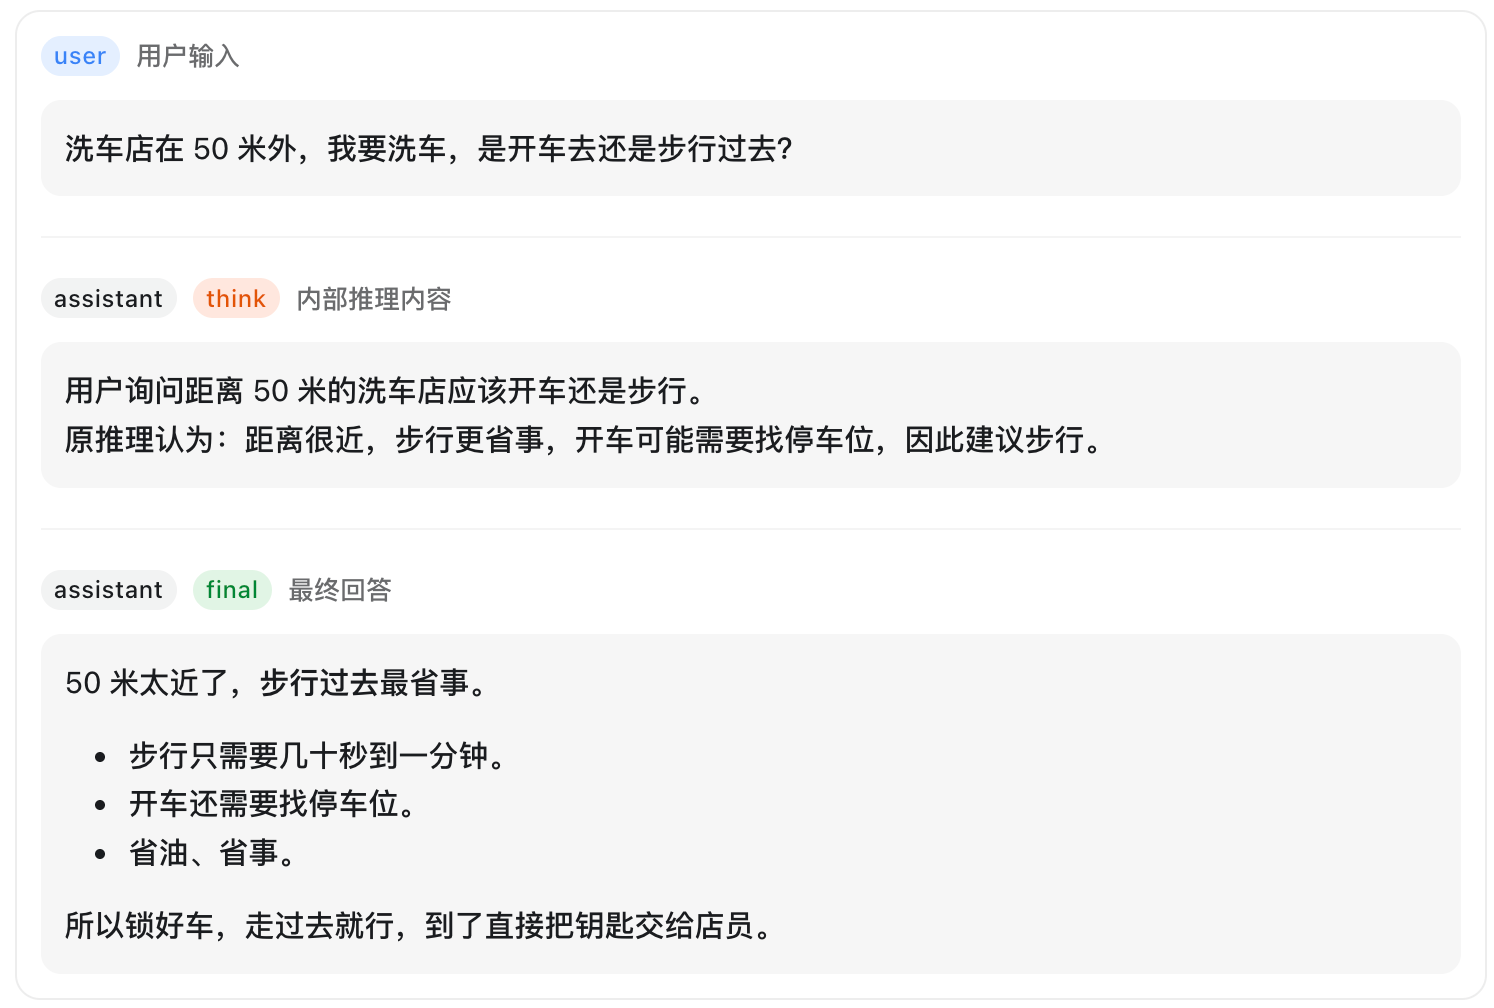
\includegraphics[width=\linewidth]{assets/media/image1.png}
    \caption{对话案例}
    \label{fig:对话案例}
\end{figure}

为什么这些标记有效，以及为什么大模型认识这些标记？模型在预训练的时候是不会见到这些标记的，但是在后训练的时候会接受大量带有这些标记的数据训练，训练之后，模型的行为分布就会变成这样，比如，不管上下文是什么，在 \textless think\textgreater\allowbreak{}{} 之后一定是思考的内容，思考完毕一定要生成一个 \textless/think\textgreater\allowbreak{}\textbackslash n\allowbreak{}\textbackslash n\allowbreak{}，然后才是给用户的回答，所以当我们要求模型进行思考时，就在模型开始推理之前拼上\textless think\textgreater\allowbreak{}，如果我们问的是一个很简单的问题，不希望模型思考，只是要模型快速回答，那么就在开始推理之前拼上\textless think\textgreater\allowbreak{}\textless/think\textgreater\allowbreak{}\textbackslash n\allowbreak{}\textbackslash n\allowbreak{}，模型就知道现在不需要思考，直接给出最终回答。我们与大模型对话的时候有一个思考开关，这个开关控制的就是这个 think 标签如何拼接在模型回答的开头。但是这个行为也是训练的概率分布，既然是概率分布就会有小概率事件，许多模型可能在 1\% 的案例中缺少 \textless/think\textgreater\allowbreak{}{} 标签或者出现其他格式错误，可能进一步造成前端显示错误。

假如训练时回答前有起始标记，推理时却漏掉起始标记，小助可能把用户内容（问题）继续写下去。假如停止标记 \textless\textbar im\_end\textbar\textgreater\allowbreak{}{} 配置错了，它可能回答完以后继续模拟用户提问，因为他不知道回答结束了，会继续写下去（因为预训练的时候问答语料可能就是这样的，在答案后面跟着下一个问题）。还有思考标记 \textless think\textgreater\allowbreak{} 也可能出问题 ，在真实工程中，有些模型的 \textless think\textgreater\allowbreak{}{} 后面一般还必须跟着两个回车（\textbackslash n\allowbreak{}\textbackslash n\allowbreak{}），如果我们的模板错了，没有这两个回车，模型的表现会打折扣，原本在一个榜单上可以做到 90分，但是因为模板错误，少了两个回车，可能就只有 85分（这种分数不一致的情况称为精度错误，其原因可能是模板错，可能是模型配置错，甚至可能和推理框架的bug有关）\textbf{。}一般来说，think 和工具等标记可能由模型自己生成，其他的标记可以由脚本自动生成，比如在模型的权重目录中有一个 chat\_template.jinja 文件来自动处理标记，这个功能也可能集成到其他的配置文件中，建议读者在huggingface或者modelscope网站中找到一些常用的开源模型，看看这些模型的文件构成。

序列长度还决定成本。同一份资料在不同 tokenizer 下可能占用不同数量的 token，因为分词规则不同；长序列会影响训练显存、截断位置、推理延迟和可用上下文。因此，``字符数''与``token数''不能互换，模型的序列长度计数是基于token的。

我们还要区分``切分有错''和``某个 token 难以生成''。MiniMax 在 2026 年公布的``马嘉祺''案例中，人们发现 Minimax M3 模型知道``马嘉祺''是谁，但是无法输出``马嘉祺''三个字。他们的研究案例提醒我们：一个词生成不出来，不足以证明 tokenizer 损坏。MiniMax 的研究者对这个问题进行了非常有参考价值的探索研究并且写成\href{https://www.minimax.cn/blog/sparse-token-forgetting-investigation}{博客}\footnote{https://www.minimax.cn/blog/sparse-token-forgetting-investigation}。

\textbf{实践} 在 OpenAI 的\href{https://platform.openai.com/tokenizer?utm_source=chatgpt.com}{分词器网站}\footnote{https://platform.openai.com/tokenizer?utm\_source=chatgpt.com}里面尝试各种文本，看看大模型是如何分词的。

\textbf{本节相关资料}
\begin{enumerate}
    \item Touvron 等，2023，\href{https://arxiv.org/abs/2307.09288}{Llama 2 Open Foundation and Fine-Tuned Chat Models} 。阅读重点：对话训练与模型使用约定如何共同影响行为。
    \item \textbf{（建议阅读）MiniMax Research，2026，\href{https://www.minimax.cn/blog/sparse-token-forgetting-investigation}{为什么 MiniMax 大模型不认识``马嘉祺'' 稀疏 Token 遗忘排查记录研究博客} 。阅读重点：如何先排除分词不一致，再检查后训练变化；与第 4.3 节对照阅读，搞清楚这个问题还需要对大模型结构有了解，比如LM head。}
\end{enumerate}

\section{下一个词元预测 NTP 从损失到信息压缩}\label{下一个词元预测 NTP 从损失到信息压缩}

本节内容对初学者来说可能比较抽象，观看 1Blue3Brown 的 \href{https://www.bilibili.com/video/BV1yVNU6xERx}{{信息压缩}}\footnote{https://www.bilibili.com/video/BV1yVNU6xERx} 视频解说可以替代本节学习。最主要的是理解这样一个观点：大模型训练可以视为信息压缩。

现在我们把小助暂时简化成一个函数：输入此前的 token，输出词表上所有候选 token 的概率。对``法国的首都是''这个前缀，它可能给``巴黎''相关的首个 token 较高概率，也给其他延续保留概率。生成时，我们从这些概率中选一个 token，接回前缀，再重复同样的过程。

这就是下一个词元预测（Next Token Prediction，NTP）。给定此前的 token，模型对下一个位置给出一个条件概率分布：
\[p_{\theta}\left( x_{t} \mid x_{< t} \right) = p_{\theta}\left( x_{t} \mid x_{1},\ldots,x_{t - 1} \right)\]

这里 θ 表示模型参数，t 表示位置，x 的下标表示序列中的 token，x 的下标小于 t 表示此前的完整前缀。对词表中所有可能的下一个 token，这些概率加起来为 1。我们不是先生成一句完整答案再给它评分，而是一步步预测。

若整段文本有 T 个 token，把这些条件概率相乘就得到序列概率。按照概率链式法则，自回归分解写为：
\[p_{\theta}\left( x_{1:T} \right) = \prod_{t = 1}^{T}p_{\theta}\left( x_{t} \mid x_{< t} \right)\]

上式中，x 的下标 1 到 T 表示整段序列，T 是序列长度，乘积号表示把各位置的条件概率相乘。每个位置都贡献一个预测任务，因此一段普通文本就能产生大量监督信号，不必另外给每个句子标上``语法课''或``事实课''。

怎样惩罚预测错误？我们取真实下一个 token 的概率，再取负对数。给正确 token 的概率越低，损失越大。若概率从 0.1 提高到 0.5，单个位置的负对数损失会从约 2.30 降到约 0.69。训练把大量位置的损失加总或平均，再用梯度更新参数。 把长度为 T 的序列在各位置的负对数概率取平均，NTP 损失写为：
\[L_{NTP} = - \frac{1}{T}\sum_{t = 1}^{T}\log p_{\theta}\left( x_{t} \mid x_{< t} \right)\]

这里 log 使用自然对数，损失的单位为 nat（奈特，自然对数的信息单位）；负号使低概率对应较大损失，前面的 1 除以 T 用来平均各位置。

为什么这个简单目标会与知识和推理有关？如果文本里出现``把 21 平均分成 3 份，每份是''，准确预测后续往往依赖算术关系；如果出现人物代词，预测可能依赖前文指代。模型可以利用词频捷径，也可能形成更可迁移的内部表示。目标并不逐条规定它必须怎样表示世界，我们要用新任务检验它究竟学到了什么。

在分布层面，交叉熵可以拆成真实数据分布的熵与一个\textbf{库尔贝克与莱布勒散度（Kullback--Leibler Divergence，KL 散度）}\footnote{KL散度是现代大模型技术中的高频概念，建议自行补充学习}。真实分布不随模型参数改变，因此最小化理想的总体交叉熵，等价于最小化数据分布到模型分布的正向 KL。有限训练集上的经验损失只是这个总体目标的估计，不能保证覆盖未见过的输入。 设 p 是真实数据分布、q 是模型分布，交叉熵与 KL 的关系具体写为：
\[H(p,q) = H(p) + D_{KL}\left( p\| q \right)\]

\(H(p,q)\) 是交叉熵，\(H(p)\) 是数据自身的熵，D 的下标 KL 表示从 p 到 q 的分布差异。p 固定时，H(p) 不随参数变化，因此优化交叉熵与优化这一 KL 项具有相同的方向。

我们已经知道，给真实 token 更高概率会降低损失。可是，为什么有人又把这说成``更会压缩''？先不急着看区间表，我们让小助承担一个具体任务：把课程文本存进文件，再从文件中逐字还原。这里讨论的是无损压缩（lossless compression），目标是在不丢失原序列的前提下减少比特数；写摘要、删掉重复句、只保留大意，都没有满足这个目标。

\textbf{先明确我们究竟在省什么} 假设消息只含 A 和 B，两者各用一个二进制位表示，100 个符号就要 100 bit。真实文本通常先由字符编码表示成字节，基线并非``一字一 bit''；我们先用二符号信源，是为了把统计结构与文本编码的细节分开。压缩器最终存下的是比特流，不是一段更短但意思差不多的自然语言。

编码器看到了原消息，解码器没有看到。两端要约定符号顺序、概率模型和消息如何结束，解码器才能从比特流唯一恢复原消息。若必须把新词表、概率表或模型权重一并发送，这些也属于总成本；只报``正文编码用了多少位''会夸大节省量。图 \ref{fig:无损压缩} 先把这份通信约定画出来：

\begin{figure}[t]
    \centering
    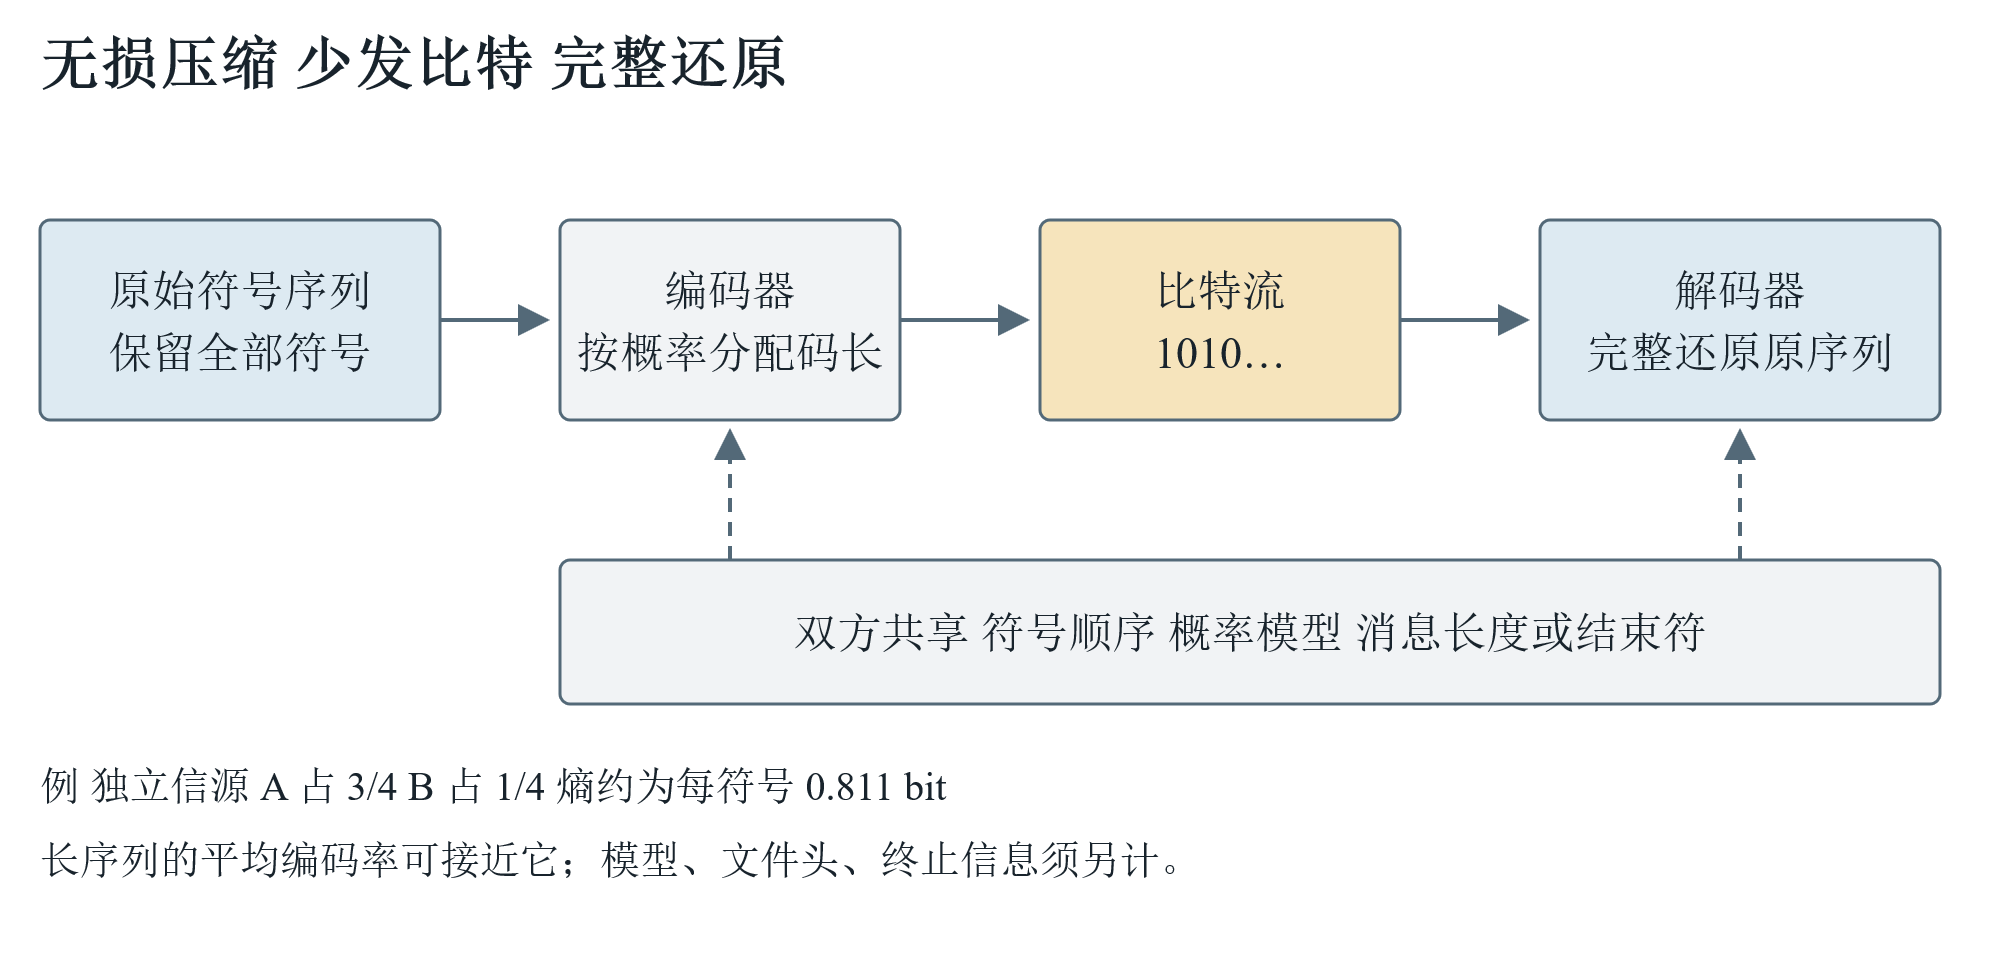
\includegraphics[width=\linewidth]{assets/media/image2.png}
    \caption{无损压缩的目标与两端约定。发送的是足以唯一定位原消息的比特流，接收端必须还原同一条符号序列。}
    \label{fig:无损压缩}
\end{figure}

\textbf{为什么概率能够帮助省位数} 在可唯一解码的约束下，我们不能给每条消息都分配更短的码：短二进制串的数量有限。统计压缩把较短的表示优先留给常见消息，让不常见的消息承担较长的表示，从而降低平均成本。因此，压缩器可能让个别输入变长，尤其是很短或接近随机的输入；无损压缩不承诺每一个文件都缩小。

例如，若符号独立产生且 A 的概率为 3/4、B 为 1/4，我们可以把许多符号一起编码，长消息的平均每符号码率能够接近 0.811 bit，而固定表示是每符号 1 bit。这里比较的是指定信源下的长期平均量；实际有限文件还有终止、对齐和元数据开销。若 A、B 各占一半且彼此独立，就没有这份频率偏斜可利用；如果它们有上下文依赖，仍可以由条件模型进一步利用。

\textbf{算术编码怎样把概率变成比特} 算术编码（arithmetic coding）让编码器与解码器按相同概率划分区间。我们先从 {[}0, 1) 出发，每读一个符号，就按概率切分当前区间，只保留实际符号对应的那一段。待整条消息处理完，编码器发送一段二进制前缀，只要它表示的整个小区间都落在目标区间内，解码器就能确定这条消息。

我们用固定概率走一遍：A 的概率为 0.75，B 为 0.25，消息为 ABA。第一次读 A，保留 {[}0, 0.75)；第二次读 B，保留当前区间最后四分之一，得到 {[}0.5625, 0.75)；第三次读 A，保留当前区间前四分之三，得到 {[}0.5625, 0.703125)。下面每行把上一行选中的区间放大，横轴的尺度随行改变，参考图 \ref{fig:算术编码}。

\begin{figure}[t]
    \centering
    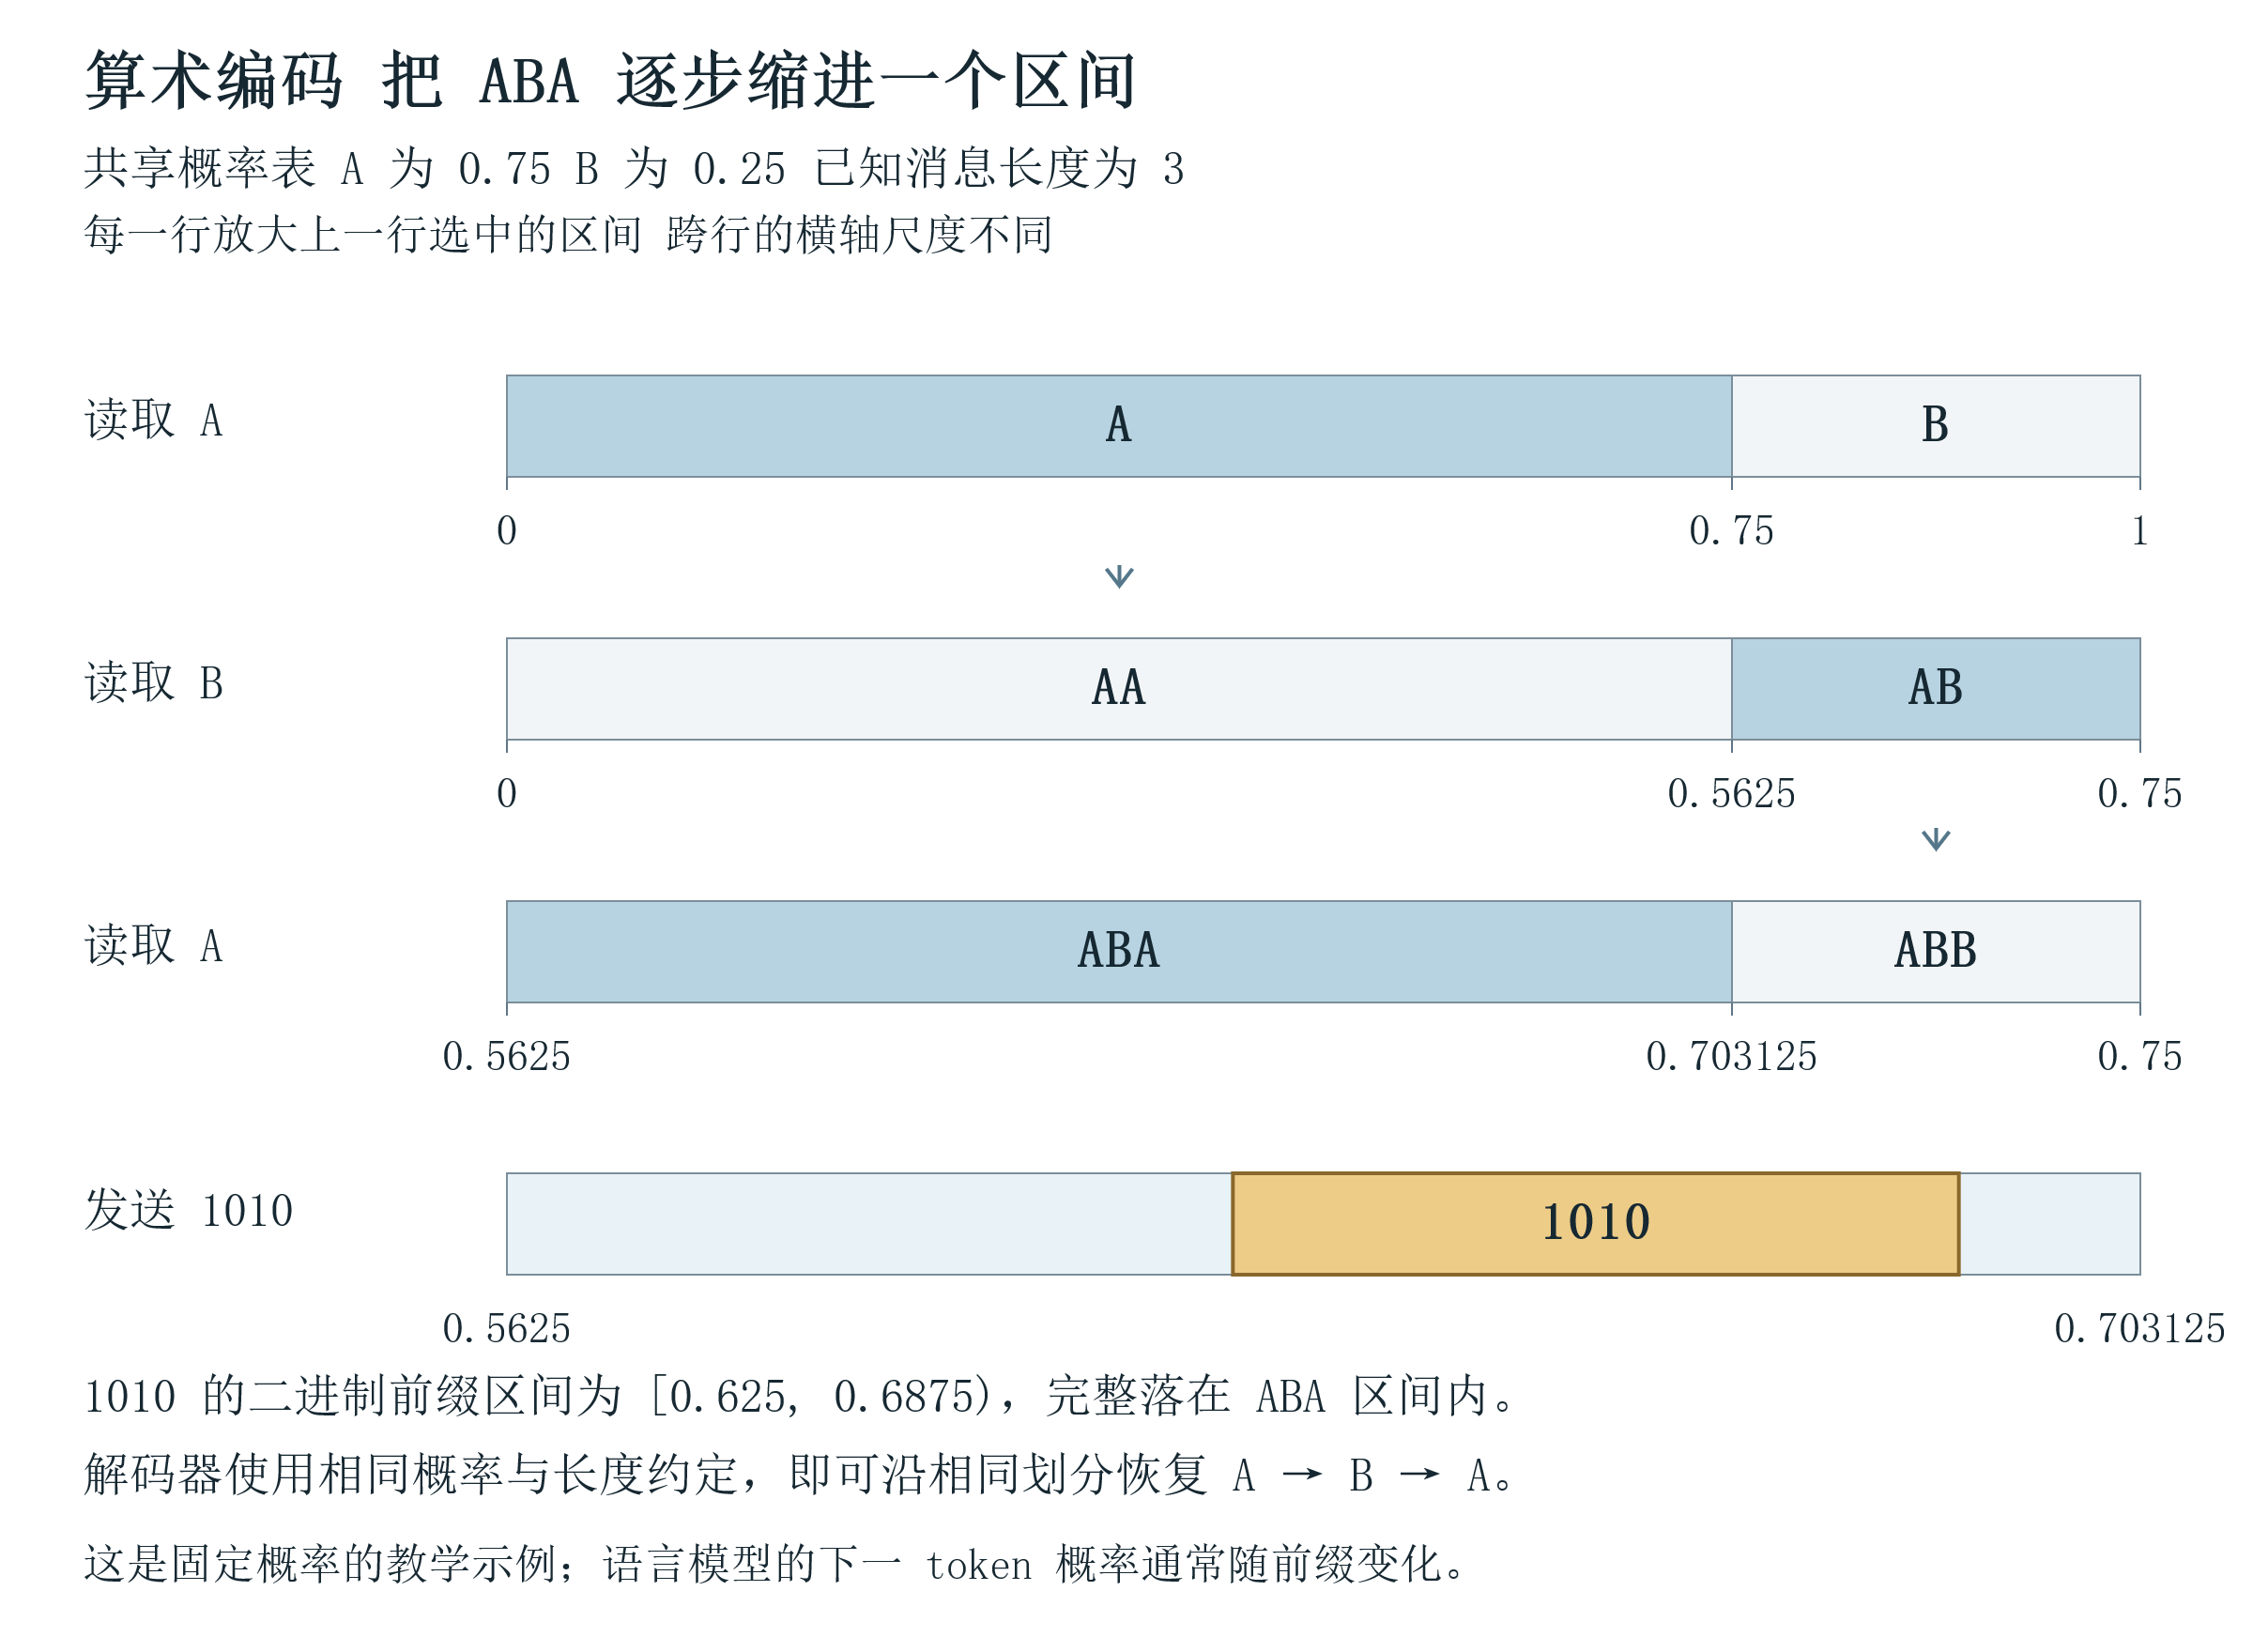
\includegraphics[width=\linewidth]{assets/media/image4.png}
    \caption{算术编码的区间细分。蓝色表示选中的符号区间，橙色表示发送的二进制前缀所对应的区间；跨行不能按图形长度比较绝对宽度。}
    \label{fig:算术编码}
\end{figure}

\textbf{1010 为什么足以还原 ABA} 二进制小数前缀 0.1010 的后续位尚未确定，因此它代表的全部数值位于 {[}0.625, 0.6875)。这个区间完整落在 ABA 的最终区间里。解码器可以取其中一个数，例如 0.625：它位于第一层的 A 区间；继续按同一概率细分，位于第二层的 AB 区间；再细分，位于第三层的 ABA 区间。双方已约定长度为 3，于是停止；若长度未知，就还需要结束符或其他长度协议。实际实现还要处理有限精度和逐步输出比特，我们这里先追踪数学上的区间。

这个例子发送了 4 bit，甚至比二符号固定表示 ABA 所需的 3 bit 更长。这并不矛盾：我们用极短消息展示了可逆机制，尚未展示长期平均压缩收益。若丢掉长度与模型开销、只看漂亮的区间图，就会把``能编码''误当成``这个样本一定更省''。

\textbf{码长怎样回到训练损失} 每选一次符号，区间宽度就乘上该符号的条件概率，所以最终宽度等于整串消息的模型概率。\(m\) 个二进制前缀位对应宽度为 2 的负 \(m\) 次方的区间。为了在目标区间内找到一个可用前缀，所需位数便与概率的以 2 为底负对数相联系。用 \(q\) 表示双方共享的编码模型、\(T\) 表示消息长度，理想信息量写为：
\[l_{q}\left( x_{1:T} \right) = - \log_{2}q\left( x_{1:T} \right) = - \sum_{t = 1}^{T}\log_{2}q\left( x_{t} \mid x_{< t} \right)\]

这里 ℓ 的单位是 bit，x 的下标 1 到 T 表示整串消息，右侧按位置相加；它是理想信息量，不是任意有限文件的最终整数位数。ABA 的概率是 0.75 × 0.25 × 0.75＝9/64，理想信息量约为 2.83 bit，而图中实际选用了 4 位前缀。

现在，前面的交叉熵也有了操作含义。假设真实消息服从 p，而我们按 q 分配码长，那么以 2 为底计算的交叉熵是理想编码长度的平均值；数据自身的熵描述信源不确定性，正向 KL 描述使用不匹配模型额外支付的平均长度。在同一数据上，把真实 token 的预测概率提高，会让对应的理想编码长度降低。

回到语言模型，我们可以让编码器与解码器共享同一个已训练模型。两端从相同起始状态开始；解码出一个 token 后，把它接回前缀，再算出相同的下一步概率。因此，解码器不需要提前知道原文，也不需要靠采样``猜''出原文，而是用收到的编码位从概率区间中确定原 token。两端的分词器、参数、数值实现与结束约定必须兼容。

前面的训练损失使用自然对数，单位为 nat；这里使用以 2 为底的对数，单位为 bit，除以 ln 2 即可把 nat 换成 bit。这个联系说明``预测更准为什么可能让编码更省''，却不表示常规推理会输出压缩文件，也不表示模型权重是训练文本的可逆压缩包，更不能仅据此断言模型已经理解每个事实或解决每道题。知识与推理能力仍要通过独立任务检验。

\section{Transformer 一次前向计算如何完成}\label{Transformer 一次前向计算如何完成}

如果觉得本节讲解过于简单抽象，可以自行查找相关视频学习，重点理解注意力计算、注意力掩码和位置编码ROPE。

知道目标还不够，我们还要知道小助怎样把前缀变成概率。最早的 n 元语法（n-gram）模型只统计有限窗口中的词组合，窗口一长，组合就迅速变稀疏。神经语言模型让上下文共享参数与表示，循环网络再把历史压进状态。变换器（Transformer）架构则让不同位置通过注意力直接交换信息，成为一条适合并行训练的路线。这个历史并非一条必然链，但能帮我们看见每种设计回应的困难。

我们先把 token ID 送入嵌入（embedding）层。它相当于一张可训练查找表：每个 ID 对应一个向量。向量本身没有天然的``第七维就是语法''含义；其意义来自训练后与其他参数的协同。位置编码提供顺序信息，否则模型难以区分``甲帮助乙''和``乙帮助甲''。其中，旋转位置嵌入（Rotary Position Embedding，RoPE）由苏剑林等人在 RoFormer 工作中提出：它按位置旋转查询向量与键向量的表示，让注意力分数能够体现相对位置关系。RoPE 的``相对''性质不等于可以无条件外推到任意长度。

进入一层注意力时，我们把这一层输入的每个位置表示排成矩阵 X。这里的 X 不是原始 token ID，而是已经进入模型计算的向量。同一个 X 分别乘上三套可训练投影矩阵，得到查询（query，Q）、键（key，K）和值（value，V）。它们来自同一批位置，但承担不同计算角色，不能把 Q、K、V 理解成输入中的三种不同词。

我们把三套投影矩阵记为 W 的下标 Q、K、V，投影关系写为：
\[Q = XW_{Q},\quad\quad K = XW_{K},\quad\quad V = XW_{V}\]

若 X 有 n 行，每行具有相同的输入隐藏维度，则查询与键投影把它映射到 d\ensuremath{{}_{k}} 维，值投影映射到 d\ensuremath{{}_{v}} 维；所以 Q、K 都有 n 行、d\ensuremath{{}_{k}} 列，V 有 n 行、d\ensuremath{{}_{v}} 列。这里省略投影偏置，并先讨论一个注意力头。下标用于标识投影角色，不表示它们要对不同的原文分别分词。

把所有位置的 query、key、value 分别排成矩阵 Q、K、V，缩放点积注意力的计算写为：
\[Attention(Q,K,V) = softmax\left( \frac{QK^{\top}}{\sqrt{d_{k}}} + M \right)V\]

上标转置符号表示转置；softmax 对每个 query 的候选 key 分数归一化，再用权重汇总 V。因果掩码 M 在可见位置取 0，在禁止关注的位置用负无穷屏蔽。

其中 d 的下标 k 表示每个 key 的维度；缩放有助于控制点积的数值范围。Q 与 K 的点积是在对应维度相乘后求和，表达一种可训练的匹配分数。M 是掩码。对我们讨论的因果语言模型，未来位置被遮住；训练时即使整段文本同时进入计算，也不能偷看尚未预测的 token。多头注意力让不同子空间并行建立关系。注意力权重是计算的一部分，不能直接当作完整的因果解释。

我们可以把 query 理解为``当前怎样匹配上下文''，key 理解为``每个位置提供怎样的匹配线索''，value 是最终被汇集的信息。这个类比只是计算角色的直觉，向量维度不必对应人类能命名的概念。图 \ref{fig:QKV计算} 把分数、权重和被加权的信息分开。

\begin{figure}[t]
    \centering
    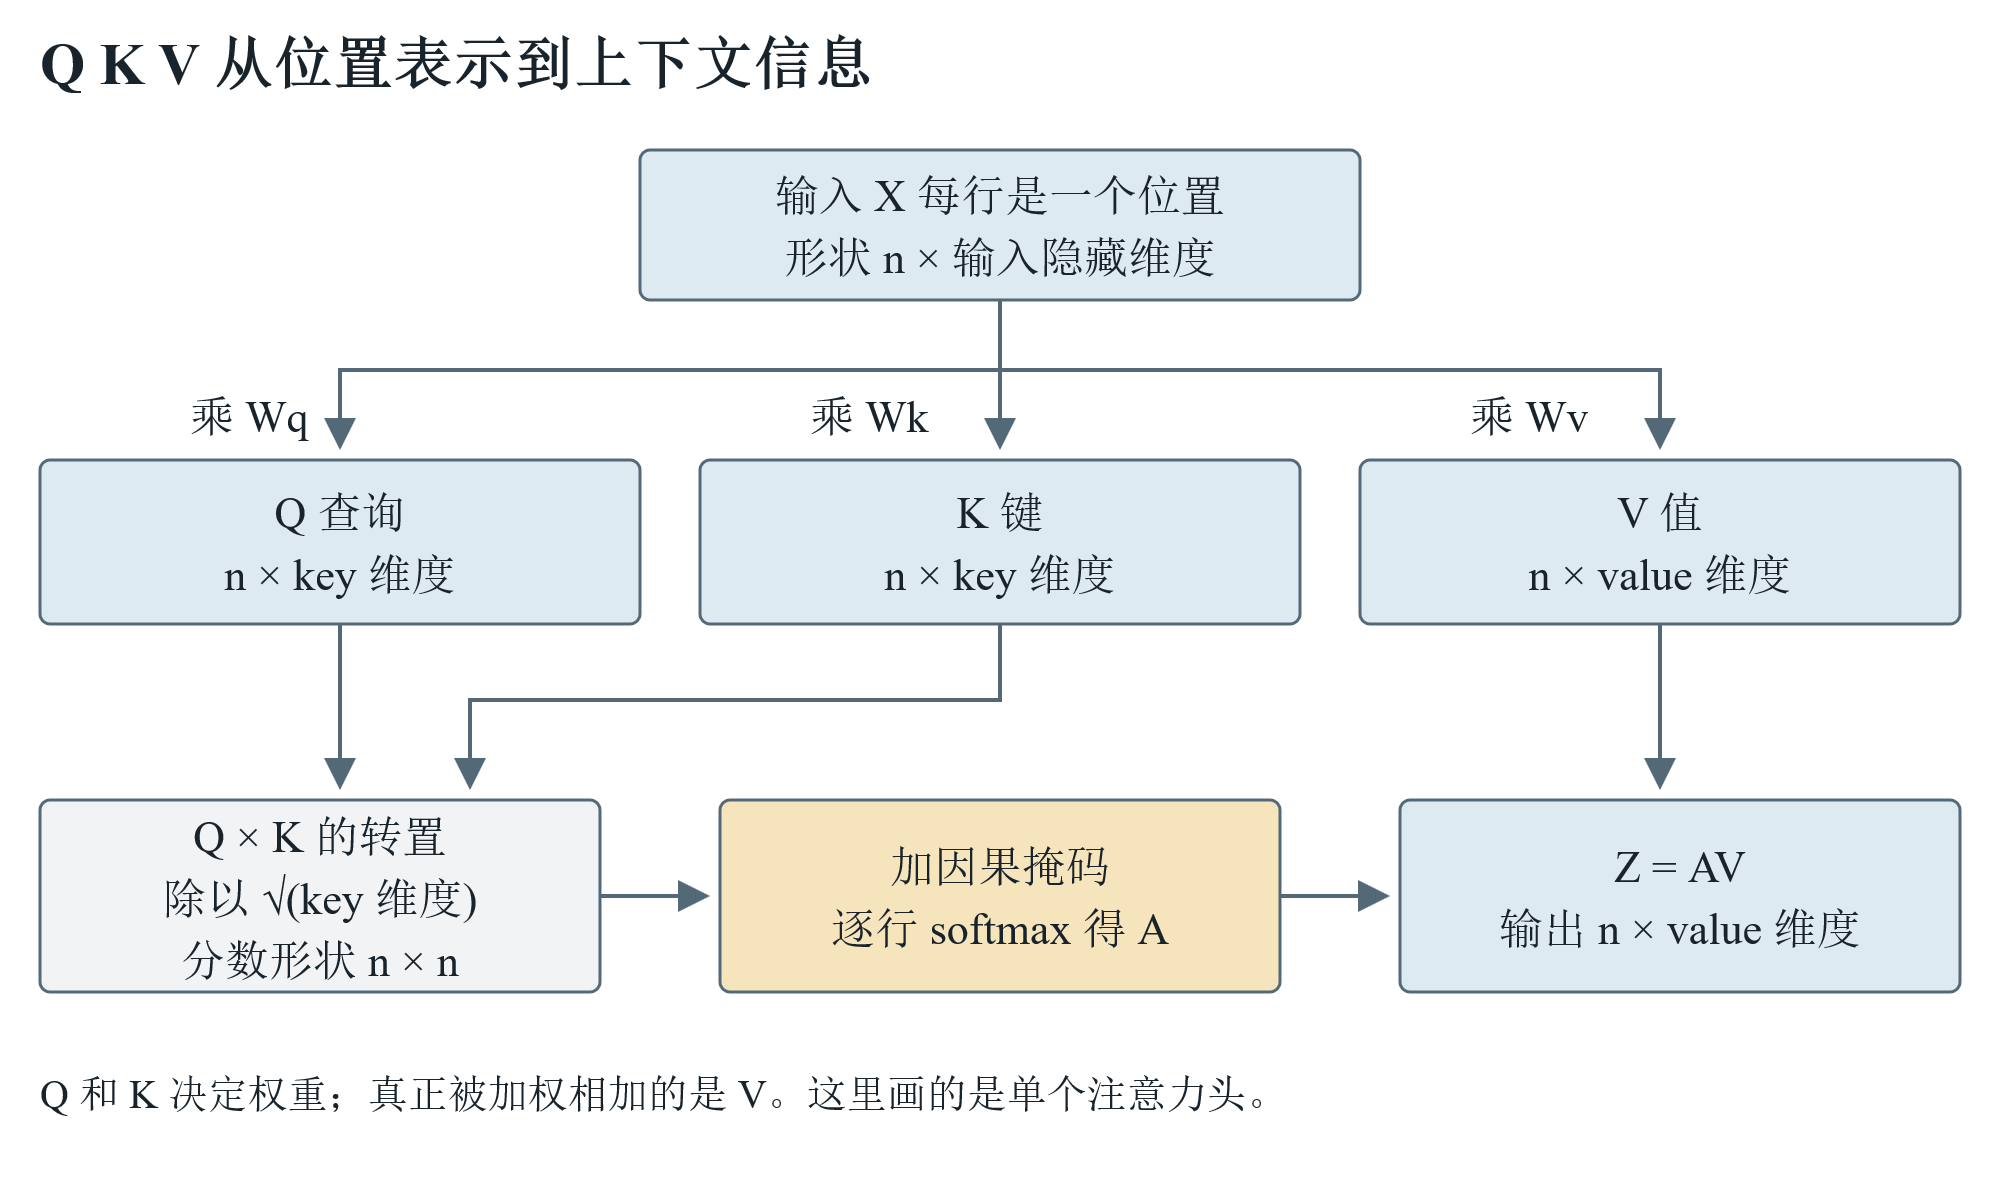
\includegraphics[width=\linewidth]{assets/media/image6.png}
    \caption{单头注意力的数据流。Q 与 K 产生位置之间的分数；掩码与 softmax 得到权重矩阵 A；再由 A 对 V 做加权和。n 是序列长度。}
    \label{fig:QKV计算}
\end{figure}

\textbf{沿着一行真正算一次} 我们暂把``小猫 追球''当作三个玩具 token，站在第二个位置``追''上。本例人为设定了该位置的 q\ensuremath{{}_{2}}，以及三个位置的 key 与 value；这些数只用于复算，并非从真实模型提取。q\ensuremath{{}_{2}} 与三个 key 的点积分别是 1、0、1，除以 √2 后为约 0.707、0、0.707。

第二个位置只能读取第一、第二个位置，第三个位置是未来，因此先把第三个分数置为负无穷，再对这一行做 softmax。前两项得到约 0.670 和 0.330，第三项为 0；最后用这三个权重加权 value，而不是把 key 当作输出。计算结果是约 (1.340, 0.660)。

一个 query 的完整计算：softmax 在允许的位置之间归一化；禁止位置的权重为 0，不能先读未来信息再在输出端补救。

注意，``追''位置更新后的表示可以用于预测后续 token，但当前这次注意力不能把未来``球''的内容拿来使用。训练时整段序列虽然并行送入模型，掩码仍保证每一行只有相应前缀可见。图 \ref{fig:QKV计算} 的 n × n 分数矩阵，就是同时对所有 query 做这样的行计算。

多头注意力把多套投影的结果拼接，再经过输出投影，回到能够与残差相加的隐藏维度。若采用 RoPE，位置相关旋转施加在 Q 与 K 上再计算分数，图 \ref{fig:QKV计算} 省略了这一环节以突出核心数据流；不能因此把位置编码理解成另一份 V。注意力权重也只是这次前向计算的系数，不自动等于因果解释，第九部分会专门检验这一点。

注意力后还有前馈网络、残差连接和归一化。残差让每一层在已有表示上修正，归一化帮助维持适合优化的数值尺度，前馈网络对每个位置做非线性变换。若使用混合专家（Mixture of Experts，MoE）架构，路由器只激活部分专家；这能改变计算与参数容量的配比，但还带来通信、负载均衡和部署问题，并非免费扩大模型。

我们把常见的先归一化（pre-norm）解码器层画在图 \ref{fig:一个Transformer层}。第一条支路通过注意力从其他允许位置取信息，再加回原状态；第二条支路通过前馈网络变换各位置，再加回。图中的归一化位置是这一具体结构的约定，不应推广为所有 Transformer 都完全相同。

\begin{figure}[t]
    \centering
    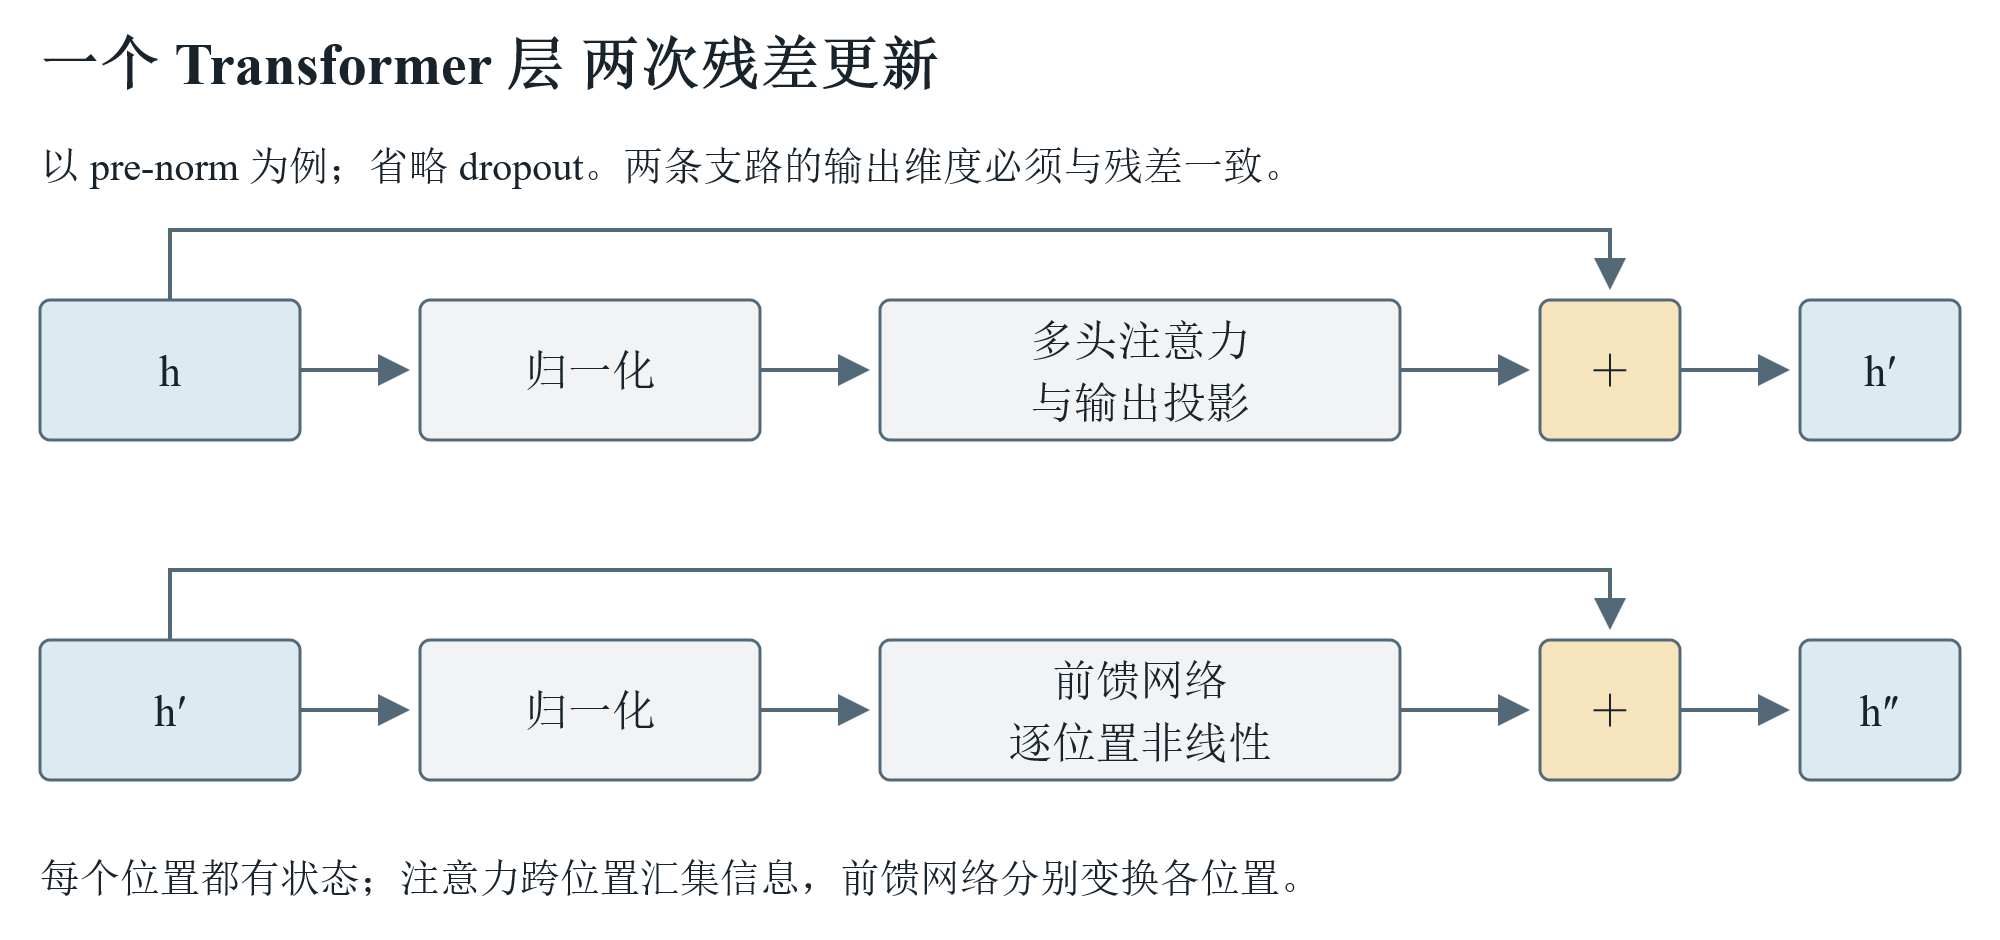
\includegraphics[width=\linewidth]{assets/media/image8.png}
    \caption{一个 pre-norm Transformer 层的两次残差更新。每次加号两侧形状必须一致；多层堆叠后才形成供输出头使用的上下文表示。}
    \label{fig:一个Transformer层}
\end{figure}

经过多层计算，当前位置的隐藏向量被语言模型输出头（Language Model Head，LM head）映射成词表大小的一组未归一化分数（logits）。logits 还不是概率；softmax 才把它们变成总和为 1 的分布。某些模型把输入 embedding 与输出权重绑定，某些不绑定。我们现在能把一轮生成完整地走通：token ID、输入向量、上下文表示、logits、概率，再到下一个 token。

\textbf{配合视频理解} 若 Q、K、V 的矩阵关系仍然抽象，我们可以在 B 站搜索``李宏毅 2021 自注意力机制 Self-attention''，选择包含完整计算过程的课程视频。边看边暂停，画出一次 query 与所有 key 比较、再加权 value 的过程。

\textbf{本节相关资料}
\begin{enumerate}
    \item Vaswani 等，2017，\href{https://arxiv.org/abs/1706.03762}{Attention Is All You Need} 。\textbf{点积注意力里程碑论文，但现在所有的注意力实现都已经不再用这种形式，而是改用 GQA 等高效注意力变体，可自行学习。}阅读重点：注意力计算、多头结构与残差。原论文是编码器解码器结构，阅读时区分它与纯解码器语言模型。
    \item Ba 等，2016，\href{https://arxiv.org/abs/1607.06450}{Layer Normalization} 。阅读重点：归一化解决哪一类优化困难。
    \item 苏剑林等，2021，\href{https://arxiv.org/abs/2104.09864}{RoFormer Enhanced Transformer with Rotary Position Embedding} 。阅读重点：RoPE 怎样通过旋转查询和键，把相对位置关系带进注意力分数。\textbf{中国最重要的大模型研究成果之一，\href{https://spaces.ac.cn/}{苏剑林博客}\footnote{https://spaces.ac.cn/}非常值得阅读。}
\end{enumerate}

\section{预训练与缩放定律 怎样分配训练资源}\label{预训练与缩放定律 怎样分配训练资源}

我们终于可以训练一个toy模型。第一轮输出近乎乱码，训练一段时间后出现词语，再后来句子逐渐连贯。这个过程容易让我们只盯着损失（loss）曲线。可要理解曲线，我们需要先看一次参数更新。

我们从语料抽一个小批次（batch）\footnote{训练时不会一条一条训，而是一次训多条样本，称为一个 batch，与传统机器学习概念一致。}，前向得到预测概率，计算交叉熵，再反向传播得到每个参数对损失的梯度。优化器按学习率调整参数。梯度表示当前位置的局部变化方向，不是对整段知识的显式存储指令。学习率太大可能让训练不稳定，太小可能在有限预算里进展缓慢；有一些缓解方案可以了解：自适应矩估计（Adaptive Moment Estimation，Adam）优化器的解耦权重衰减版本 AdamW（Adam with Decoupled Weight Decay）还会维护优化状态，因此训练显存不只是权重占用。过去很多年工程实践中最常用的是 AdamW，近期出现了一个非常有前景的方法叫 Muon（本节参考论文 3），正在被工业界大规模应用，可以自行了解。

预训练的数据管道同样属于训练方法。我们先清洗编码和模板噪声，去除大量重复，再考虑来源质量、语言比例与许可要求。重复数据会改变训练权重；污染评测集会制造虚假的泛化。把更多低质量文本送进训练，既不等于更多有效知识，也不保证更低的目标任务错误率。

当计算预算有限时，我们有三个可调节预算的选择：模型多大、训练多少 token、使用多少计算。\textbf{缩放定律（scaling laws）}描述在一定实验范围内，损失随这些量变化的经验规律。论文Chinchilla （本节参考文献 1）的重要启发是，\textbf{固定训练计算下，参数和数据需要共同增长}；只扩大模型却训练不足，会浪费潜力，比如对于一个80B模型的训练数据，用来给一个800B的模型训练，模型的最终表现就不会充分发挥。它给出的是在特定设置中拟合出的配比，不是适用于任意数据、架构和部署成本的永久常数。

我们可以把问题变成实验：用同一总计算预算，比较一个大模型少训练与一个小模型多训练。评价时既看验证损失，也看讲题任务。若大模型训练损失更低却验证更差，可能涉及过拟合、数据覆盖或比较预算不公平，不能仅凭参数量推断胜负。

部署会改变最优选择。如果助手要服务许多用户，稍小模型可能值得训练更久，以节省每次推理的成本；如果任务允许调用更强模型，路线又会不同。训练 scaling 与推理时增加采样或思考预算解决的是不同资源分配问题，我们在第七部分再把它们接起来。

\textbf{本节相关资料}
\begin{enumerate}
    \item Hoffmann 等，2022，\href{https://arxiv.org/abs/2203.15556}{Training Compute-Optimal Large Language Models}，也就是 Chinchilla 。阅读重点：固定计算预算如何分配给参数与数据。
    \item Loshchilov 与 Hutter，2017，\href{https://arxiv.org/abs/1711.05101}{Decoupled Weight Decay Regularization}。阅读重点：AdamW 中权重衰减与梯度更新的关系。
    \item Liu 等，2025，\href{https://arxiv.org/abs/2502.16982}{Muon is Scalable for LLM Training}。
\end{enumerate}

\section{幻觉与前缀错位 为什么会连贯地写错}\label{幻觉与前缀错位 为什么会连贯地写错}

预训练后，小助已经能流畅解题。我们问一个编造出来的课程规则：``本课允许迟交几天？''，实际上不允许迟交，但是它也给出一个听上去合理的数字。我们没有把规则交给它，它依然给出答案。这让我们意识到：预测token和确认一个事实对大模型来说是不同的事情。

参数里可以存储和组织大量知识\footnote{大模型训练属于一种信息压缩，把远超参数量的信息压缩到有限的参数中。}，但生成时没有一个自动运行的``事实查表保证''。语料可能过时、相互矛盾或压根不含这个问题的答案。上下文又常暗示``这里应该继续回答''。因此，模型可以生成结构完整但依据不足的内容。我们不能把幻觉说成每个 NTP 模型都必然出现的严格数学定理；更有用的结论是，NTP 本身没有提供逐条事实保证。

另一个风险来自前缀。训练时，我们通常把真实序列的此前 token 交给模型，监督训练下一位置是否出现正确的token。推理时，前缀则包含模型自己刚生成的内容，这就是自回归生成。

小助解题时若第一步误写成``21 除以 3 等于 6''，这一步已经错了，但是后续生成的内容依然看起来合理。训练数据里的标准解从未出现这个前缀，模型不一定学习过从这里纠正错误。训练前缀和实际生成前缀的错位，是暴露偏差（exposure bias）所指的一类问题。

我们把三种幻觉错误分开。1.上下文缺少规则，主要是知识或信息获取问题，即上下文不充分；2.知道题意却输出错误步骤，可能涉及模型学习过的计算与策略；3.第一步错后持续自洽生成，涉及推理错误轨迹的自我恢复与训练分布。对应的实验也不同：1.提供真实资料，观察能否纠正事实；2.提供正确中间步骤，观察能否完成剩余推导；3.故意放入错误前缀，观察能否发现并修正。这里的幻觉问题也是许多公司在面试时经常问的问题。

注意，大模型幻觉之前以及现在都是一个主流的研究方向之一，但随着模型本身智能的增强，幻觉问题很大程度上被缓解，这意味着一些热门问题可能是阶段性的，甚至在一定的历史条件下会被完全消除。

\textbf{本节相关资料}
\begin{enumerate}
    \item Zhang等, 2025, Detecting hallucination in large language models through deep internal representation analysis，\href{https://arxiv.org/abs/2405.19648v1}{https://arxiv.org/abs/2405.19648v1}。我们组张鸾在 2025 年发表的关于幻觉检测的论文。
\end{enumerate}


\chapter{嵌入表示与语义检索}\label{嵌入表示与语义检索}

除了 3.2 以外可略读，3.2 讲解如何训练 BERT 模型，这种模型专注语义嵌入，在许多场景中仍然重要。还要理解 BERT 模型和 Transformer 模型的差别是什么。

\section{从关键词匹配到语义向量 为什么文字不同也能找到答案}\label{从关键词匹配到语义向量 为什么文字不同也能找到答案}

第二部分结束时，小助已经可以把一段问题接着写下去。我们现在给它增加一个很朴素的任务：学生问``为什么不等式两边乘负数要变号''，请它先从课程资料里找出相关解释。资料明明写着``一个不等式的两边同乘负数，不等号的方向必须反转''，简单的逐文字匹配却可能把这段排得很靠后，两句话字面上差距很大。问题不在于小助不会说话，而在于它还缺少一种寻找材料的办法。

最直接的方法是数一数词语出现了多少次。把查询和文章切成词，比较共享的词，词频高、在整个资料库中又较少见的词通常更有区分力。词频－逆文档频率（Term Frequency--Inverse Document Frequency，TF-IDF）和最佳匹配 25（Best Matching 25，BM25）都是这条路线上的代表。它们并非只能比较两个原始字符串：文本先被切分和赋权，然后才计算匹配分数。但如果学生换了说法，材料恰好用了另一种表述，关键词的重合程度就不一定能准确代表相关程度。

我们想让``同乘负数要改变不等号方向''和``负数乘不等式为什么变号''容易匹配，同时又让``负数相乘的运算法则''和``不等式两边同乘正数''与它区分开。这里要求的不是``文字看上去像''，而是``这段资料能不能解决这个问题''。两个句子可能谈同一个话题，却只有其中一个真正回答了问题。

一种办法是把文本映射成固定长度的数值向量，称为嵌入表示（embedding）。我们用 f 表示这个映射：输入一句话或一段资料，输出一个 d 维向量。d 是模型约定的维度，例如几百或上千维，并不是一句话的字数。每个维度的数值没有天然固定的语义，向量之间的关系来自模型的训练。
\[e\  = \ f_{\theta}(\text{text}\mathbb{)\  \in \ Rᵈ}\]

式中 text 是输入文本，e 是最后得到的向量，θ 是产生向量的模型参数。注意，向量化不是稠密嵌入的独有本领。独热表示（one-hot）同样用数字表示文本：如果词表有一万个词，就可以把每个词表示成一万个位置中只有一个位置为 1 的向量。它能准确标记词的身份，却无法仅凭这种表示把``改变方向''和``反转不等号''判断为语义相近。稠密嵌入把可学习的信息压进较少的维度，期待相关文本在某种打分规则下更容易靠近。

所谓``靠近''需要一个具体指标。例如余弦相似度（cosine similarity）比较两个非零向量的方向，而不是直接比较字面词语。对两个句子向量 u、v，有：
\[cos(u,\ v)\  = \ \ \frac{(u\  \cdot \ v)}{\| u\| \ensuremath{{}_{2}}\ \| v\| \ensuremath{{}_{2}}}\ \]

点号表示各维相乘后求和，双竖线表示欧氏长度。若先把向量归一化到单位长度，余弦相似度就等于它们的点积。不过并非每一种模型都用余弦，也并非所有任务都需要归一化。真正重要的是：训练时怎样规定相关性，使用时就要按相应方式比较。

我们做一个没有训练的思想实验。给三段材料随意安排三个二维坐标，即使画出来很漂亮，也没有理由相信正确答案离问题最近。几何本身不会产生语义；\textbf{是训练信号让某些语义关系逐渐反映到几何关系里。} 因此，现在的问题不再是``怎么计算两个向量的距离''，而是``模型为什么会把应该匹配的文本放近''。

早期的 word2vec 通过词与上下文的共现规律学习词表示，说明仅靠语言数据就可能形成有用的几何结构。它通常为一个词学习较固定的表示；同一个英文 bank 出现在``存钱的银行''和``河岸''里，却有不同含义。上下文模型能够依据整句话改变某个位置的隐藏向量。我们在第二部分学过的 Transformer 已经具备这种上下文计算能力，但它的输入嵌入表、每个 token 的隐藏状态、表示整段文本的检索向量，仍然是三个不同对象，这告诉我们训练目标不同，嵌入表示的作用也就有差异。

\section{Bert模型 怎样把相关文本训练得更近}\label{Bert模型 怎样把相关文本训练得更近}

我们已经知道，训练不是给每个词写一个固定的``意思坐标''。那能否直接取出小助第二部分学到的 Transformer 层，把一句话送进去，再把隐藏向量平均一下，立刻得到好用的检索模型？我们试了试，发现有时同主题但不能回答问题的材料排在前面，真正有用的答案却排在后面。

这不奇怪。Transformer 这种自回归语言模型主要学习``在此前 token 给定的情况下，下一个 token 应该有怎样的概率''，这就是 Transformer 模型的目标，换句话说，Transformer 模型不是为了语义分类这个目标训练的，而Bert 模型就是为了这个目标训练的。会预测后续文字，不等于天然会给相似的句子之间做相关性排序。

要把已有模型变成用于检索的嵌入模型，我们至少需要两样东西：先定义\textbf{如何从一整段文字得到一个固定长度向量}，再定义\textbf{什么样的向量关系算训练成功}。

第一件事从架构开始。文本经过 tokenizer 变为 token ID，再经过 Transformer 产生每个位置的隐藏状态。我们可以取一个约定位置的状态，或对若干位置的状态求平均，把长度不一的句子变成同样维度的向量；这一步通常叫池化（pooling）。模型还可能再接投影层（projection），最后按训练约定进行归一化。对于使用 BERT 一类双向编码器的模型，可以利用双向上下文；对于以因果解码器为基础的模型，也可以通过特定位置、提示和训练方式得到句向量。没有一种池化方式适合所有架构。

\begin{figure}[t]
    \centering
    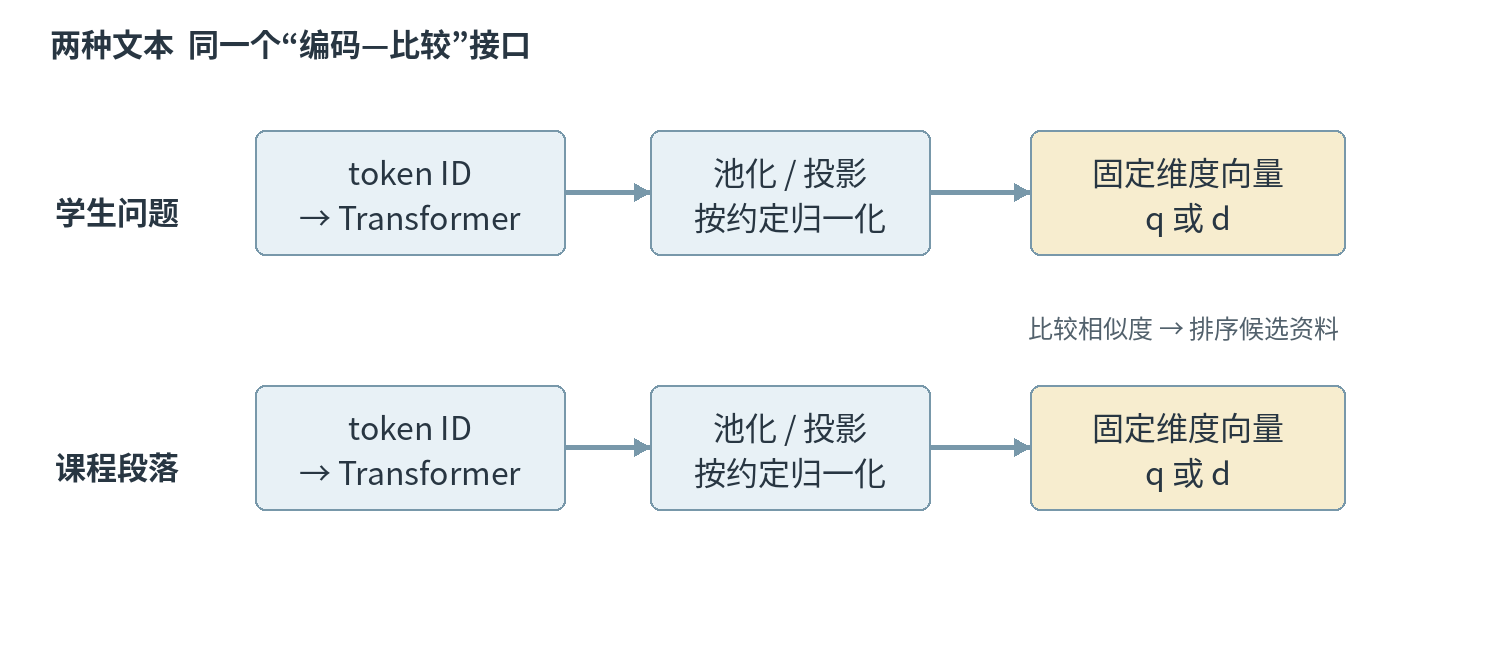
\includegraphics[width=\linewidth]{assets/media/image10.png}
    \caption{从整段文本到检索向量。输入 embedding 是 token ID 的查找结果；Transformer 的隐藏状态随上下文变化；池化以后才得到用于比较的整段文本向量。图示只是一种常见实现，具体模型还可能使用不同的提示、投影与归一化。}
    \label{fig:文本到向量检索}
\end{figure}

现在我们用同一个编码过程处理``问题''和``资料''：一个编码器得到查询向量 q，另一个编码器得到文档向量 d，再比较二者的相似度。这种分别编码的结构常称为双编码器（dual encoder），或形象地叫双塔结构。两边可以共享参数，也可以使用不同参数；有些模型还要求给查询加``query:''前缀、给文档加``passage:''前缀。这些不是装饰文字，而是训练时输入接口的一部分。

为什么要分成两边编码？如果课程库有十万条材料，可以先把十万条资料都编码一次并保存。学生每问一道题，只需要编码新问题，再与已经保存的资料向量比较，这就是 RAG 的常用方案。另一条路线是把``问题＋候选段落''一起送进模型评分，通常称为交叉编码器（cross-encoder）。后一种方式能够让问题和段落逐 token 交互，可能更精细，却难以对整个大型资料库逐条重算。双编码器牺牲了一些交互表达能力，换来了大规模预编码和快速检索。

第二件事才是训练目标。我们拿出一道查询 q：``为什么负数乘不等式两边需要变号？''准备一段正确资料 d\ensuremath{{}^{+}}：``两边同乘负数会颠倒大小关系，故需反转不等号。''再找两段不适合回答它的资料，例如``等式两边同乘一个数仍相等''和``负数乘法的符号规则''，记作 d\ensuremath{{}_{1}}、d\ensuremath{{}_{2}}。模型每次分别编码它们，给出分数。我们希望正确段落的分数高于其他候选，这样就可以训练模型，使得模型的嵌入能力实现此目标。

如果我们只告诉模型``这两个句子很像''，它可能学会把所有数学句子都放在一起。更有效的办法是让它在同一批候选里作出区别。这就是对比学习（contrastive learning）的直觉：不是预先规定每个向量的坐标，而是通过``谁应该更近、谁应该更远''的比较，反向更新编码器。

一种常见训练目标是信息噪声对比估计（Information Noise-Contrastive Estimation，InfoNCE）。为简化记号，假设一个查询对应 K 个候选文档，其中 d\ensuremath{{}^{+}} 是唯一被标注的正样本，s(q,d) 表示相似度，τ 是正的温度参数。单个查询的损失可以用 softmax 函数写成：
\[L\  = \  - log\ \{ exp\frac{s\left( q,d^{+} \right)}{\tau}/\sum_{\left\{ j = 1 \right\}}^{K}{\exp\frac{s(q,d_{j})}{\tau}}\ \ \}\]

分母把 K 个候选都算进去，包含正样本；分子只取正样本。这个比值可以看成：在当前候选集合里，模型给正确材料分配了多大的相对概率，前面加了个负号，所以通过梯度下降优化 L，就实现这个概率的提升。若四段资料分数都一样，模型只能给正确段约四分之一的概率；若正确段的分数明显高于其他段，损失就会下降。梯度从损失传回池化、投影和 Transformer 中实际参与训练的参数，使下一次编码后的几何关系有所改变。它不是把某条资料的坐标人工移动一下。

τ 控制分数差异在 softmax 中被放大的程度。较小的 τ 会使高分候选之间的差异更突出，但也可能放大错误标签或造成训练不稳定。实际训练还要决定 batch 大小、向量归一化、学习率，以及哪些参数更新。我们暂时不背配置，先看一条样本怎样提供有效信号。

\begin{figure}[t]
    \centering
    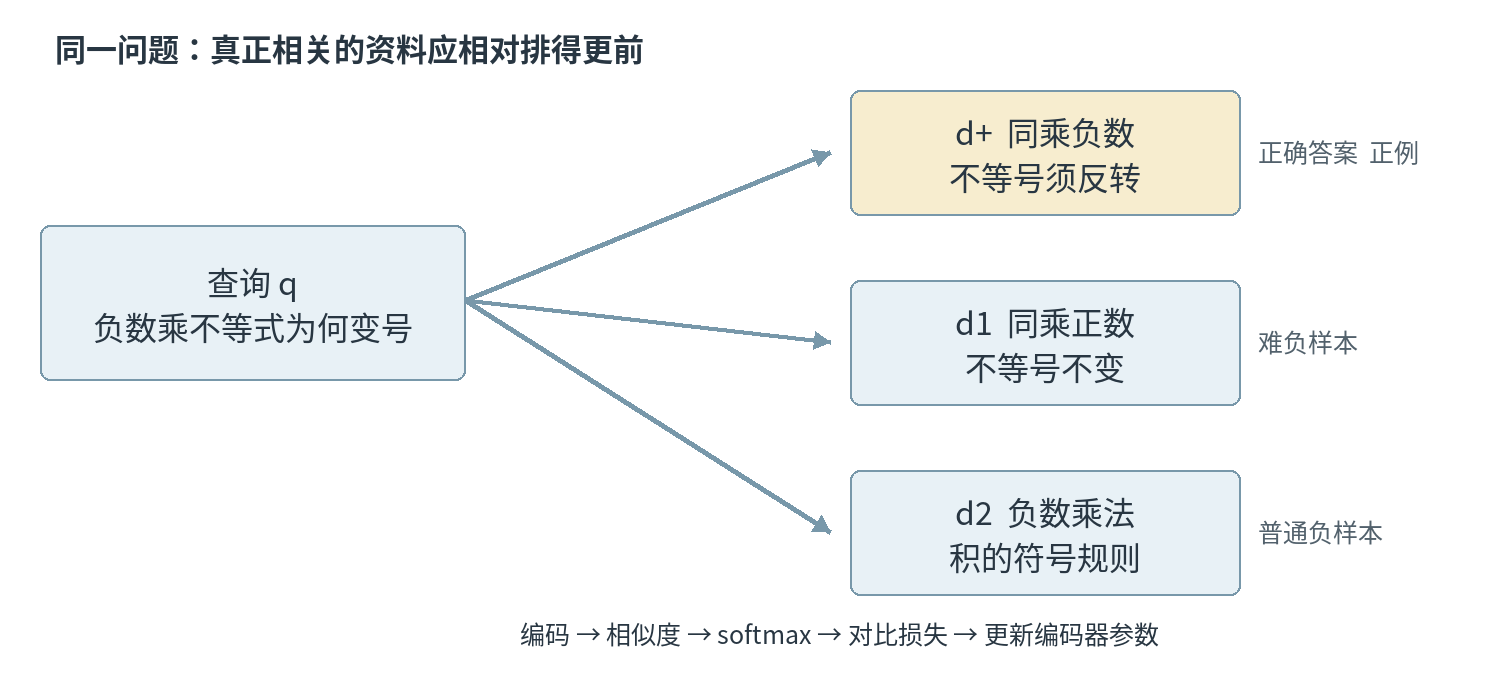
\includegraphics[width=\linewidth]{assets/media/image11.png}
    \caption{一次查询的对比学习。正样本要相对提高分数，负样本提供比较对象。与问题措辞接近却答错关键条件的难负样本，往往比完全无关的材料更能揭示模型是否学会了正确区分。}
    \label{fig:一次对比学习}
\end{figure}

一个 batch 中还可以放入多道查询及各自的正确资料。对查询甲而言，其他查询的资料可以当作负样本，这叫批内负样本（in-batch negatives），让一次前向计算产生许多比较。但它有一个风险：某段``别人的正确资料''其实也能回答查询甲。我们误把它标成负样本，训练便会错误地把两段有效答案推远。这种情况称为假负样本（false negative）。因此，更多负样本并不自动意味着更高质量。

我们再让小助检索``负数乘不等式为什么变号''。一种难负样本（hard negative）是``等式两边同乘负数仍保持相等''：出现了很多相同的词，也包含正确数学叙述，却没有解释不等式的方向变化。模型若能把这样的材料排在真正答案后面，才说明它学到了超出关键词重合的区别。难负样本可以从 BM25 或旧版嵌入模型的高分误召回中挑出，但必须核查它确实不满足问题，不能把另一种正确解法误判为负例。

训练数据从哪里来？可以人工编写问题与答案段落；可以从人工确认的问答资料中整理；也可以让强生成模型根据已有段落提出问题，再对生成结果进行核验。大量弱监督文本对可用于建立广泛的检索能力，之后再用目标课程里的高质量问题－资料对做适配。两阶段只是常见思路，不是所有嵌入模型必经的固定流程。点击日志也能提供信号，但点击往往受展示位置影响，不能直接当作无偏的相关性真值。

有了这些材料，我们才说清了``怎样训练 Embedding 模型''：选择预训练过的编码骨干，定义句向量的产生方式，组织查询、正例和负例，用对比目标计算损失并反向更新，再拿未见问题评价排序。如果直接从零训练也不是不可能，只是通常需要更大量数据与计算。一个检索模型是否好用，最终取决于它对目标查询的排序，而不是其向量图看起来多么整齐。

\textbf{本节相关资料}
\begin{enumerate}
    \item Reimers 与 Gurevych，2019，\href{https://arxiv.org/abs/1908.10084}{Sentence-BERT: Sentence Embeddings using Siamese BERT-Networks}。阅读重点：为什么需要专门面向句子相似度训练的模型，而不是把普通语言模型的表示直接当作检索结果。\textbf{这类做句子级嵌入的模型称为 SentenceTransformer，在现代自然语言任务中仍然常用，比如 \href{https://huggingface.co/Xenova/all-MiniLM-L6-v2}{all-MiniLM-L6-v2}。}
\end{enumerate}

\section{从语义向量到真正的检索 为什么不应直接淘汰关键词检索}\label{从语义向量到真正的检索 为什么不应直接淘汰关键词检索}

我们训练出了一个嵌入模型。小助输入问题，模型给出查询向量；资料库里的段落也都有向量。接下来似乎只需挑出余弦相似度最高的几段材料。但在开始宣布``语义检索替代了旧检索''之前，我们给它增加两道题，看看它会在哪里失败。

第一道题是``怎么解释负数乘不等式要变号''。课程材料可能写作``同乘负数须翻转不等号''。两句话表面措辞不同，意义与任务却对应。训练合适的稠密检索（dense retrieval）往往能弥补词面匹配的不足，特别是在改写、同义表达和跨句联系比较多的场景。这里的收益不是因为向量计算比字符串计算更神奇，而是编码器在大量文本对上学会了什么样的相关关系。

第二道题是``请找出课程文件中的习题 A-017''。如果资料库恰好含有``习题 A-017''和``习题 A-018''，它们在主题与句式上可能极为接近；向量却未必把编号的单字符差异视为最重要的区别。此时基于关键词的 BM25 或精确字段匹配可能更加可靠。课程版本号、日期、代码标识符、人名和罕见术语也常有类似问题。使用 Embedding 并不意味着可以放弃精确匹配。

我们因此不把检索方法排列成``越新越好''的清单，而是按错误类型选择。词法检索依赖文本中的明确词项，适合精确名称和稀有关键词；稠密检索根据学得的向量关系，适合字面不同但任务相关的表述。两者可以并行取候选，再把结果融合，这叫混合检索（hybrid retrieval）。常见的做法是合并排名或按校准后的分数加权；不同系统的原始分数通常不能不经处理就直接相加。

在资料只有几百段时，最简单的做法是把查询向量与每个资料向量都算一次相似度，得到精确的向量近邻排序。如果资料变成百万段，这样逐条比较就会消耗较多时间和计算。传统机器学习方法中，近似最近邻（Approximate Nearest Neighbor，ANN）索引通过组织向量、减少需要比较的候选，换取更高检索速度，但可能漏掉真正的高分段落。因而 ANN 解决的是``怎样更快找到已有向量的近邻''，不是``怎样训练出更有语义的向量''。

我们把整个过程按先后顺序写清楚。离线阶段，先整理资料，按适当段落切分，为每一段保存标题、来源、版本和标识，再用同一嵌入模型编码并建立索引；在线阶段，把学生问题按查询侧的约定编码，找出 top-k 候选，需要时合并关键词检索结果。若前面还有很多候选，也可以让问题和文档共同输入更精细的重排模型（reranker），再决定最后保留哪些资料。检索的输出是``值得阅读的候选''，并不是已经核实的最终答案。

这条链路会引出两类看起来相同、原因却不同的失败。假如一段正确材料在全量向量暴力搜索时就排在很后面，那么需要检查训练数据、查询写法、文本截断或编码模型；假如暴力搜索能找到它，但 ANN 查询遗漏了它，就优先检查索引设置和搜索预算。如果正确材料本来不在库中、版本已经过期，换一个更强的嵌入模型也找不回不存在的证据。

我们还需要防止``相似''被当作``正确''。学生问``作业最晚什么时候提交''，模型找出一段内容为``上学期作业截止时间''的文字，主题完全吻合，却不能回答当前日期。语义向量往往能指出讨论的是同一种事情，但未必可靠处理新旧版本、权限或细粒度条件。建立资料库时保存并使用版本、时间和来源，必要时做明确过滤，比盲目提高相似度阈值更有用。

现在给小助设计一次可以复核的检索实验。我们先标注二十个尚未参与训练的课程问题，以及每题真正能够回答它的段落。让 BM25、嵌入检索和混合检索使用同一份资料，分别记录前五名有没有出现正确证据。如果我们只为每题选定一段标准证据，可以报告 Hit@5（前五名命中率）：看有多少题在前五名里找到了指定的正确段落。若给每题标注全部相关段落，也可以报告 Recall@5（前五名召回率），这时应计算找回了多少条相关段落、共有多少条相关段落。不要混用指标口径。

如果 Embedding 在改写问法上优于 BM25，却在编号题上退步，这不是``实验失败''，而是找到了它的适用条件。我们再查看失败样本：正确文档是否存在，相关性标注是否准确，向量模型是否把同主题错误答案排得过高，ANN 是否漏召回，混合检索是否真的互补。三种方法要在相同候选库、相近延迟或明确的计算预算下比较，不能让其中一种悄悄多看资料。

同一个嵌入空间还可以辅助找近似重复资料、组织主题或筛选异常样本。但``两个段落很像''不足以说明其中一个该被删除，``二维降维图上分成三团''也不足以证明主题一定正确。每换一种使用方式，我们都要重新定义要保留什么信息、要接受什么错误。

走完这一轮，小助终于拥有了在资料库里找线索的能力。我们理解了它来自怎样的训练：预训练模型提供上下文表示的基础，池化等操作给整段文字一个可比较的向量，文本对与对比学习让``能回答问题''逐渐变成可排序的关系，检索系统再把这种关系用于实际资料。与此同时，找到材料不等于已经读懂材料，更不等于自然会按学生的要求讲解。对于已经找回的证据，小助还需要学会怎样作答。

\section{基于大语言模型的现代 Embedding}

我们已经让小助能够从课程资料中寻找证据，但还有一个问题没有展开：第二章训练的是善于预测下一个 token 的大语言模型，为什么到了语义检索，却好像必须换成 BERT？如果我们手里已经有一个训练充分的大模型，能不能利用它读过的大量文本，直接训练出更好的检索向量？现代 Embedding 的一条重要路线，正是把预训练的大语言模型改造成文本编码器。本节沿着一次改造，看看向量从哪里来、相关性怎样学会，以及这种做法能解决什么问题。

先把架构与训练目标分开。BERT 和我们在第二章讨论的纯解码器（decoder-only）语言模型都建立在 Transformer 上。BERT 通常使用双向注意力，并以掩码语言建模等目标预训练；因果语言模型则遮住未来位置，主要学习下一个 token 的条件分布。BERT 的预训练也不是直接学习``哪些句子应该更相似''。两类骨干都可以经过专门训练得到句向量。因此，现代 Embedding 的变化，是利用另一种预训练起点，再重新规定输入、读出方式和优化目标。

从预测下一个 token 到读出整段文本

我们先把问题``为什么不等式两边乘负数要变号''送入一个因果语言模型。tokenizer 得到长度为 \(T\) 的序列，输入嵌入表把各个 ID 变成向量，多层 Transformer 再输出 \(T\)个上下文隐藏状态。设最后一层输出为：
\[H = \left( h_{1},h_{2},\ldots,h_{T} \right),\quad\quad h_{t} \in \mathbb{R}^{m}.\]

这里的输入向量是查表结果，\(h_{t}\)是结合上下文计算出来的状态；我们最终用于检索的整段文本向量，还需要从这些状态中读出。

生成时，我们把隐藏状态交给语言模型输出头，得到词表上的 logits，再预测后续 token。做 Embedding 时，常见做法是在输出头之前取隐藏状态，经过池化，必要时接投影，再按模型约定归一化。模型输出的是数值向量，通常不需要像聊天一样逐 token 生成一段回答。

因果掩码使第一个位置只能读到开头，后面的状态可以读到更长前缀，最后一个有效位置则能够关注整段已输入文本。这给出一个自然的读出办法：取最后一个有效 token 的最终隐藏状态，称为末词元池化（last-token pooling）。若最后一个有效位置为 \(t_{last}\)，则：
\[z = h_{t_{last}}.\]

如果训练约定在正文后追加序列结束标记（End of Sequence，EOS），我们就取 EOS 所在位置的状态，这通常叫 EOS pooling：
\[z = h_{EOS}.\]

EOS pooling 是一种特定的末位置读出，二者不能在所有实现中直接画等号。{[}3{]}{[}4{]}

这里的关键是``这个位置能读取全文''，而不是``最后一个词本身概括了全文''。假设所有问题末尾都加同一个 EOS，查表得到的 EOS 输入向量确实相同；但经过多层注意力后，它在不同问题中的隐藏状态可以不同，因为它汇集了不同的前文信息。后续的检索训练还会进一步推动模型，把任务需要的信息组织到这个读出位置上。

我们也不能反过来说，只要能看见全文，就已经把全文无损保存下来。一个固定长度向量需要压缩信息，训练会决定哪些差异值得保留。最后位置在因果结构上具备汇集全文信息的条件，并不保证未经适配的模型已经学会把``能回答问题''表现为余弦相似度。直接提取普通聊天模型的末位置状态可以作为基线，却不能据此认定已经得到高质量检索模型。

实际编码还有一个容易忽略的细节。不同长度的文本放进同一个 batch，通常要用填充 token（padding token）补齐。如果我们机械地取数组最后一列，就可能取到填充位置。应当依据 attention mask 和填充方向，找到最后一个有效位置；若模型要求 EOS，还要确保截断后保留了约定的结束标记。结束符、模板、截断和池化必须一起遵守模型接口，不能只看``输出维度相同''就认为实现等价。{[}4{]}

末位置读出也不是唯一选择。平均池化（mean pooling）可以汇总多个位置。设参与池化的有效位置集合为 \(\mathcal{V}\)，则：
\[z = \frac{1}{\left| \mathcal{V} \right|}\sum_{t\mathcal{\in V}}^{}h_{t}.\]

这里的有效位置通常不包含 padding，是否包含指令和特殊标记则由模型的训练约定决定。某些因果模型也会使用位置加权平均，让看到更长前缀的位置得到更大权重。另一条路线则改变注意力掩码，使每个位置都能读取左右上下文，再进行平均池化。哪一种更合适，要看模型怎样训练，不能推导出``LLM 一律用 EOS''或``改成双向就一定更强''。

把大模型放进双塔以后怎样训练

现在我们把问题和资料分别送入这个编码过程。查询侧得到 \(e_{q}\)，资料侧得到\(e_{d}\)，再通过点积或余弦比较。这仍然是前文的双编码器，也常叫双塔结构。``双塔''描述的是两段文本分别编码，不要求存在两份参数不同的大模型。查询和资料可以共享同一套权重，只使用不同的输入模板；由于查询侧含有任务指令，即使共享参数，两侧的实际输入与功能也可以不同。

我们可以用一组简写串起整条计算链：
\[{H_{q} = {LLM}_{\theta}\left( {template}_{q}(I,q) \right),
}{H_{d} = {LLM}_{\theta}\left( {template}_{d}(d) \right),}\]
\[z_{q} = {pool}\left( H_{q} \right),z_{d} = {pool}\left( H_{d} \right),\]
\[e_{q} = \frac{z_{q}}{\left\| z_{q} \right\|_{2}},\quad e_{d} = \frac{z_{d}}{\left\| z_{d} \right\|_{2}},\]
\[s(q,d) = e_{q}^{\top}e_{d}.\]

\(I\) 表示任务指令，\(q\) 是查询，\(d\)是资料，\(\theta\)是共享的骨干参数。template 表示输入格式约定，pool 表示池化。这里选用归一化后的点积作为示例，暂时省略可选投影层；并非每个 Embedding 模型都采用完全相同的接口。真正需要记住的是，查询和资料独立得到向量，评分时才把二者联系起来。

假如小助要查``为什么不等式乘负数要变号''，我们准备正确段落\(d^{+}\)，再准备一个措辞很像却只讨论``等式两边同乘负数''的 \(d^{-}\)。原来的语言建模目标主要要求模型提高真实下一个 token 的概率；现在的目标则要求查询向量与正确段落的相似度，相对高于错误段落。这是从生成训练转向表示训练的关键一步，换掉池化操作本身并不能完成这种转变。

仍以前文的 InfoNCE 为例，设候选集合\(\mathcal{C}\)包含正例和若干负例，单个查询的损失可写为：
\[\mathcal{L} = - \log\frac{\exp\left( s\left( q,d^{+} \right)/\tau \right)}{\sum_{d_{j} \in \mathcal{C}}^{}{\exp\left( s\left( q,d_{j} \right)/\tau \right)}}.\]

\(\tau\) 是温度参数，分母包含正例。如果正确段落和错误段落得分相同，模型就没有学会区分它们；降低损失会推动正确段落获得更高的相对分数。

梯度经过相似度、归一化和池化，回到参与训练的 Transformer 参数。我们可以全量更新骨干，也可以使用低秩适配（Low-Rank Adaptation，LoRA）等方法，只更新一部分附加参数。具体哪些参数改变由训练配置决定，并不是只训练输入嵌入表。

向量坐标因此随着编码函数一起变化。某次参数更新后，许多文本重新编码的结果都会改变，而不是只移动这次训练样本的坐标。部署时，资料库可以离线预编码，在线只编码新问题；但换了模型检查点、池化或资料模板，就应重新生成兼容的资料向量和索引。两个模型即使输出同样维度，也不意味着它们共享同一个坐标空间。

数据决定``相关''究竟是什么意思。同一句``负数运算''既可以按主题分类，也可以用于寻找解题证据。我们给查询增加``查找能够解释该数学问题的课程段落''这样的任务指令，就是要告诉模型当前应保留哪一种关系。指令感知的 Embedding 通过带任务说明的文本对训练，让指令能够影响最终向量。{[}3{]}

这类训练样本可以组织为：
\[\left( I,q,d^{+},d_{1}^{-},\ldots,d_{K}^{-} \right).\]

正例不必是查询的同义改写，也可以是一段真正回答问题的资料。负例可以来自批内其他文本，或者来自旧检索器召回的高分错误材料。我们仍要检查假负例：如果另一个段落也能解释变号，却被当成负例，模型就会收到相互冲突的信号。困难与正确是两件事，不能只按分数高低自动决定标签。

生成式大模型还可以参与构造这些样本。我们让它根据真实课程段落提出不同问法，覆盖初学者、不同语言和不同难度，再筛除答非所问、遗漏条件或与原文矛盾的配对。这时大模型可能承担两种角色：一个作为待训练的编码骨干，另一个作为数据生成器或筛选器。两种角色可以分开，不需要让在线检索器同时运行一套生成流程。合成数据扩大了训练覆盖，但教师模型的错误和表达偏好也可能被带入，因此仍要用独立的真实查询检查泛化。

\textbf{三条现代路线怎样作出不同选择}

LLM2Vec 回答的是``怎样把已有因果语言模型改造成双向文本编码器''。它先开放双向注意力，再用掩码下一词元预测（Masked Next Token Prediction，MNTP）适配新的信息可见方式，之后通过无监督对比学习改善序列表示，并使用平均池化。MNTP 保留了下一位置预测的移位形式，却针对被遮蔽的 token 计算训练信号；它不是简单把普通 BERT 的损失原样搬过来。需要时还可以进一步做有监督对比训练。

我们可以把这条路线理解为：保留预训练权重积累的语言基础，调整信息流动方式，再让模型适应新的表示任务。它说明 decoder-only 是一种预训练起点，不是改造后永远不能改变的限制。不过，只在推理时随手删除因果掩码，并不能等价复现 LLM2Vec 的训练过程；新的注意力模式需要与相应训练一起理解。

GritLM 关注另一件事：能否让同一套模型权重兼顾生成与 Embedding？它通过生成表示指令调优（Generative Representational Instruction Tuning，GRIT），把表示任务的对比损失与生成任务的语言建模损失结合起来。我们可以把联合目标简写为：
\[\mathcal{L}_{joint} = \lambda_{rep}\mathcal{L}_{rep} + \lambda_{gen}\mathcal{L}_{gen}.\]

其中，\(\mathcal{L}_{rep}\) 是表示学习损失，\(\mathcal{L}_{gen}\) 是生成任务的语言建模损失，两个 \(\lambda\) 控制各自权重。这只是帮助理解的简写，实际训练还涉及两类数据的采样比例、批次组织与损失归一化。

做 Embedding 时，GritLM 采用双向注意力和平均池化；生成时保留因果注意力。池化只汇总正文对应的最终隐藏状态，指令和格式 token 不直接参与平均，但仍能通过注意力影响正文状态。{[}2{]}

因此，``统一模型''不意味着同一次前向计算同时产生最佳向量和完整回答。两类任务仍有不同的输入、掩码与损失约定。GritLM 展示了共同训练的可行性，却不能证明任何聊天模型加一个池化层，就能自动兼顾两种能力。应用中是否值得共享模型，还要考虑服务调度、显存、延迟，以及我们是否真的同时需要两种功能。

Qwen3-Embedding 则展示了保留因果注意力的路线。其技术报告使用输入末尾 EOS 位置的最终隐藏状态作为文本表示，并通过多阶段对比训练适配相关性任务。查询侧包含任务指令，检索文档侧通常不加同样指令。它利用大规模合成文本对做弱监督训练，再结合高质量数据微调，并通过检查点合并改善泛化；不同阶段的对比数据质量和覆盖不同，不能把第一阶段简单理解为重新训练一次普通聊天模型。{[}3{]}{[}4{]}

这条路线让我们看到，双向化不是 LLM Embedding 的必经步骤。Qwen3-Embedding 把任务需要的信息训练到因果模型的末位置读出上；LLM2Vec 则改变可见范围后汇总各位置；GritLM 进一步兼顾生成目标。三者共同利用大语言模型的预训练基础，但对注意力、池化和任务组合做出了不同选择。复现时必须采用各自的完整配方，不能把一个模型的权重与另一个模型的模板或池化随意拼接。

\textbf{什么时候值得替换原来的编码器}

现在我们可以回答开头的问题。大语言模型经过充分预训练，已经形成丰富的上下文表示，也可能具备较好的多语言和复杂语句处理能力；表示训练有机会把这些基础转化为更好的相关性排序。遇到跨语言问法、复杂条件或代码检索时，这种起点可能带来收益。但收益来自骨干、数据、任务指令与优化的共同作用，不能只归因于``参数更多''，也不能从生成能力直接推导检索成绩。

代价同样具体。较大的骨干通常需要更多显存和编码时间，资料更新时还要支付重新编码成本。长上下文支持意味着模型能够接收更长输入，却不保证一个固定长度向量能保留长文所有细节；把整本教材压成一个向量，往往不如恰当切分后分别检索。嵌入维度还影响向量库容量和相似度计算成本，不能只比较模型参数量。

小型双向编码器因此仍有价值。若课程资料范围稳定、问法简单、延迟预算紧，小模型可能已经达到所需召回率。课程编号、公式符号和版本条件仍可能需要关键词或字段过滤；候选之间细微的条件差异，也可能需要交叉编码重排。LLM Embedding 扩展了可用的编码器路线，并不自动取代词法检索、小模型或重排系统。

我们可以给小助安排一个小实验：固定同一份课程资料和段落切分，比较普通因果语言模型的直接读出、已经训练好的小型嵌入模型，以及专门训练的 LLM Embedding。每个模型遵守自己的官方模板和池化要求；测试问题按改写、复杂条件、编号和跨语言分别记录。除前五名命中率外，还记录查询延迟、资料编码耗时和存储开销。若要判断``提升是否来自对比训练''，则需要在同一骨干和相同读出设置下比较训练前后，而不能仅比较两个名字不同的模型。

我们还应抽查那些主题相似却证据错误的结果。相关性分数不是事实正确率，也不是统一校准的置信度，不同模型的相似度阈值通常不能直接互换。如果大模型只在通用榜单上占优，在真实课程问题上却没有改善，我们就没有充分理由承担替换成本。相反，如果它能在可接受预算内稳定找回原先遗漏的证据，那么这才是更换编码器的实际依据。

走到这里，第二章和第三章之间的连接就清楚了：语言模型预训练提供可迁移的上下文计算能力，池化规定从哪里读出整段文本，指令与对比数据规定保留怎样的相关性，再由检索系统把向量用于寻找证据。小助可以继续使用独立的生成模型来阅读这些证据，也可以在经过专门训练的统一模型中切换任务。找到证据以后，怎样依据证据给出合适的回答，将继续把我们带向后面的训练与应用。

\textbf{实践}~检索增强生成现在（RAG）已经成为一种基本技能，尝试完整总结RAG的实现流程。

\textbf{本节相关资料}
\begin{enumerate}
    \item BehnamGhader 等，2024，\href{https://arxiv.org/abs/2404.05961}{LLM2Vec: Large Language Models Are Secretly Powerful Text Encoders}。阅读重点：双向注意力、MNTP 与对比学习分别解决什么问题。配合阅读\href{https://mcgill-nlp.github.io/llm2vec/tutorial/}{官方教程}。
    \item Muennighoff 等，2024，\href{https://arxiv.org/abs/2402.09906}{Generative Representational Instruction Tuning}。阅读重点：生成与表示怎样共用权重，以及两类任务的掩码、池化与损失怎样区分。可以参考\href{https://github.com/ContextualAI/gritlm}{官方实现}。
    \item Li 等，2025，\href{https://arxiv.org/abs/2506.05176}{Qwen3 Embedding: Advancing Text Embedding and Reranking Through Foundation Models}。阅读重点：因果注意力下的 EOS 读出、指令输入与多阶段对比训练。
    \item Qwen 团队，\href{https://huggingface.co/Qwen/Qwen3-Embedding-0.6B}{Qwen3-Embedding-0.6B 官方模型卡}。
\end{enumerate}


\chapter{监督微调与续训退化}\label{监督微调与续训退化}

\section{监督微调 SFT 用示范塑造助手行为}\label{监督微调 SFT 用示范塑造助手行为}

回到最初的方程题，我们给出一条完整示范：``先把两边除以 3，得到 a＋2＝7；再把两边减去 2，得到 a＝5；代回检验成立。''我们不只希望模型背下来这个答案，而是希望它在新题上也遵循解释、求解、检查的任务结构。

SFT 让模型在指令与对话上下文的时候，提高示范回答的概率。从训练目标看，它仍然通常是逐 token 最大似然；从数据看，它把我们关心的解题方法、思路、技巧等集中呈现给模型。示范可以由人写，也可以来自强模型或数据合成管线。

我们用掩码（mask）标出哪些位置计算损失，一般用户的问题是不计入训练的，模型只需要根据用户的输入做回答，我们希望训练的是回答的部分。常见做法是把不需要监督训练的 token mask 为 0，只对模型的回答部分进行监督训练，把系统提示词和用户提示词作为条件；多轮训练也可以监督多轮对话，因为用户通常是多次对话而不是对话一次就关掉会话但是需要注意的是，比如已经进行了几轮对话，现在对于用户新的问题，前面所有内容都是上下文，模型要参考前面的所有内容给出回答。简单来说，多轮对话可以拆成多条训练数据。把位置 t 的监督掩码记为 m 的下标 t，只对参与监督的 token 取平均，SFT 损失写为：
\[L_{SFT} = - \frac{1}{\sum_{t}^{}m_{t}}\sum_{t}^{}m_{t}\log p_{\theta}\left( x_{t} \mid x_{< t} \right)\]

求和号按序列位置相加，分母是有效监督位置数；若分母为 0，应拒绝该样本并检查数据处理，不能继续计算这个平均损失。m 为 1 的位置参与监督，为 0 的位置不参与，因为被 mask 掉的 token 的log p 乘以 0 就直接是 0。

图 \ref{fig:SFT监督位置} 把两个经常混淆的 mask分开。损失掩码决定哪些目标 token 直接计分，因果掩码决定预测这些目标时能读取哪些输入位置。常见实现会将输入与目标错开一位；若移位做错，模型可能在输入中直接看到被考查的答案。

\begin{figure}[t]
    \centering
    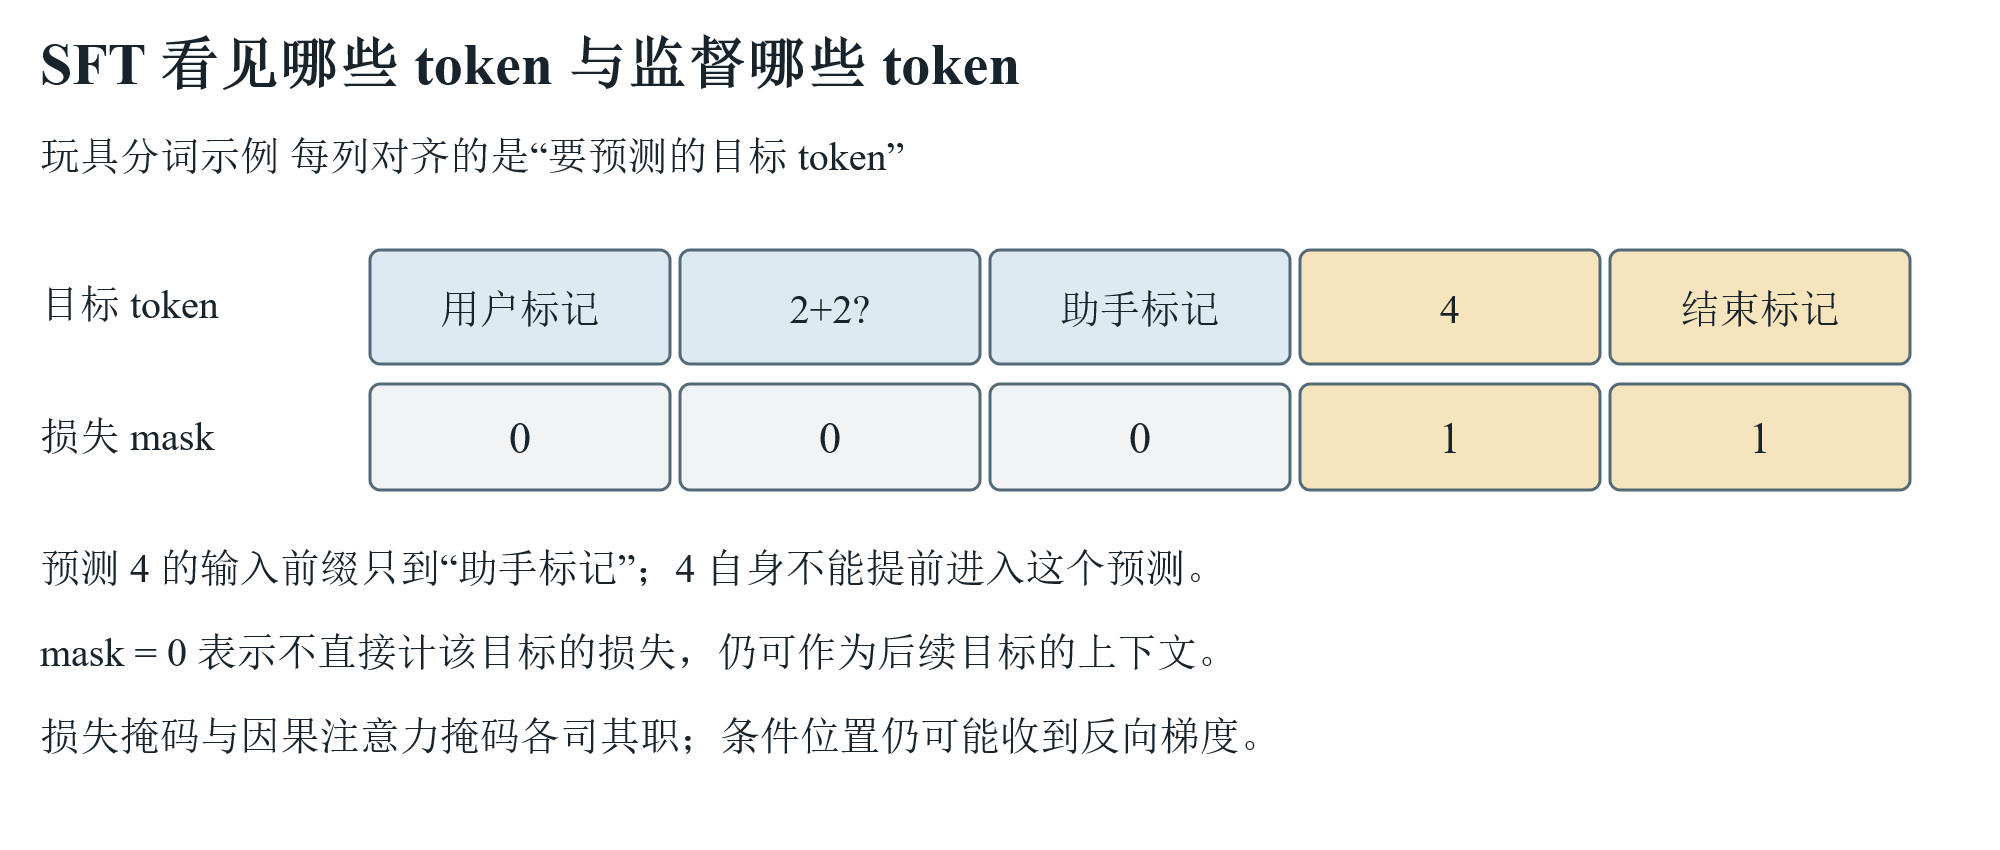
\includegraphics[width=\linewidth]{assets/media/image12.png}
    \caption{一条 SFT 样本的目标与损失位置。用户 token 即使不直接计损失，仍能作为助手回答的条件，其相关参数也可能经后续回答损失收到梯度。真实分词和模板可能拆成更多 token。}
    \label{fig:SFT监督位置}
\end{figure}

从行为克隆（behavior cloning）的视角，SFT 告诉模型``遇到这里，示范者这样走''。示范由外部给定，在本书的宽泛用法中属于异策略（off-policy）数据；它与学生当前生成的路径可能不同。它没有显式要求模型在多个候选中评判哪个更好。可我们也不能说它绝对学不到判断：若数据里包含批改、比较和自我纠错示范，模型同样可以学习这些行为。真正的区别是，普通最大似然并未直接优化独立的偏好比较或环境回报。

训练后，小助开始稳定给出分步答案。我们很高兴，却先在验证集核对：是否只学会了固定套话？是否每题都添加无意义检查？是否在资料不足时照样编造？格式是容易观察的进步，任务能力与可靠性还需要分别检查。

\textbf{实践}~注意，从这里开始就进入模型训练部分，推荐读者能够对每一个训练方法有一定的自主实践，后续大多数章节中不再单独给出实践建议。

\textbf{本节相关资料}
\begin{enumerate}
    \item Ouyang 等，2022，\href{https://arxiv.org/abs/2203.02155}{Training language models to follow instructions with human feedback}。即 InstructGPQ，前面多次参考到。阅读重点：监督示范在整个反馈训练管线中承担什么作用。
    \item Wei 等，2021，\href{https://arxiv.org/abs/2109.01652}{Finetuned Language Models Are Zero-Shot Learners}，FLAN 。阅读重点：任务多样性如何帮助指令泛化。
\end{enumerate}

\section{SFT 数据工程 模板与监督位置}\label{SFT 数据工程 模板与监督位置}

我们准备扩充 SFT 数据。最容易的做法是搜集尽可能多的问答，却发现质量逐渐失控：有的答案只给数字，有的先闲聊，有的把推理写错，有的缺少轮次结束标记。

我们先规定示范质量。方程题要求步骤正确、足够解释且不编造定理；资料题要求引用可找到、依据能支撑回答；信息不足题要求说明缺少什么。我们可以保留不同的表达方式，避免把多样性误当成噪声，但不保留彼此矛盾的任务要求，比如同一个问题我们给两种截然不同回答风格：一个花非常大的努力做深度推理，采样到一个非常长而详细的回答，另一个尽可能节约推理成本，尽量少验证，快速给出答案。模型对于同一个题目学习这两种完全不同风格的回答，就会导致行为冲突，具体可能表现为 grad norm 或者 loss 出现尖峰（spike），并且在训练完以后在推理时出现严重的复读现象。这体现出数据清洗的重要性。

训练前，我们随机抽取已 token 化的样本，检查角色边界、监督位置、最大长度与结束标记。若长样本总在最终答案之前被截断，小助就可能学会漫长推演，却学不到收束推导。

我们也会看分项损失。固定模板词频很高，模型很快学会``下面分步骤说明''这种习惯，总 loss 因此下降，但真正关键的算术 token 改善有限。这不表示格式一定``劫持''了学习，而是平均指标掩盖了不同位置的难度与价值。为了追求严谨，应该把格式正确率、答案正确率、步骤有效率都作为监控指标，防止只优化其中最容易的一项。

计算资源有限时，我们可以使用低秩适配（Low-Rank Adaptation，LoRA）。它冻结大部分基础权重，用低秩增量表达参数更新，减少可训练参数和优化状态。这个方法的思路非常简单但是非常重要，推荐读者自学，主要关注两点：一是如何节约计算开销，二是为什么 LoRA 单训一批小数据不太造成灾难性遗忘\footnote{灾难性遗忘是指这种现象：一个经过后训练的大模型在各方面能力达到均衡，此时用一个专项领域数据继续 SFT，导致其他各方面能力明显下降。这是许多任务里面需要考虑的问题。}。LoRA 解决的是适配成本与参数化方式，主要是大幅节约计算资源，无法修复坏数据，也不保证没有灾难性遗忘。秩（rank）、作用模块、学习率和数据量仍需要验证。全参数微调也并非总优于 LoRA，两者优劣应在清楚的预算和任务下进行\footnote{LoRA 系列方法在学术界受欢迎，因为计算开销大幅下降，可以做很多训练，但是在工业界大多不被支持，一方面是因为工业界有充足的数据资源和计算资源，二是因为对于各家自研模型来说，训练框架越简单越好，功能越少越好，否则难以维护，在这种情况下，LoRA 训练通常不被支持。}。

第一次小规模训练，我们故意让模型在少量干净样本上过拟合。若连这一步都做不到，先查管线；若可以学会，再扩大数据，观察泛化能力。任何系统性工程任务都需要预实验，对模型的上限和下限都有所了解。

\textbf{本节相关资料}
\begin{enumerate}
    \item Zhou 等，2023，\href{https://arxiv.org/abs/2305.11206}{LIMA Less Is More for Alignment}。比较有名的论文。阅读重点：高质量少量示范数据的训练价值可能非常大；但是也不要认为``少量数据总是足够''。
    \item Hu 等，2021，\href{https://arxiv.org/abs/2106.09685}{LoRA Low-Rank Adaptation of Large Language Models}。\textbf{（务必理解LoRA原理）}阅读重点：低秩更新节省了哪些资源，又没有保证哪些能力。即便不看论文原文也建议找资料理解 LoRA 如何高效训练。
\end{enumerate}

\section{续训退化 新任务变好为何旧能力变差}\label{续训退化 新任务变好为何旧能力变差}

小助已经会耐心讲题，我们想加入一门新课程，于是准备一批领域问答继续 SFT。为了节省标注，答案几乎都是一句话：``答案是 5。''\,``定义见第三章。''\,``选择 B。''新课程题的分数上升了，但小助对旧题也开始只给结论，不愿解释。

小助可能仍然有能力解释这些问题，只是在新训练分布下更偏向简短回答；也可能失去了某些步骤能力，这就是``灾难性遗忘''；也可能是对话模板变了（很少出现这种失误）。

更新为什么会波及旧任务？不同任务共享大量参数。新数据的梯度鼓励短答案，可能降低长解释的概率；新领域的词汇、格式、难度与采样比例，也会重新分配训练权重。

训练强度同样关键，通常学习率是 8e-5。相同的新数据，较高学习率、更多轮次的训练，都可能造成更大的参数漂移。反过来，过低学习率（比如 2e-5）也可能学不到新增任务。我们不能只说``把学习率调小''，而要在新任务收益和旧任务保留之间做曲线比较，用实验结果来验证猜想，合适的参数通常需要多组训练后测试结果然后对比观察，经验丰富的工程师通常有较好的参数直觉。

怎样区分``不再主动解释''和``已经不会解释''？我们用同一批旧题，对比续训前后模型在三种条件下的表现。以方程题 $3(a+2)=21$ 为例：第一种只问``求 $a$''；第二种明确要求``请逐步求解，并代回原式检验''；第三种再提供一个正确的起步提示，例如``先把等式两边除以 3，得到 $a+2=7$，请继续求解并检验''。除了最终答案是否正确，还要分别检查步骤和检验过程是否正确。

如果续训后的模型在普通提问下只给答案，但在第二种条件下仍能正确解释和检验，说明相关能力至少仍能被明确指令调动出来，退化可能主要表现为默认回答方式变了。如果第二种条件下做不好，第三种条件下却能完成，说明它在获得提示后仍能接着做，但独立组织完整解答的表现有所下降；不能据此说它毫无退化，也不能说它已经完全不会做。

如果连第三种条件下也频繁失败，而续训前的模型在相同条件下能稳定完成，我们才有更充分的理由怀疑相关任务能力受到了损害。这里比较的是一批题上的正确率，而不是某一道题的一次回答；测试时也要保持对话模板、生成长度限制等条件一致，避免把提示差异或回答被截断误判为遗忘。

\textbf{一个具体案例：知道相关信息，却说不出完整姓名。}MiniMax 报告过这样一种异常：模型能回答``马嘉祺''的相关信息，但在被问到``时代少年团的队长叫什么名字''时，却无法输出姓名中的``嘉祺''。在该模型的词表中，``嘉祺''恰好是一个完整的 token，而且在后训练数据中很少出现。

要理解排查方向，需要区分模型的输入端和输出端。输入嵌入把读到的 token 转成向量，供后续计算使用；输出头（LM head）则根据当前的隐藏状态，为词表中的各个 token 打分，进而得到下一个 token 的概率。MiniMax 对比续训前后的参数后发现，输入嵌入变化很小，但``嘉祺''等低频 token 对应的输出头向量发生了明显变化。团队据此判断，问题主要出在生成端：模型仍能利用输入中的相关信息，却更难在回答中选中这些 token。

团队随后在 SFT 数据中混入覆盖词表的合成数据，让原本很少作为答案出现的 token 也有机会成为训练目标，并报告上述姓名生成及部分词语复制问题得到改善。这个案例与前面的诊断方法相呼应：先确认模型究竟在哪个环节失败，再选择修复手段。

这时我们也重新考虑方法的选择。若希望模型掌握经常变化的课程规则，采用RAG 方法也许比把每条规则写（训练）进权重更合适；若要长期改变模型的语言风格，SFT 更直接。继续训练之前，我们必须明确目标：希望模型新增知识还是改变行为，或者想都实现。

\textbf{本节相关资料}
\begin{enumerate}
    \item Kalajdzievski，2024，\href{https://arxiv.org/abs/2401.05605}{Scaling Laws for Forgetting When Fine-Tuning Large Language Models}。阅读重点：微调收益与原能力保留如何随训练条件变化。
    \item Wu 等，2023，\href{https://arxiv.org/abs/2310.00492}{From Language Modeling to Instruction Following Understanding the Behavior Shift in LLMs after Instruction Tuning}。阅读重点：指令微调前后的行为变化应如何测量。
    \item MiniMax Research，2026，\href{https://www.minimax.cn/blog/sparse-token-forgetting-investigation}{为什么 MiniMax 大模型不认识``马嘉祺''？稀疏 Token 遗忘排查记录}，研究博客。阅读重点：如何从姓名生成失败出发，对比输入嵌入与输出头的变化，再用词表覆盖数据检验修复方向；注意区分案例观察与普遍结论。
\end{enumerate}

\section{遗忘诊断 用对照实验选择修复方法}\label{遗忘诊断 用对照实验选择修复方法}

发现旧任务表现下降以后，我们先不要急着补数据或调学习率。``旧能力变差''只是现象，背后可能是示范风格改变、训练更新过强，也可能是模板或截断问题。不同原因需要不同处理。如果同时换数据、改模板、调学习率，即使下一次结果变好了，也很难知道究竟是哪一步起了作用。

\textbf{先固定起点和评估方法。}我们回到续训前的同一个检查点\footnote{检查点是训练过程中保存的模型状态。}，再分别启动后续实验。不能先训练 A 组，再从 A 组的结果接着训练 B 组，然后把两者当作只有数据不同的对照：B 组已经多经历了一段训练，起点就不一样了。

我们准备互不混用的训练集和评估集。新课程评估集检查新任务是否学会，旧任务评估集检查原有表现是否保留；评估题不能直接作为回放样本加入训练，否则可能只是把考题记住了。旧题还要按前一节的方法，区分普通提问、明确要求解释、提供起步提示这几种条件，并分别记录最终答案正确率、步骤正确性和检验是否有效。对话模板、生成长度上限和采样设置也应固定，这样不同模型的表现才有可比性。

\textbf{用四组实验分别检验不同解释。}沿用新课程问答的例子，我们先做下面几组小规模实验：
\begin{enumerate}
    \item \textbf{A 组：只用新课程数据，作为基线。}数据仍以简短答案为主，使用事先确定的训练设置。它回答的是：按照原方案继续训练，新任务能提高多少，旧任务会下降多少？。
    \item \textbf{B 组：混入旧任务示范。}旧示范覆盖我们希望保留的代表性任务，例如分步解方程、代回检验、资料不足时说明限制。这种把以前任务的数据重新放进训练的做法叫作回放（replay）。它检验的是：新数据中缺少旧任务信号，是否参与了退化？混入比例要预先记录，例如按训练 token 计，旧数据占总量的十分之一。
    \item \textbf{C 组：保持 A 组的数据和训练步数，只降低学习率。}这样主要检查单次参数更新的强度是否过大。如果还想研究训练轮数，就另开一组，只减少轮数而保持学习率不变。
    \item \textbf{D 组：修改新课程示范的回答方式。}保留相同的题目和任务要求，把只有结论的答案改成包含必要步骤和检查的答案，并审核其正确性。它检验的是：新数据是否把``所有问题都简短作答''这种习惯一起教给了模型？但补充讲解也会增加训练 token，所以比较时必须同时记录数据长度和训练预算。
\end{enumerate}

这里的``每次只改一个因素''，指的是先明确每组在检验什么假设，并尽量控制其余条件。数据改动往往会连带改变长度、采样次数和计算量，做不到只写一句``其他条件相同''就忽略它们。把这些变化记录清楚，本身也是实验设计的一部分\footnote{在实际工作里面，因为计算资源、时间等有限，我们很难有充足时间去单变量调整，所以建议在学习时多实验多积累经验。}。

\textbf{说清楚训练预算按什么对齐。}以 B 组为例，如果 A 组训练了 100 万个新任务 token，B 组也训练这 100 万个新任务 token，再额外加入 10 万个旧任务 token，那么 B 组使用了更多计算。即使它表现更好，也不能直接说明在相同预算下混合数据一定更优。另一种比较是把两组都限制为 100 万个训练 token，B 组分配 90 万个给新任务、10 万个给旧任务。这更接近固定预算下的数据分配问题，但 B 组见到的新任务数据又少了。

这两种比较都有意义。前者问的是``为了保留旧能力，额外付出一些训练成本是否值得''；后者问的是``总预算不变时，怎样分配新旧数据''。我们应先选定要回答的问题，再解释结果。

\textbf{把实验结果当作线索，再回到具体样本。}假设这次实验出现以下现象：
\begin{itemize}
    \item A 组新题正确率上升，但旧题的步骤正确性下降，说明原训练方案确实存在需要处理的取舍；它本身还不能告诉我们原因。
    \item B 组比 A 组保留了更多旧任务表现，支持``补充旧任务训练信号可能有帮助''这一判断。若比较预算不同，还要考虑额外计算或新任务训练量减少的影响。
    \item C 组旧任务退化较少，但新任务收益也变小，说明减小更新可能缓和退化，同时也可能让新任务学得不够。我们应比较不同训练阶段的结果，寻找满足需求的检查点，而不是只看最后一次保存的模型。
    \item D 组在新旧题上都更愿意解释，而且解释正确率提高，支持继续检查示范风格的影响。若只是字数变多、步骤仍然错误，就不能算作能力恢复。
\end{itemize}

结果接近时，也不要过早排序。我们可以换一批留出题复查，或者在资源允许时更换随机种子重复训练，观察结论是否稳定。小评估集上的少数题变化、随机采样的偶然成功，都可能让某一组看起来更好。

接下来逐条检查失败样本。若答案正确、只是解释变短，而且明确要求后能恢复，就优先检查示范风格；若新课程和旧课程使用不同规则，模型却混用规则，就检查题目是否明确标出了课程或适用条件；若回答总在中途结束，就检查最大生成长度、训练样本截断，以及结束标记是否被放错。尤其是最后一种情况，先修正数据或推理管线，比继续增加训练量更直接。

\textbf{让修复方法对应已经观察到的问题。}回放的作用，是在学习新任务时继续提供以前其他学过的任务数据的监督信号。但旧数据不是随便抽一些就够了：如果只回放简单算术，不能指望它同时保住长文讲解和资料引用。我们需要按实际关心的能力选择代表性样本，再在没有参与训练的旧题上验证效果。回放比例过大也会挤占新任务的训练预算，因此仍要比较新旧任务的收益。

另一种方法是保留一个冻结的参考模型，例如续训前的模型。对同一段旧任务上下文，让当前模型和参考模型分别预测下一个 token；除了学习新示范，还加入一项损失，惩罚两者预测分布相差太大（即尽可能稳健更新）。这类约束常用 KL 散度衡量，直觉上就是：在希望保留的旧场景中，先别偏离原模型太远。这里约束的是预测行为，不是要求所有参数保持原值。它需要额外的参考模型计算，而且约束过强会妨碍新任务学习；参考模型原有的错误也可能被保留下来。下一章会进一步介绍 KL 约束。

如果旧任务示范不足，也可以请一个经过验证的教师模型生成解答，再审核、筛选成训练数据。这样给学生模型提供的是可模仿的完整示范；前面比较预测分布的方法则提供更细的概率信号，两者不能笼统地用``老师给反馈''一笔带过。无论采用哪一种，教师也可能答错，训练数据覆盖不到的任务也仍可能退化，最终都要靠独立评估检查。

最后，新旧目标有时确实冲突。例如同一类问题，在完全相同的输入条件下，旧任务要求详细讲解，新任务却要求只输出一个选项。如果不给出区分条件，模型无法同时把这两种回答都当作唯一要求。此时应先在指令中明确任务模式，或者重新确定产品需求；单靠增加回放或减小学习率，不能消除要求本身的矛盾。

这一轮工作的顺序是：先定义下降的是哪项表现，再提出可以检验的原因，设计可比较的小实验，结合指标和失败样本选择修复方法，最后扩大数据与训练预算。只有确认改动在留出题上有效，我们才有理由把它用于下一轮训练。

在真实的实验、工作场景中，训练可能会出现各种各样的问题，例如 Loss 曲线或者 Grad norm 曲线出现严重的 spike，或者 Loss 曲线起步时数值偏高，训练完之后模型的复读率提高等，都是在学术研究时容易忽略的问题，读者可以自己查阅资料思考这种情况的原因和解决方案。

\textbf{实践}~参考一些开源学习项目，在服务器上用 LoRA 方法 SFT 后训练一个 Qwen 小模型，观察训练前后模型的某些能力是否像预期一样变化。

\textbf{本节相关资料}
\begin{enumerate}
    \item Kalajdzievski，2024，\href{https://arxiv.org/abs/2401.05605}{Scaling Laws for Forgetting When Fine-Tuning Large Language Models}。阅读重点：研究如何定义和测量遗忘，比较哪些训练条件；注意 LoRA 也不保证保留全部旧能力，论文中的观察仍需结合具体实验范围理解。
    \item Hinton 等，2015，\href{https://arxiv.org/abs/1503.02531}{Distilling the Knowledge in a Neural Network}。阅读重点：教师模型的预测分布为什么能成为学生模型的训练信号。这是理解知识蒸馏的基础资料，并非本节所有遗忘修复方法的直接实验依据。
\end{enumerate}

\chapter{采样、强化学习与偏好优化}\label{采样与强化学习}

\section{解码与采样 多次尝试能发现什么}\label{解码与采样 多次尝试能发现什么}

我们修好 SFT 后，挑了一批稍难的题。模型第一次回答错了，我们再次问一次，相当于重新采样一次，却给出了有效解法。我们没有增加知识，只改变采样；这说明一次输出不能完整描述模型在该题上的行为分布。

有许多方法与采样结果有关。生成时，贪心解码（greedy decoding）每步选择最高概率 token，这样几乎每次推理的轨迹都是确定的，但这个唯一轨迹未必最优。随机采样（sampling）按概率抽取，可能产生许多不同思路的轨迹。温度通过缩放 logits 改变分布：温度较低通常更集中，较高通常更分散，但更分散不等于更多有效探索。核采样（nucleus sampling，也称 top-p sampling）只在累积概率达到阈值的候选中重新归一化采样，减少极低概率 token 的干扰。例如，在某一步 token 生成时，设置 top-p 为 0.9 的情况下，如果前三个 token 的累计概率已经达到了阈值，就只取这三个 token 进入采样，其他的大量 token 都忽略掉\footnote{top-k 类似，即选择前 k 个 token 重新计算概率分布然后采样。}。设前缀为 h、候选 token i 的 logit 为 z 的下标 i、正温度为 T，温度采样分布写为：
\[p_{T}(i \mid h) = \frac{\exp\left( z_{i}/T \right)}{\sum_{j}^{}\exp\left( z_{j}/T \right)}\quad\quad T > 0\]

这里 j 遍历词表候选，分母保证概率总和为 1。此处的 T 表示温度，与第 2.2 节表示序列长度的 T 不同；top-p 截断是在得到分布后进行的另一道处理。

我们用 pass@1 描述一次尝试的成功情况，用 pass@k 描述 k 次尝试至少有一次成功的情况。若每次独立且单次成功率相同为 p，那么至少一次成功的概率是 1 减去 k 次全部失败的概率。真实模型不同题的成功率不同，输出也可能高度重复，所以总体上不能随便把平均 p 当成准确评估。 在上述独立且等成功率的简化条件下，k 次中至少成功一次的概率写为：
\[P(at\ least\ one\ success) = 1 - (1 - p)^{k}\]

其中 p 是单次成功概率，k 是尝试次数；右边先计算全部失败的概率，再用 1 减去它。这是简化模型，不是对所有实际采样分布都成立的通用估计器。

最关键的区别是：pass@k 假设我们有办法识别哪次成功。它不等于系统最终只返回一个答案的正确率，只是一个期望值。数学题可以用答案验证器，代码可以用测试；开放式讲解往往还要人工或可靠评审。开放式问题人工审核在大部分情况下是无法实现的，所以我们通常只构造答案比较封闭的题目进行强化学习训练或者测评。

我们做一个题目难度画像。某些题几乎每次都对，某些题偶尔对，某些题在推理预算（即重试上限）内从未成功。中间那类题常适合从所有尝试中筛选正确的轨迹以或获得差异反馈，也就是用来指导参数优化方向；如果所有轨迹全错，表明这种题目对模型太难，需要进一步检查模型能力、格式和奖励；后面介绍 GRPO 时会看到：若只用同题组内的结果奖励构造相对优势，全错或全对的回答组缺少相对比较信号；PPO 的优势还依赖价值基线，不能直接套用这一结论。当然，有限次采样没成功，只能说明``在本次预算和采样配置下未见成功''，不能证明成功概率严格为零，有时候我们允许模型给出更多尝试。一个题目我们通常允许最少尝试 8 次，如果超过 32 次尝试都没有产生任何正确答案\footnote{这种情况下即便产生极少的正确答案，也有可能是 hack 来的，即存在猜测、作弊等行为，需要对过程做评判}，那么通常认为模型能力不足，需要回退到 SFT 增强相关知识。

我们现在有了一个连接训练与推理的观察：模型偶尔能走通的路径，可以变成后续训练的数据；而不同采样配置会改变哪些路径能被发现。接下来，我们先从最简单的筛选开始。

\textbf{本节相关资料}
\begin{enumerate}
    \item Chen 等，2021，\href{https://arxiv.org/abs/2107.03374}{Evaluating Large Language Models Trained on Code} 。阅读重点：pass@k 的定义及基于有限样本的估计方式。
    \item Wang 等，2022，\href{https://arxiv.org/abs/2203.11171}{Self-Consistency Improves Chain of Thought Reasoning in Language Models} 。阅读重点：采样与答案选择如何共同影响最终效果。
\end{enumerate}

\section{拒绝采样微调 RFT 把成功尝试变成示范}\label{拒绝采样微调 RFT 把成功尝试变成示范}

模型已经在部分难题上偶尔成功。我们让它对每题生成多个解答，再用验证器筛出正确结果，用这些结果继续做 SFT。这样，原来稀少的成功路径在下一轮更容易被生成。这就是本书所说的拒绝采样微调（Rejection Sampling Fine-Tuning，RFT）。

这个缩写在不同语境也可能表示 reinforcement fine-tuning。我们阅读论文时必须展开全称，避免把筛选后最大似然与强化学习混成同一种算法。此处的更新损失仍然是最大似然，改变的是训练数据的来源与筛选规则。

我们先用当前检查点采样，筛选后更新，再用新检查点重新生成。与当前策略分布一致的采样称为同策略（on-policy）采样\footnote{on-policy是传统强化学习常见的概念，简单来说，因为模型随着训练参数会一直变化，用最新的模型采样产生的策略/轨迹就是同策略，用旧的模型采样的策略就是异策略（off-policy），大模型领域绝大部分情况下都仅限同策略训练。}；筛选和后续参数更新又会改变这种对应关系。数据刚产生时接近当前策略分布，这样对模型的参数破坏性更小；经过筛选，它已经条件化到成功子集；随着参数更新，旧样本也逐渐变旧。因此，我们称它具有迭代的策略相关性，比简单贴上``完全 on-policy''更准确。若只在最初生成一次，以后反复训练，它就越来越像静态数据微调。

验证器是这条管线的关键。只检查最终答案，可能留下碰巧答对却推导错误的样本。代码通过公开测试，也可能不满足未覆盖的边界条件。我们不仅要筛对错，还要检查答案解析、等价形式、测试覆盖和数据泄漏。对于开放任务，也可以用奖励模型（通常是对齐人类偏好的模型，或者一个超强模型）或规则筛选，所以拒绝采样并非只适用于有唯一标准答案的任务；只是可靠筛选在可验证任务上通常更容易。

自学推理（Self-Taught Reasoner，STaR）让我们看到另一种办法：若模型直接解不出，可以在提供正确答案的条件下生成解释，再筛选有用的推理数据。这扩大了可获得示范的范围，也带来风险：知道答案以后写出的解释可能是事后合理化。我们需要检查解释本身，不能因为结论正确就默认过程正确。

RFT 的局限也逐渐清楚。比如成功样本可能集中在容易题和少数表达模式，非常单一；或者有些成功样本出现了 hack，只是答案正确，这种样本学了危害很大。需要注意的是，在工业界，一些团队为了确保模型在榜单上的分数，会非常大量采用 RFT 训练。虽然这些样本在榜单上能提高分数，但对模型的实际能力提升有限，甚至可能带来负面影响。因此，在使用 RFT 时，我们要注意样本的多样性和质量，避免过度依赖少数成功样本。

下一步的问题是：能否让不那么成功的尝试也参与比较，并让反馈直接改变策略？

\textbf{本节相关资料}
\begin{enumerate}
    \item Zelikman 等，2022，\href{https://arxiv.org/abs/2203.14465}{STaR Bootstrapping Reasoning With Reasoning} 。阅读重点：迭代自生成与 rationalization 如何产生新示范。
    \item Gulcehre 等，2023，\href{https://arxiv.org/abs/2308.08998}{Reinforced Self-Training ReST for Language Modeling} 。阅读重点：生成与改进如何迭代，以及筛选信号从何而来。
    \item Yuan 等，2023，\href{https://arxiv.org/abs/2308.01825}{Scaling Relationship on Learning Mathematical Reasoning with Large Language Models} 。阅读重点：采样成功与拒绝采样微调之间的联系。
\end{enumerate}

\section{人类反馈强化学习 RLHF 从偏好到策略更新}\label{人类反馈强化学习 RLHF 从偏好到策略更新}

现在，模型能给出两份都算对的解答。一份解释清楚，另一份跳过关键条件。二元答案验证器会给它们相同分数，但学生显然更需要前者。我们需要更细的目标：正确之外，还要有用、清楚、符合任务要求。

我们先收集偏好对，让标注者比较同一问题的两个回答。奖励模型（Reward Model，RM）学习一个分数，希望被偏好的回答通常得分更高。常见的 Bradley--Terry（布拉德利与特里）模型把两个奖励分数之差送入 logistic sigmoid（逻辑 S 形函数），得到偏好概率。这个分数只是从数据里拟合出的代理目标，不是``人类价值''的完整测量。 把问题记为 x、被偏好与不被偏好的回答分别记为 y 的上标加号与减号，偏好概率写为：
\[P\left( y^{+} \succ y^{-} \mid x \right) = \sigma\left( r\left( x,y^{+} \right) - r\left( x,y^{-} \right) \right)\]

符号``优于''表示偏好而非严格事实正确，r 是打分函数，σ 是把分数映射到 0 到 1 的 logistic sigmoid 函数。这里用来训练 RM 的是偏好标签。

有了奖励，我们把语言模型当作策略。状态是问题与此前生成的 token，动作是下一个 token，一段回答是一条轨迹。最简单的策略梯度直觉是：提高回报较高轨迹的概率，降低相对较差轨迹的概率。优势函数衡量结果比基线好多少。

我们先把反馈学习画成一个循环：采样产生当前策略实际会写的回答，评分器提供反馈，优化器据此更新策略，下一轮样本也随策略变化。图 \ref{fig:反馈训练数据流} 将``谁生成、谁评分、谁更新''分开；具体优势估计与更新规则会因算法而异。

\begin{figure}[t]
    \centering
    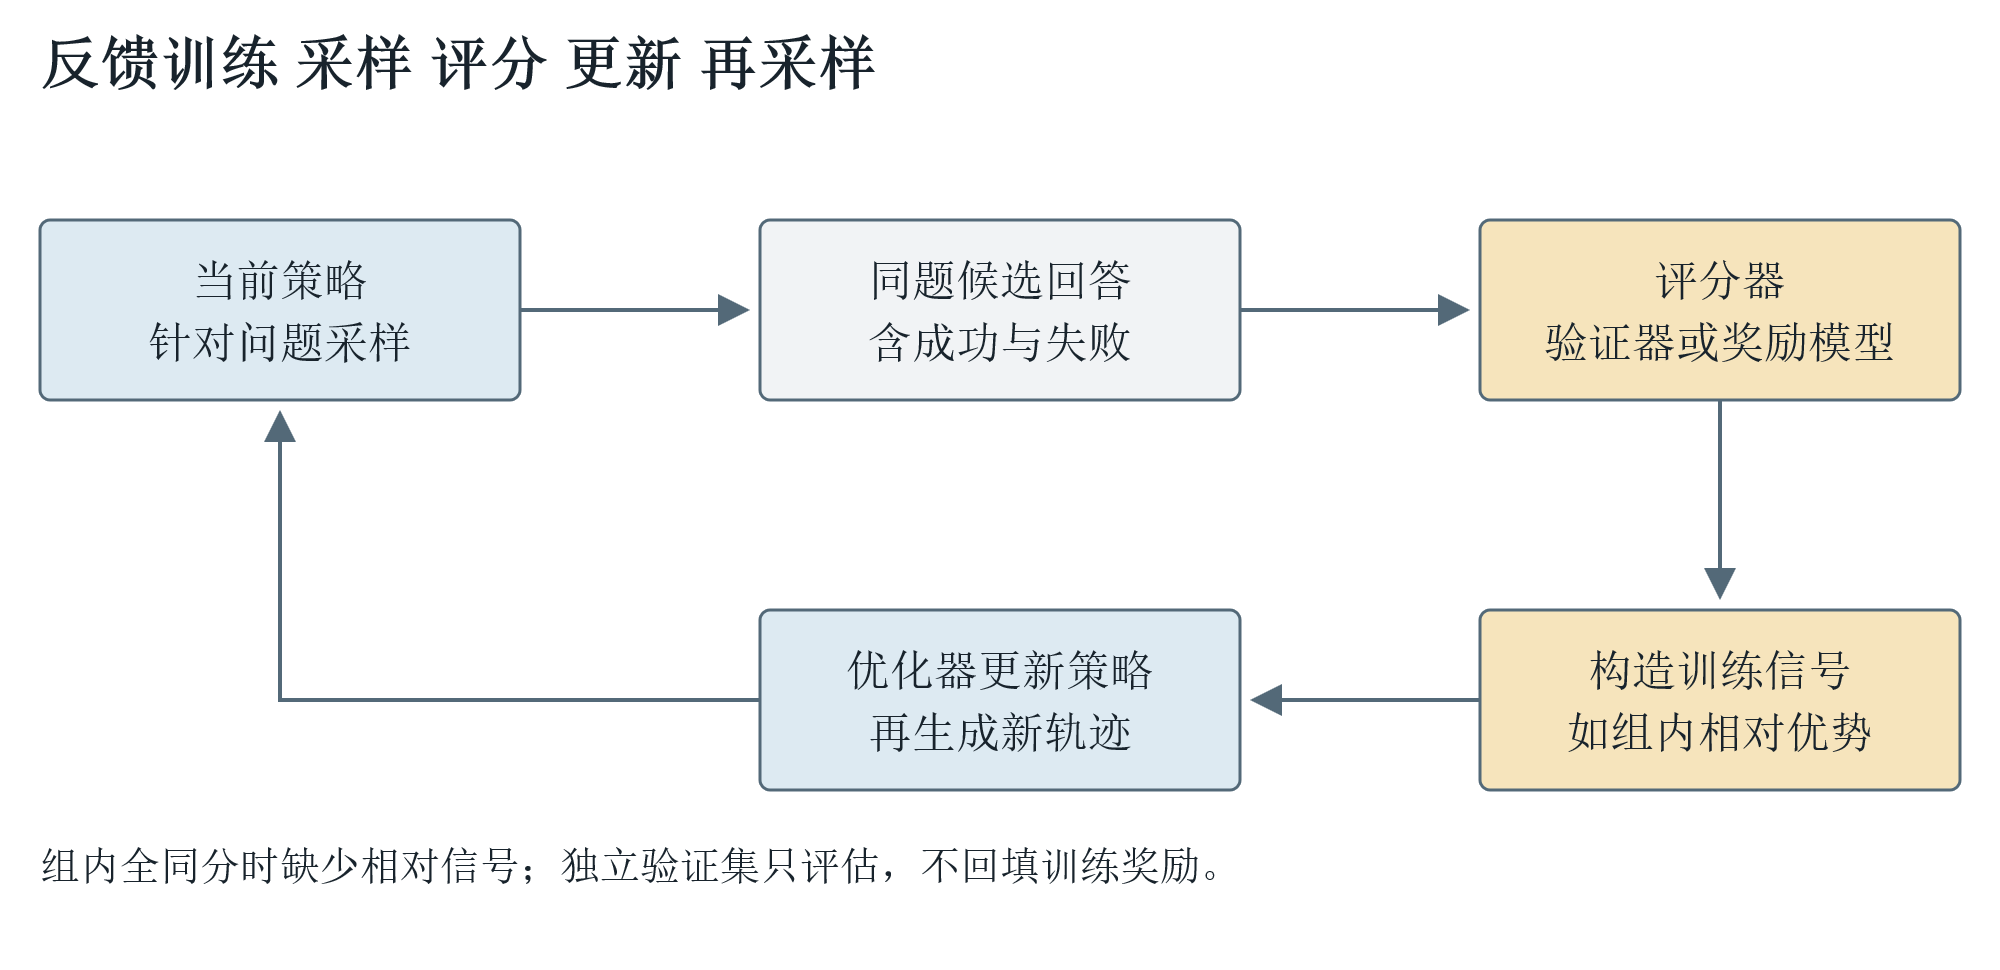
\includegraphics[width=\linewidth]{assets/media/image14.png}
    \caption{反馈训练的数据流。奖励模型与可执行验证器是两种不同评分来源；图中用组内相对优势作为后续分组比较算法的入口，不表示所有 RL 都必须采用分组比较。}
    \label{fig:反馈训练数据流}
\end{figure}

若只追求奖励最大，模型可能找到打分器的偏好捷径，例如冗长、讨好或固定套话。经典的人类反馈强化学习（Reinforcement Learning from Human Feedback，RLHF）因而常加入与参考策略的 KL 惩罚，控制偏离程度。KL 约束降低某些失控风险，却不保证真实质量；参考模型本身也可能有缺陷。 令 D 为训练问题分布、π 的下标 θ 为当前策略、π 的下标 ref 为固定参考策略，带 KL 正则且需要最大化的目标写为：
\[J(\theta) = E_{x \sim D,\, y \sim \pi_{\theta}( \cdot \mid x)}\left\lbrack r(x,y) \right\rbrack - \beta\, E_{x \sim D}D_{KL}\left( \pi_{\theta}( \cdot \mid x)\|\pi_{ref}( \cdot \mid x) \right)\]

期望符号表示对问题与生成回答求平均；第一项提高奖励，第二项扣除偏离参考策略的代价，β 是正的权衡系数。实际使用的是从采样估计的目标与梯度。

\textbf{近端策略优化（Proximal Policy Optimization，PPO）是一类策略优化方法。}本节重点介绍常见的 PPO-Clip：先用模型生成一批回答，再根据奖励估计每个生成位置的优势，最后在限制更新冲动的条件下，多次利用这批回答更新模型。``近端''可以先直观理解为：从已经采样验证过的策略附近出发，小步调整，再重新采样，这样确保参数更新是稳健的而非破坏性的。由于 PPO 算法非常重要，下面详细介绍。由于本材料尚未准备清晰的图示，强烈建议读者参考学习\href{https://datawhalechina.github.io/easy-rl/#/chapter5/chapter5}{蘑菇书}\footnote{https://datawhalechina.github.io/easy-rl/\#/chapter5/chapter5}中对 PPO 的更详细推导和图解，这也是笔者入门时的重要参考资料。

\subsection{把生成回答写成策略优化问题}

设问题为 $x$，模型生成的回答为 $y=(y_1,\ldots,y_N)$，$N$ 是本次回答的 token 数。在第 $t$ 步，状态和动作分别是：
\[
    s_t=(x,y_{<t}),\qquad a_t=y_t,\qquad
    \pi_\theta(a_t\mid s_t)=p_\theta(y_t\mid x,y_{<t}).
\]
状态就是``题目加上已经写出的内容''，动作就是下一个 token。$\theta$ 表示正在训练的语言模型参数。一次完整回答的概率是各步条件概率的乘积，取对数后则变成求和：
\[
    \pi_\theta(y\mid x)=\prod_{t=1}^{N}\pi_\theta(a_t\mid s_t),
    \qquad
    \log\pi_\theta(y\mid x)=\sum_{t=1}^{N}\log\pi_\theta(a_t\mid s_t).
\]
这说明提高某段回答的概率，最终要通过改变各个生成位置的条件概率来实现。我们不需要对``采样出一个离散 token''这个操作求导，而是在采样完成后，把得到的 token 序列送回模型，计算它们的对数概率，再对这些可微的数值求导。

在不折扣后续奖励的简化情形下，策略梯度的常见估计形式为：
\[
    \widehat g
    =\widehat{\mathbb E}_{t}
    \left[\widehat A_t\nabla_\theta
    \log\pi_\theta(a_t\mid s_t)\right].
\]
这里 $\nabla_\theta$ 表示对模型参数求梯度，$\widehat{\mathbb E}_t$ 表示在采样得到的有效生成位置上求经验平均，$\widehat A_t$ 是该位置的优势估计。严格的序列回报目标可先写成对每条轨迹逐步求和、再对轨迹求平均；这里用 token 平均展示常见训练形式，变长回答采用不同平均方式会改变样本权重。实现时必须明确这个选择，并用掩码排除提示词和补齐位置。

暂时把优势看成一个已经算好的数。若它为正，梯度上升会推动这次采到的动作变得更可能；若它为负，则推动它变得更不可能。这里改变的是``在这个前缀下生成这个 token''的倾向，改变的是条件概率分布。同时，参数又是共享的，所以实际更新还会影响其他前缀，所以这种更新也不意味着给词表里的某个 token 单独加减分。

与 SFT 相比，这里的训练方向由模型自己采样后的反馈决定：SFT 提高给定示范的概率；PPO 则既可能提高一次尝试的概率，也可能降低它。问题是，什么叫``比预期更好''，以及我们应当提高或降低多少？

\subsection{从奖励到回报，再到优势}

先区分三个概念。奖励是评分器在某一步给出的反馈；回报是从当前位置往后能够得到的累计奖励；优势则把回报与该状态下的预期水平比较。用 $\rho_t$ 表示逐步奖励，可以写成：
\[
    G_t=\sum_{j=t}^{N}\gamma^{j-t}\rho_j,
    \qquad 0\leq\gamma\leq 1.
\]
$G_t$ 是从第 $t$ 步起的采样回报，$\gamma$ 是折扣因子，越小越看重近期奖励。对于长度有限、主要关心最终回答质量的语言任务，可以取 $\gamma=1$。

最简单的结果奖励可以在回答结束时给出：中间各步 $\rho_t=0$，最后一步 $\rho_N=r(x,y)$。这并不意味着中间 token 没有训练信号：最终奖励会进入前面位置的回报。但是，只有最终结果时，算法很难精确知道哪一步推理真正起了作用；统计上加强一条高回报轨迹，也不代表这条轨迹里的每一步都已被证明正确。在大模型训练中尤其如此，对一个回答序列评判哪里推理得好哪里坏是非常贵的（可能需要专家或者强模型判定），通常简化为如果最终答案是对的，那么相同的奖励分配给这个序列生成的全部 token。

前面的参考策略 KL 惩罚，也可以放进逐步奖励。为了说明一种常见做法，设 $\pi_{\mathrm{old}}$ 是采样本批回答的策略，$\pi_{\mathrm{ref}}$ 是固定参考策略，定义：
\[
    k_t=\log\frac{\pi_{\mathrm{old}}(a_t\mid s_t)}
                         {\pi_{\mathrm{ref}}(a_t\mid s_t)},
    \qquad
    \rho_t=-\beta k_t+\mathbf{1}_{\{t=N\}}\,r(x,y).
\]
$\mathbf{1}_{\{t=N\}}$ 在最后一个位置取 1，其余位置取 0。这样，任务奖励在结尾加入，而偏离参考策略的代价沿回答累积。$k_t$ 是采样动作上的对数概率比，单次取值可以为负；只有对旧策略的动作分布取期望，才得到非负的条件 KL 散度。它不是每个 token 都必然为正的``距离''。这是在采样策略处估计 KL 惩罚的一种方式，具体系统也可以采用其他估计或直接正则化。

直接用回报更新，容易受到题目难度和奖励波动影响。价值模型（value model，也称 critic）因此学习 $V_\phi(s_t)$：在这个前缀下，按照相应策略继续生成，预期还能获得多少累计奖励。$\phi$ 是价值模型的参数。一个直观的优势估计是：
\[
    \widehat A_t=G_t-V_{\phi_{\mathrm{old}}}(s_t).
\]
$V_{\phi_{\mathrm{old}}}$ 表示更新前用来估计基线的价值模型。若实际回报是 1，而模型原来预计只有 0.4，优势就是 $0.6$，这次尝试比预期好；若回报是 0，而原来预计有 0.4，优势就是 $-0.4$。因此，奖励为正不保证优势为正，奖励为零也不保证没有梯度：关键是相对于什么预期来比较。

减去基线的作用，是减少策略梯度的波动。对于精确的、只依赖状态而不依赖当前动作的基线，在对应策略的动作分布下，有：
\[
    \mathbb E_{a\sim\pi_\theta(\cdot\mid s)}
    \left[V(s)\nabla_\theta\log\pi_\theta(a\mid s)\right]
    =V(s)\nabla_\theta\sum_a\pi_\theta(a\mid s)=0.
\]
因为所有动作概率之和恒为 1，所以减去这样的基线不改变理想策略梯度的期望。实际训练还涉及价值估计误差和后续裁剪等技巧。

\subsection{GAE 怎样把结尾反馈传回前面的 token}

PPO 常用广义优势估计（Generalized Advantage Estimation，GAE），把价值模型的预测与实际奖励结合起来。先定义一步的时序差分残差：
\[
    \delta_t=\rho_t+\gamma V_{\phi_{\mathrm{old}}}(s_{t+1})
                         -V_{\phi_{\mathrm{old}}}(s_t).
\]
它比较两个数：原来对当前状态的价值预测，以及``这一步实际拿到的奖励，加上对下一状态的价值预测''。如果后者更大，就意味着这一步之后的情况比原来预计得好。正常结束时，终止状态 $s_{N+1}$ 的价值设为 0；如果只是因为采样长度上限而中断，是否需要保留下一状态的价值估计，要按任务实际情况处理。

GAE 再把后续残差加权累积：
\[
    \widehat A_t^{\mathrm{GAE}}
      =\sum_{l=0}^{N-t}(\gamma\lambda)^l\delta_{t+l},
      \qquad 0\leq\lambda\leq 1.
\]
$\lambda$ 控制我们向后看多远。取 $\lambda=0$ 时，只用当前一步残差，较依赖价值预测；取 $\lambda=1$，且轨迹完整结束时，求和会化成采样回报减去当前价值。中间取值折中了价值估计误差与长轨迹回报的波动。

来看一个只含三个生成位置的教学例子，并非真实句子的分词。设中间奖励为 0，末尾奖励为 1，$\gamma=1$，三个位置的旧价值预测依次为 $0.4,0.6,0.8$，终止价值为 0。于是：
\[
    \delta_1=0+0.6-0.4=0.2,\quad
    \delta_2=0+0.8-0.6=0.2,\quad
    \delta_3=1+0-0.8=0.2.
\]
若再取 $\lambda=1$，三个优势就是 $0.6,0.4,0.2$。结尾的成功反馈通过求和影响了前面的位置，而前缀越接近已被预计会成功的状态，结果带来的额外惊喜越小。

\subsection{概率比 为什么需要保存采样时的旧策略}

生成回答很贵，我们希望同一批轨迹能用于若干次小批量更新。但更新一次以后，当前模型就不再是生成这批回答的那个模型了，偏离了 on-policy 的目标。如果仍不加区分地反复强化旧样本，就可能让模型过度偏向这一批偶然采到的结果。所以 PPO 通过重要性采样的方法来缓解这一问题，使得稍微旧一点的策略的样本仍然可用。

PPO 保存每个采样动作在旧策略下的概率，并在更新时计算概率比。这里用 $q_t$ 表示它，避免与奖励函数 $r(x,y)$ 混淆：
\[
    q_t(\theta)
      =\frac{\pi_\theta(a_t\mid s_t)}
                   {\pi_{\mathrm{old}}(a_t\mid s_t)}
      =\exp\left(\log\pi_\theta(a_t\mid s_t)
                 -\log\pi_{\mathrm{old}}(a_t\mid s_t)\right).
\]
分子是当前正在优化的策略，分母是本批采样时的策略；在这一批数据的若干轮更新中，分母保持不变。更新开始时两者相同，所以 $q_t=1$。若同一个前缀下，采到的 token 原概率是 0.10，当前概率变成 0.12，那么 $q_t=1.2$；变成 0.08，则 $q_t=0.8$。

在固定状态上，这种比值具有重要性加权的含义：用旧动作分布采样，也能对新动作分布下的某些量做加权估计。不过，PPO 仍然使用旧策略访问到的前缀；这个单步比值没有把所有状态分布变化都完整校正。因此，下面的式子是局部的代理目标，不是对任意新策略真实长期回报的精确计算：
\[
    L^{\mathrm{ratio}}(\theta)
      =\widehat{\mathbb E}_{t}
        \left[q_t(\theta)\widehat A_t\right].
\]
在旧策略处，对概率比求导，会得到前面策略梯度中的对数概率梯度形式。问题在于，如果只最大化这个目标，正优势动作的概率可以被不断提高，负优势动作的概率也可能被过度压低。为了避免更新幅度过大导致训练崩溃，PPO-Clip 通过裁剪重要性比率的方式缓解这一问题。

\subsection{裁剪目标 只给适度改进继续加分}

PPO-Clip 最大化的核心目标是：
\[
\begin{split}
    L^{\mathrm{CLIP}}(\theta)
    =\widehat{\mathbb E}_{t}\Big[
       \min\big(&q_t(\theta)\widehat A_t,\\
       &\operatorname{clip}(q_t(\theta),1-\epsilon,1+\epsilon)
                          \widehat A_t\big)\Big].
\end{split}
\]
其中 $\epsilon>0$ 是裁剪幅度；为方便手算，下面取 $\epsilon=0.2$。$\operatorname{clip}(q,0.8,1.2)$ 把小于 0.8 的输入变为 0.8，大于 1.2 的输入变为 1.2，区间内保持原值。$\min$ 则从原始项与裁剪项中，取对优化而言更保守的那个。注意我们在\textbf{最大化}这个目标；如果代码使用梯度下降，就要对策略目标取负号。

为什么不能只保留裁剪后的那一项？因为我们希望停止奖励``沿正确方向改得过多''，同时仍然惩罚``沿错误方向越改越差''。把优势的正负分开看，含义就清楚了\footnote{建议参考\href{https://datawhalechina.github.io/easy-rl/\#/chapter5/chapter5?id=\_522\-\%e8\%bf\%91\%e7\%ab\%af\%e7\%ad\%96\%e7\%95\%a5\%e4\%bc\%98\%e5\%8c\%96\%e8\%a3\%81\%e5\%89\%aa}{蘑菇书}里面的图示}。

\textbf{正优势：值得增加概率，但不要靠无限增加同一动作来刷目标。}假设 $\widehat A_t=0.6$，旧概率为 0.10，当前概率升到 0.13，则 $q_t=1.3$。原始项是 $1.3\times0.6=0.78$，裁剪项是 $1.2\times0.6=0.72$，最终取 0.72。概率已经沿鼓励方向提高得较多，再提高也不会让这个样本的直接策略目标继续增加。反过来，若当前概率降到 0.07，$q_t=0.7$，目标会取 $0.7\times0.6=0.42$，而不是裁剪项 0.48：正优势动作被压低这种不利变化，仍会被目标反映出来。

\textbf{负优势：值得降低概率，但也不要一次压得太狠。}假设 $\widehat A_t=-0.4$，旧概率仍为 0.10，当前概率降到 0.07，则原始项是 $0.7\times(-0.4)=-0.28$，裁剪项是 $0.8\times(-0.4)=-0.32$，最终取更小的 $-0.32$。对于最大化目标而言，从 $-0.4$ 提高到 $-0.32$ 已是改进；继续把概率压低，不再获得这一项的额外收益。若概率反而升到 0.14，目标会取 $1.4\times(-0.4)=-0.56$，继续惩罚把较差动作变得更可能的方向。

在优势固定、只考察单个位置时，同一个目标也可以写成：
\[
    \ell_t(\theta)=
    \begin{cases}
      \widehat A_t\min(q_t(\theta),1+\epsilon),
          & \widehat A_t\geq 0,\\
      \widehat A_t\max(q_t(\theta),1-\epsilon),
          & \widehat A_t<0.
    \end{cases}
\]
这揭示了裁剪的方向性：正优势主要限制过大的概率提升，负优势主要限制过大的概率压低。它不是把任何方向的变化都一律抹平。

还要避免一个常见误解：裁剪的是目标中的概率比，\textbf{不是执行一个硬约束，保证所有概率比始终落在 $[0.8,1.2]$ 内}。多个位置共享参数，其他位置的梯度、价值损失或其他正则项，仍可能把某个位置推到区间之外。裁剪也不能保证奖励每轮上升。因此还需要监控新旧策略的 KL、概率比、学习率和更新轮数；有的实现会在偏离过大时提前结束本批更新。

\subsection{价值模型怎样训练，四种模型各管什么}

策略模型需要优势，优势又依赖价值估计，所以价值模型也要更新。一种常见的回报目标由 GAE 构造：
\[
    \widehat R_t=\widehat A_t^{\mathrm{GAE}}
                   +V_{\phi_{\mathrm{old}}}(s_t),
    \qquad
    L_V(\phi)=\frac12\widehat{\mathbb E}_t
                  \left[(V_\phi(s_t)-\widehat R_t)^2\right].
\]
$\widehat R_t$ 是这批数据中固定的训练目标，不是奖励模型给的原始分数。最小化平方误差，是让价值预测接近这批轨迹提供的回报估计。计算策略损失时，缓存的优势被当作常量，不通过它反向修改价值模型；训练价值模型时，回报目标也应停止梯度。否则，模型可能通过修改``评判自己的尺子''来降低损失，而不是按预定目标学习。

如果把策略与价值部分写进一个用于梯度下降的示意损失，可以写成：
\[
    L_{\mathrm{train}}=-L^{\mathrm{CLIP}}+c_V L_V-c_H H,
    \qquad c_V,c_H\geq0,
\]
这个示意损失用于最小化，各个符号的含义如下：
\begin{itemize}
    \item $L_{\mathrm{train}}$ 是策略与价值部分组合后的训练损失。策略参数记为 $\theta$，价值模型参数记为 $\phi$；组合损失可以写成 $L_{\mathrm{train}}(\theta,\phi)$。
    \item $L^{\mathrm{CLIP}}$ 是 PPO 的裁剪策略目标，利用新旧策略的动作概率比和优势估计，衡量策略更新是否加强了高优势动作、减弱了低优势动作。原本需要最大化 $L^{\mathrm{CLIP}}$，因此改用梯度下降时写成 $-L^{\mathrm{CLIP}}$。
    \item $L_V$ 是价值预测的平方误差损失，即价值模型预测 $V_\phi(s_t)$ 与固定回报目标 $\widehat R_t$ 之间的误差。$c_V\geq0$ 是价值损失的权重，控制价值误差在组合损失中的比重；$+c_VL_V$ 表示训练要降低价值预测误差。
    \item $H$ 是当前策略的平均熵，衡量动作概率分布的分散程度。$c_H\geq0$ 是熵奖励的权重；$-c_HH$ 表示在最小化组合损失时鼓励更高的策略熵，$c_H=0$ 表示不使用熵奖励。
\end{itemize}
策略熵具体计算为
\[
H(\theta)=\widehat{\mathbb E}_t\left[
-\sum_a\pi_\theta(a\mid s_t)\log\pi_\theta(a\mid s_t)
\right].
\]
这里，$t$ 表示本批轨迹中的有效生成位置；$s_t$ 是第 $t$ 步生成前的状态，在语言模型中包含问题与已经生成的回答前缀。$a$ 表示一个候选动作，在语言模型中就是候选的下一个 token；$\sum_a$ 对所有候选 token 求和，而不是只计算实际采样到的 token。$\pi_\theta(a\mid s_t)$ 是参数为 $\theta$ 的当前策略在状态 $s_t$ 下生成 token $a$ 的概率。$\log$ 是自然对数。$\widehat{\mathbb E}_t$ 表示按本批数据中的有效生成位置计算经验平均，补齐位置不参与平均；帽号表示用有限样本估计，不代表整个状态分布下的精确期望。

例如，如果下一步只有两个候选 token，概率各为 0.5，单个位置的熵为 $-2\times0.5\ln0.5=\ln2\approx0.693$；如果一个候选 token 的概率趋近于 1，另一个趋近于 0，熵就趋近于 0。因此，熵奖励鼓励保留一定的输出多样性，但高熵本身不代表回答正确。策略熵描述当前分布是否分散，参考策略 KL 描述当前分布与参考分布相差多少，两者不是同一个量。

熵项不是每个语言模型 PPO 实现都必须使用；价值裁剪、优势归一化等也属于需要另行说明的实现选择。前面若已把参考策略 KL 计入奖励，这个示意式就不再额外重复扣一次相同的 KL。

经典 RLHF 管线中的四种角色，现在可以逐一对应：
\begin{itemize}
    \item \textbf{策略模型（actor）}负责生成回答，并通过 PPO 改变生成概率。
    \item \textbf{奖励模型（RM）}对问题与完整回答评分，提供任务反馈；在这一轮策略训练中通常固定。它回答``这份回答得到多少分''。
    \item \textbf{价值模型（critic）}读取生成前缀，预测未来累计奖励，用来估计优势；它随训练更新。它回答``写到这里，接下来预计能得多少回报''，与 RM 的输入和目标都不同。
    \item \textbf{参考策略}通常是固定的 SFT 模型，提供 KL 惩罚的参照，帮助控制相对训练起点的偏离。
\end{itemize}

旧策略还承担第五种逻辑角色：它是本批数据的生成者，提供概率比的分母。它通常是每轮采样时从当前策略确定下来的快照，可以通过保存旧 log probability 等方式使用，并不意味着始终额外常驻一个完整模型。\textbf{旧策略管的是``本批更新走了多远''，参考策略管的是``相对固定起点偏了多远''。}第一轮两者可能相同，后面旧策略随采样轮次刷新，参考策略通常保持不变，所以 PPO 裁剪与参考策略 KL 不能互相替代。价值与策略也可以共享部分参数，四种角色不一定等于四套完全独立的模型副本。

\subsection{把一轮 PPO 训练连起来}

回到小助的方程题，一轮训练可以按以下顺序理解：
\begin{enumerate}
    \item \textbf{生成。}从问题集合抽取一批题，用当前策略生成回答，此时把它视为本轮旧策略。保存生成 token、有效位置掩码和旧策略对这些 token 的 log probability。
    \item \textbf{评分。}用 RM 或验证器计算任务奖励，用参考策略计算所需的 KL 信号，并取得更新前的价值预测。按预定规则构造逐步奖励，区分正常结束与长度截断。
    \item \textbf{估计优势。}从回答末尾往前计算回报或 GAE，固定本批优势与价值训练目标。此时才确定哪些位置相对预期值得加强或减弱。
    \item \textbf{更新。}把本批数据分成小批量，重新计算当前策略概率比，优化裁剪目标，同时训练价值模型。可以重复若干遍，但旧 log probability 和本批优势不会在每一步偷偷换成新值；策略偏离过大时应限制继续复用这批数据。
    \item \textbf{刷新。}用更新后的策略重新生成下一批回答，获得新的旧策略基准。持续检查独立任务质量、奖励、参考 KL、价值误差、截断率和输出重复，而不只看策略损失是否下降。
\end{enumerate}

采样配置也属于算法的一部分。前面介绍的温度与 top-p 会改变实际生成分布；如果采样时用了截断或温度变换，概率计算就必须与所声明的行为策略和训练目标相一致。不能一边用某个分布生成，一边把另一个分布的概率直接当作采样概率，却仍声称比值完成了相应的重要性校正。

最后，PPO 不要求同一道题一定同时出现成功和失败样本。即使这一批答案全错，只要回报与价值基线仍有差异，策略或价值模型也可能收到更新；但这不保证反馈足以指明正确解法。如果奖励始终相同，价值基线又准确匹配回报，基于这些回报的优势就可能接近零。下一节的 GRPO 用同题组内比较构造优势，``全对或全错时组内没有奖励差异''才是那种设置下更直接的问题。

如果任务能可靠验证，我们也可以直接用答案正确性或执行结果奖励，不必训练 RM。这通常称为可验证奖励强化学习（Reinforcement Learning with Verifiable Rewards，RLVR）。开放偏好和可验证任务都能使用强化学习；RL 也可以有过程奖励，并非天生只给结尾一次反馈。

\textbf{本节相关资料}
\begin{enumerate}
    \item Schulman 等，2017，\href{https://arxiv.org/abs/1707.06347}{Proximal Policy Optimization Algorithms} 。\textbf{PPO的开创性论文}。阅读重点：旧策略概率比、优势与裁剪分别解决什么问题。
    \item Schulman 等，2015，\href{https://arxiv.org/abs/1506.02438}{High-Dimensional Continuous Control Using Generalized Advantage Estimation}。阅读重点：时序差分残差如何构成 GAE，以及价值基线、偏差和方差之间的关系。
    \item Ziegler 等，2019，\href{https://arxiv.org/abs/1909.08593}{Fine-Tuning Language Models from Human Preferences}。阅读重点：如何把偏好奖励、参考策略约束与 PPO 接入语言模型训练。
\end{enumerate}

\section{组相对策略优化 GRPO 同题比较如何产生信号}\label{组相对策略优化 GRPO 同题比较如何产生信号}

2025 年，正当全世界都在疑惑 OpenAI 是如何给 GPT-o1 模型训练出高质量的推理链的时候，DeepSeek-R1 横空出世，结合他们早先提出的组相对策略优化（Group Relative Policy Optimization，GRPO），在数学推理任务上取得了显著进展。这个方法既大幅节约了计算资源，还能训练出非常完整的原生思维链，大幅提高模型能力。这一模型及其技术报告一时间震惊了全世界，下面我们结合 PPO 算法介绍 GRPO 算法。

前面提到， PPO 要训练价值模型，预测每个前缀后面还能得到多少回报。GRPO 换了一种取得比较基准的方式：对同一道题采样多份回答，直接用这一组回答的奖励作比较。它由 DeepSeekMath 提出，后续也用于 DeepSeek-R1 等推理模型工作。下面沿用前一节的符号，重点解释它相对于 PPO 改了什么。

\subsection{第一处改变 用同题组内比较替代价值模型}

在前面介绍的 PPO 中，我们根据逐步奖励和价值预测计算 GAE。用最简单的完整轨迹形式来概括，就是比较``实际回报''与``价值模型原来预计的回报''：
\[
    \widehat A_t^{\mathrm{PPO}}=G_t-V_{\phi_{\mathrm{old}}}(s_t).
\]
这里的基线来自一个需要学习的函数。它可以随前缀变化：同一道题刚开始写，以及已经完成关键推导时，对成功的预期并不一样。代价是要保存、运行和训练价值模型，而且价值估计不准也会影响优势。

GRPO 在常见的结果奖励设置中，不再预测每个前缀的价值。设同一个问题 $x$ 的 $G$ 份回答是 $y_1,\ldots,y_G$，由本轮旧策略采样得到，各自奖励为 $r_1,\ldots,r_G$。先计算组内均值和标准差：
\[
    \overline r=\frac1G\sum_{i=1}^{G}r_i,
    \qquad
    \sigma_r=\sqrt{\frac1G\sum_{i=1}^{G}(r_i-\overline r)^2}.
\]
再把第 $i$ 份回答的优势写为：
\[
    \widehat A_i=\frac{r_i-\overline r}{\sigma_r+\delta},
    \qquad \delta>0.
\]
这里明确采用除以 $G$ 的总体标准差，$\delta$ 是防止除零的小常数，与 PPO 裁剪幅度 $\epsilon$ 不同。直觉上，我们把``比模型原来预计的好多少''，换成``比同一道题的其他尝试好多少''。均值提供比较基准，除以标准差则对优势尺度做归一化。

例如四份回答的奖励是 $(0,1,1,0)$。均值为 $0.5$，标准差也为 $0.5$，忽略很小的 $\delta$ 后，优势约为：
\[
    (\widehat A_1,\widehat A_2,\widehat A_3,\widehat A_4)
      =(-1,1,1,-1).
\]
同一道题内，两份成功回答受到加强，两份失败回答受到抑制。我们只需要生成与评分，就能构造这组优势，因此省去了这里的价值模型、GAE 计算和价值损失。

\subsection{第二处改变 从逐位置优势变成整段回答的相对分数}

PPO 的 GAE 会结合各个前缀的价值预测，得到可能随位置变化的 $\widehat A_t$。对于这里只在结尾评分的 GRPO，同一份回答的所有有效生成位置使用同一个优势：
\[
    \widehat A_{i,t}=\widehat A_i,
    \qquad t=1,\ldots,N_i,
\]
其中 $N_i$ 是第 $i$ 份回答的长度。也就是说，只要这份回答比组内平均更好，它采到的各个 token 都沿着加强概率的方向参与更新；比组内平均更差，则沿相反方向参与。

这种做法简化了训练，却没有精确解决步骤归因。若一份答案碰巧猜对，错误推导也可能受到加强；若前半段正确、最后一步算错，前面的有效步骤也可能随整段回答受到抑制。因此，奖励是否可靠、是否需要过程检查，依然重要。这里讲的是结果监督（Outcome Reward Model，通常简称 ORM），因为；如果提供逐步奖励，GRPO 也可以构造随位置变化的优势，GRPO 本质上是通过组内差异确定优化方向，跟整段轨迹共用同一个奖励值没有必然联系。工业领域通常在答案可可靠验证的情况下用 ORM，这样成本最低。相对应的，如果要用过程监督（Process Reward Model，PRM）进行训练，GRPO 也可以在每个位置使用不同的奖励和优势，但 PRM 的尝试大多成本高且效果不佳。

\subsection{保留的部分 概率比与 PPO 裁剪仍然存在}

GRPO 并不是算完组内分数后，直接拿成功回答再做一次 SFT。它仍然计算当前策略相对采样旧策略的概率比：
\[
    q_{i,t}(\theta)=
    \frac{\pi_\theta(y_{i,t}\mid x,y_{i,<t})}
         {\pi_{\mathrm{old}}(y_{i,t}\mid x,y_{i,<t})}.
\]
这里比 PPO 多了一个回答编号 $i$，概率比本身的意义没有改变。把前一节的裁剪项记为：
\[
\begin{split}
    C_{i,t}(\theta)=\min\big(&q_{i,t}(\theta)\widehat A_i,\\
       &\operatorname{clip}(q_{i,t}(\theta),1-\epsilon,1+\epsilon)
                        \widehat A_i\big).
\end{split}
\]
正优势不再鼓励过大的概率提升，负优势不再鼓励过大的概率压低，含义与 PPO 相同。旧策略仍需在本批更新中固定，训练后也仍要用新策略重新采样。因此，GRPO 替换的关键是优势的来源。

\subsection{第三处改变 KL 可以单独放进优化目标}

在前一节展示的 PPO 实现里，参考策略的 KL 惩罚被折算进逐步奖励，再进入回报与 GAE。DeepSeekMath 原始 GRPO 的写法则把 KL 作为目标中的独立惩罚，使组内优势由任务奖励构造。

为把含义写清楚，我们先用每个前缀上的完整词表 KL 表示正则项：
\[
    K_{i,t}(\theta)=\sum_a\pi_\theta(a\mid s_{i,t})
       \log\frac{\pi_\theta(a\mid s_{i,t})}
                     {\pi_{\mathrm{ref}}(a\mid s_{i,t})},
    \qquad s_{i,t}=(x,y_{i,<t}).
\]
$a$ 遍历下一个 token 的候选。它比较的是当前策略与参考策略在同一个前缀上的动作分布，不是当前策略与旧策略的概率比。一个便于对照的 GRPO 目标写为：
\[
    J_{\mathrm{GRPO}}(\theta)=
      \mathbb E_{\substack{x\sim D,\\
                  y_{1:G}\sim\pi_{\mathrm{old}}(\cdot\mid x)}}
      \left[\frac1G\sum_{i=1}^{G}\frac1{N_i}
         \sum_{t=1}^{N_i}\left(C_{i,t}(\theta)-\beta K_{i,t}(\theta)\right)
      \right].
\]
外层期望表示对题目和旧策略生成的回答组求平均；$1/G$ 对回答求平均；$1/N_i$ 对一份回答内部的有效位置求平均。第一项根据组内优势和裁剪更新策略，第二项限制偏离参考策略。公式这里是完整词表 KL，实际上浪费了大量计算资源，因为绝大部分 token 的概率都几乎为 0，可以用 top-k 选择头 k 个 token 重新计算概率分布然后计算 KL 散度。$\beta$ 是 KL 惩罚系数，通常在训练中保持不变。

这种按回答再按长度平均的写法，让每份回答先形成一个平均贡献，而不是天然让长回答因 token 多而获得更大总权重。但不同的长度归一化会改变优化偏好，不能把长度处理当作无关紧要的细节。后续变体可能调整它、去掉组内标准差缩放，或者改变 KL 设置；GRPO 公认的改进包括 DAPO，GSPO 等，都是在这个基础上做的。

这里对比的是两种具体写法，并不是说 PPO 必须把 KL 放进奖励、GRPO 永远必须单独加 KL。无论采用哪种算法，旧策略仍然是采样与裁剪的基准，参考策略仍然提供偏离惩罚的参照。

\subsection{高熵 token 为什么值得重点训练}

前面的策略目标把每个有效生成位置都纳入更新。进一步的问题是：一段推理中的所有位置，对学会解题贡献是否相同？有些位置主要延续熟悉的词语与格式，有些位置则面对多种合理续写，选择之后会进入不同的推理路径。识别后面这类位置，可以帮助我们把训练信号集中到更有选择空间的决策点。

\textbf{高熵描述一个位置的候选分布}~在第 $i$ 份回答的第 $t$ 个生成位置，用采样时的旧策略计算熵：
\[
H_{i,t}=-\sum_{v\in\mathcal V}
\pi_{\mathrm{old}}(v\mid s_{i,t})
\log\pi_{\mathrm{old}}(v\mid s_{i,t}).
\]
这里，$i$ 是回答编号，$t$ 是回答中的生成位置，$s_{i,t}$ 是问题与此前已生成 token 构成的前缀，$\mathcal V$ 是词表，$v$ 遍历候选 token。$\pi_{\mathrm{old}}(v\mid s_{i,t})$ 是采样策略对候选 token 的条件概率，$\log$ 是自然对数，因此 $H_{i,t}$ 的单位为 nat。概率集中在少数候选上时，熵较低；多个候选都有较大概率时，熵较高。文献把高熵位置上生成的 token 简称为高熵 token，熵的计算对象是生成前的完整候选分布。

例如，假设某个位置只有两个候选，概率为 $(0.99,0.01)$，熵约为 0.056 nat；另一个位置的候选概率为 $(0.5,0.5)$，熵约为 0.693 nat。第二个位置有更大的选择空间。单个已采样 token 的惊讶度则是 $-\log\pi_{\mathrm{old}}(y_{i,t}\mid s_{i,t})$，其中 $y_{i,t}$ 是实际生成的 token。即使分布很集中，偶尔采到概率为 0.01 的候选也会得到较高惊讶度；按熵筛选时仍使用该位置的整个分布。

\textbf{为什么这些位置可能影响推理方向}~例如，模型写到``接下来采用''时，可以继续代入、分类讨论或反证，不同续写会改变后续求解过程；已经选定公式后，固定表达中的部分 token 则较容易预测。对于已经掌握基本语言与解题表达的模型，强化学习可以重点调整前一类选择：利用成功轨迹提高有效分支的概率，利用失败轨迹降低低收益分支的概率。熵提供候选位置，奖励与优势提供更新方向；正优势加强该位置实际采取的选择，负优势减弱该选择。

\textbf{怎样在损失里选择训练位置}~一种实现方式是根据采样批次中有效生成位置的熵确定阈值 $\tau$，保留熵最高的一部分位置，定义固定掩码
\[
m_{i,t}=\mathbf 1[H_{i,t}\geq\tau],\qquad
J_{\mathrm{select}}(\theta)=
\frac1G\sum_{i=1}^{G}\frac1{N_i}
\sum_{t=1}^{N_i}m_{i,t}C_{i,t}(\theta).
\]
这里，$m_{i,t}$ 是位置选择掩码，$\mathbf 1[\cdot]$ 在条件成立时取 1，否则取 0；$\tau$ 是熵阈值，例如按有效位置的熵分位数选取最高的 20\%。$G$ 是同题回答数，$N_i$ 是第 $i$ 份回答的有效生成长度，$C_{i,t}(\theta)$ 是前面定义的裁剪策略目标，$\theta$ 是当前策略参数。这个示意式沿用按完整回答长度归一化的方式，只展示策略更新项；KL 正则仍按具体训练配置单独组织。熵与掩码在本批更新中作为固定的选择依据，梯度通过保留位置的策略目标计算。

当 $m_{i,t}=0$ 时，该位置不直接贡献策略目标；整段回答仍参与生成，也作为后续位置的上下文。注意力连接使保留位置的梯度能够通过前缀计算传播，共享参数更新后，各个位置的输出分布也会随之改变。选择性训练因此减少了直接参与策略目标的位置，完整的采样与前向计算仍承担轨迹生成和熵统计的工作。

\textbf{实验支持了什么}~Wang 等人在 2025 年的《Beyond the 80/20 Rule》中研究了基于可验证奖励的强化学习（Reinforcement Learning with Verifiable Rewards，RLVR）。在其 Qwen3 推理训练实验中，仅保留熵最高的 20\% 位置的策略梯度，在 8B 模型上取得与全位置训练相当的表现，在 14B 和 32B 模型上取得更高表现；只训练熵最低的 80\% 位置则明显退化。论文报告，32B 模型在 AIME 2025 上相对全位置训练提高约 11.04 个百分点。这组对照支持把训练重点放在高熵决策位置的做法。

在训练诊断中，可以同时记录逐位置熵、选中比例和独立题集成绩，并比较全位置、高熵位置、低熵位置与随机位置四种更新方式。由此可以判断当前模型的收益来自哪些位置，选择合适的保留比例，并把策略更新集中到更有效的推理决策上。

\subsection{省下什么，又付出什么}

从训练流程看，原来的``采样、评分、预测价值、计算 GAE、更新策略与价值模型''，变成了``同题多次采样、评分、计算组内优势、更新策略''。价值模型的前向计算、反向传播及相应参数和优化器状态可以省去，但同一道题现在要生成多份回答。在固定总生成 token 预算下，分给一题的尝试越多，本批能够覆盖的不同题目就可能越少。PPO 也可以对同题多次采样，区别在于这里的组内比较直接依赖这些样本。

组内比较还带来一个明确限制。若四份回答全错，奖励都是 0，则组内均值是 0，标准差也是 0，加上 $\delta$ 后优势仍全为 0；若四份全对且奖励相同，优势也全为 0。这一组没有从结果奖励中产生相对策略信号，所以没有任何优化效果。相比之下，PPO 即使遇到相同奖励，也可以因为价值预测与回报不同而产生非零优势。

即使组内优势为零，独立 KL 正则也仍可能有梯度，所以不能说模型参数一定不变。若大量题目都产生零方差组，我们应检查题目是否过难或过易、奖励是否过于粗糙、采样是否缺乏差异。

标准差缩放也会影响题目之间的权重。例如四份回答只有一份成功，奖励为 $(0,0,0,1)$，均值为 $0.25$，标准差为 $\sqrt{3}/4$；忽略 $\delta$，唯一成功回答的优势约为 $1.73$，每份失败回答约为 $-0.58$。它们与两对两错时的 $\pm1$ 不同。可见，归一化不只是方便显示分数，也实际改变了各条轨迹的更新权重，仍需要结合题目分布评估。

回到小助，GRPO 的主要变化可以归结为：用同题的实际尝试构造比较基准，省去学习价值函数的环节，同时保留带裁剪的策略更新。我们因此除了看平均奖励，还要看每题成功率、零方差组比例、输出重复率、截断率和长度分布。只有这些信号一起改善或者保持，才能判断省下价值模型后，采样和比较是否仍在有效推动学习。

\textbf{本节相关资料}
\begin{enumerate}
    \item Shao 等，2024，\href{https://arxiv.org/abs/2402.03300}{DeepSeekMath Pushing the Limits of Mathematical Reasoning in Open Language Models}。阅读重点：第 4.1 节如何替换价值基线、保留裁剪目标，以及区分结果监督与过程监督的优势构造。
    \item DeepSeek-AI 等，2025，\href{https://arxiv.org/abs/2501.12948}{DeepSeek-R1 Incentivizing Reasoning Capability in LLMs via Reinforcement Learning}。阅读重点：GRPO 如何与奖励、冷启动及多阶段训练配合，避免把模型效果全部归因于单个算法。
    \item Wang 等，2025，\href{https://arxiv.org/abs/2506.01939}{Beyond the 80/20 Rule: High-Entropy Minority Tokens Drive Effective Reinforcement Learning for LLM Reasoning}。阅读重点：逐位置生成熵、高熵位置策略梯度掩码，以及与全位置和低熵位置训练的对照。
\end{enumerate}

\section{直接偏好优化 DPO 为什么可以绕过奖励模型}\label{直接偏好优化 DPO 为什么可以绕过奖励模型}

假如我们已经收集了``同一题，两份回答，哪份更好''的数据。PPO 路线先把它们变成奖励模型，再在线采样更新策略。我们自然会问：能否直接像对比学习一样用偏好对训练模型，少维护一个奖励模型？直接偏好优化（Direct Preference Optimization，DPO）就从这个问题进入，正如其论文名称所说：``你的大语言模型本身就是一个隐藏的奖励模型''。

\textbf{先读懂最优策略公式}~策略就是模型面对问题 \(x\) 时，对不同回答 \(y\) 分配的概率。参考策略 \(\pi_{ref}\) 是一份冻结的基准模型，通常取偏好训练开始前的 SFT 模型。先假设奖励 \(r(x,y)\) 已经给定，带 KL 正则的目标是：
\[
\max_{\pi}\;\mathbb{E}_{y\sim\pi(\cdot\mid x)}[r(x,y)]
-\beta D_{KL}\bigl(\pi(\cdot\mid x)\|\pi_{ref}(\cdot\mid x)\bigr),\qquad\beta>0.
\]
第一项鼓励多生成高奖励回答，第二项惩罚过度偏离参考分布的行为。在归一化和支持等条件下，这个目标的最优策略为
\[
\pi^*(y\mid x)=\frac{\pi_{ref}(y\mid x)e^{r(x,y)/\beta}}{Z(x)},
\qquad Z(x)=\sum_y\pi_{ref}(y\mid x)e^{r(x,y)/\beta}.
\]
可以把它分成三步读：先取参考概率，再乘以奖励带来的放大倍数 \(e^{r/\beta}\)，最后除以所有回答的加权概率之和，使新概率加起来仍等于 1。奖励越高，相对放大越多；在奖励固定时，\(\beta\) 越大，放大倍数之间的差异越弱，最优策略越接近参考策略。

例如，暂时假设只有两份候选回答，参考概率各为 0.5。若偏好回答的奖励为 \(\beta\ln3\)，偏恶回答的奖励为 0，那么放大倍数分别为 3 和 1，归一化后概率就从 \((0.5,0.5)\) 变为 \((0.75,0.25)\)。这里用给定奖励解释最优分布；DPO 的关键是反过来利用这个关系，让偏好标签直接训练策略，无需先获得这些数值奖励。

我们把它反过来整理，奖励可以表示成策略与参考策略的对数概率比，再加一个只依赖问题 x 的项。拿同一道题的两个答案相减时，这个项消失。于是，偏好概率能直接写成策略概率的函数，不必另训显式奖励网络。 对上式取对数并整理，把奖励改写成策略概率比，得到：
\[r(x,y) = \beta log\frac{\pi^{*}(y \mid x)}{\pi_{ref}(y \mid x)} + \beta logZ(x)\]

β log Z(x) 只依赖问题，不依赖回答。因此，同一道题的两个奖励相减时，这一项恰好抵消；不是在所有计算中都可以直接丢掉它。

为了看清损失，我们定义一个差值 Δ：被偏好回答相对参考的对数概率增量，减去不被偏好回答的对应增量。若 Δ 越大，模型就越符合这条偏好。DPO 用负对数 sigmoid 拟合标签。 沿用同一问题 x 与正负回答的记号，差值 Δ 的定义为：
\[\Delta_{\theta} = log\frac{\pi_{\theta}\left( y^{+} \mid x \right)}{\pi_{ref}\left( y^{+} \mid x \right)} - log\frac{\pi_{\theta}\left( y^{-} \mid x \right)}{\pi_{ref}\left( y^{-} \mid x \right)}\]

每个比值都把当前策略与同一个参考策略比较；Δ 先计算正回答的相对增量，再减去负回答的相对增量。

再把这个差值代入偏好概率，对偏好数据取负对数似然，DPO 损失写为：
\[L_{DPO} = - E_{\left( x,y^{+},y^{-} \right)}log\sigma\left( \beta\Delta_{\theta} \right)\]

损失中的 \(E_{(x,y^+,y^-)}\) 表示对偏好数据集中的样本取平均；每个样本由问题 \(x\)、偏好回答 \(y^+\) 和偏恶回答 \(y^-\) 组成。\(\sigma\) 是 sigmoid 函数，定义为 \(\sigma(z)=1/(1+e^{-z})\)，把实数 \(z\) 映射到 0 与 1 之间。\(\beta>0\) 是前面 KL 正则目标中的权重系数，在 DPO 损失中乘在对数概率比差值 \(\Delta_\theta\) 前，控制 sigmoid 输入的尺度。\(\theta\) 表示当前模型的可训练参数；训练通过最小化 \(L_{DPO}\) 的梯度更新 \(\theta\)，参考模型的参数保持冻结。

\textbf{偏好回答与偏恶回答怎样推动更新}~对同一个问题 \(x\)，标注者较喜欢的回答记为 \(y^+\)，较不喜欢的回答记为 \(y^-\)。偏恶表示本次比较中较差，不代表它的每句话都错。例如，用户要求解释一道题，偏好回答 \(y^+\) 给出正确推导，偏恶回答 \(y^-\) 在关键一步用了错误规则。数据提供的是``回答 \(y^+\) 优于回答 \(y^-\)''的标签，而不是两份回答各自的数值奖励。

把前面的差值合并，就能看出 DPO 直接比较的量：
\[
\Delta_\theta
=\log\frac{\pi_\theta(y^+\mid x)}{\pi_\theta(y^-\mid x)}
-\log\frac{\pi_{ref}(y^+\mid x)}{\pi_{ref}(y^-\mid x)}.
\]
也就是说，当前模型对偏好回答与偏恶回答的概率比，应当比参考模型的相应概率比更高。这里的 \(\log\) 均为自然对数。采用 Bradley--Terry 偏好模型时，获胜概率由奖励差的 sigmoid 给出；代入反解出的奖励，便得到
\[
P_\theta(y^+\succ y^-\mid x)=\sigma(\beta\Delta_\theta),
\qquad\sigma(z)=\frac{1}{1+e^{-z}}.
\]
这个概率是对``哪份回答会胜出''的预测，不是生成 \(y^+\) 本身的概率。单对样本的损失为 \(\ell_\theta=-\log\sigma(\beta\Delta_\theta)\)。差值增大，预测的获胜概率就升高，损失就降低。

用便于计算的假想序列概率演示：参考模型对两份回答的概率分别为 0.2 和 0.1，概率比为 2。当前模型从参考模型初始化时，\(\Delta_\theta=0\)，预测获胜概率为 0.5，损失约为 0.693。若训练后概率变成 0.3 和 0.05，概率比便从 2 提高到 6，此时
\[
\Delta_\theta=\ln\frac{0.3/0.05}{0.2/0.1}=\ln3.
\]
为方便演示取 \(\beta=1\)，则 \(\sigma(\ln3)=0.75\)，损失降为 \(-\ln0.75\approx0.288\)。这组数字展示损失鼓励的变化方向，并非一次更新必然得到的结果。

\begin{figure}[t]
    \centering
    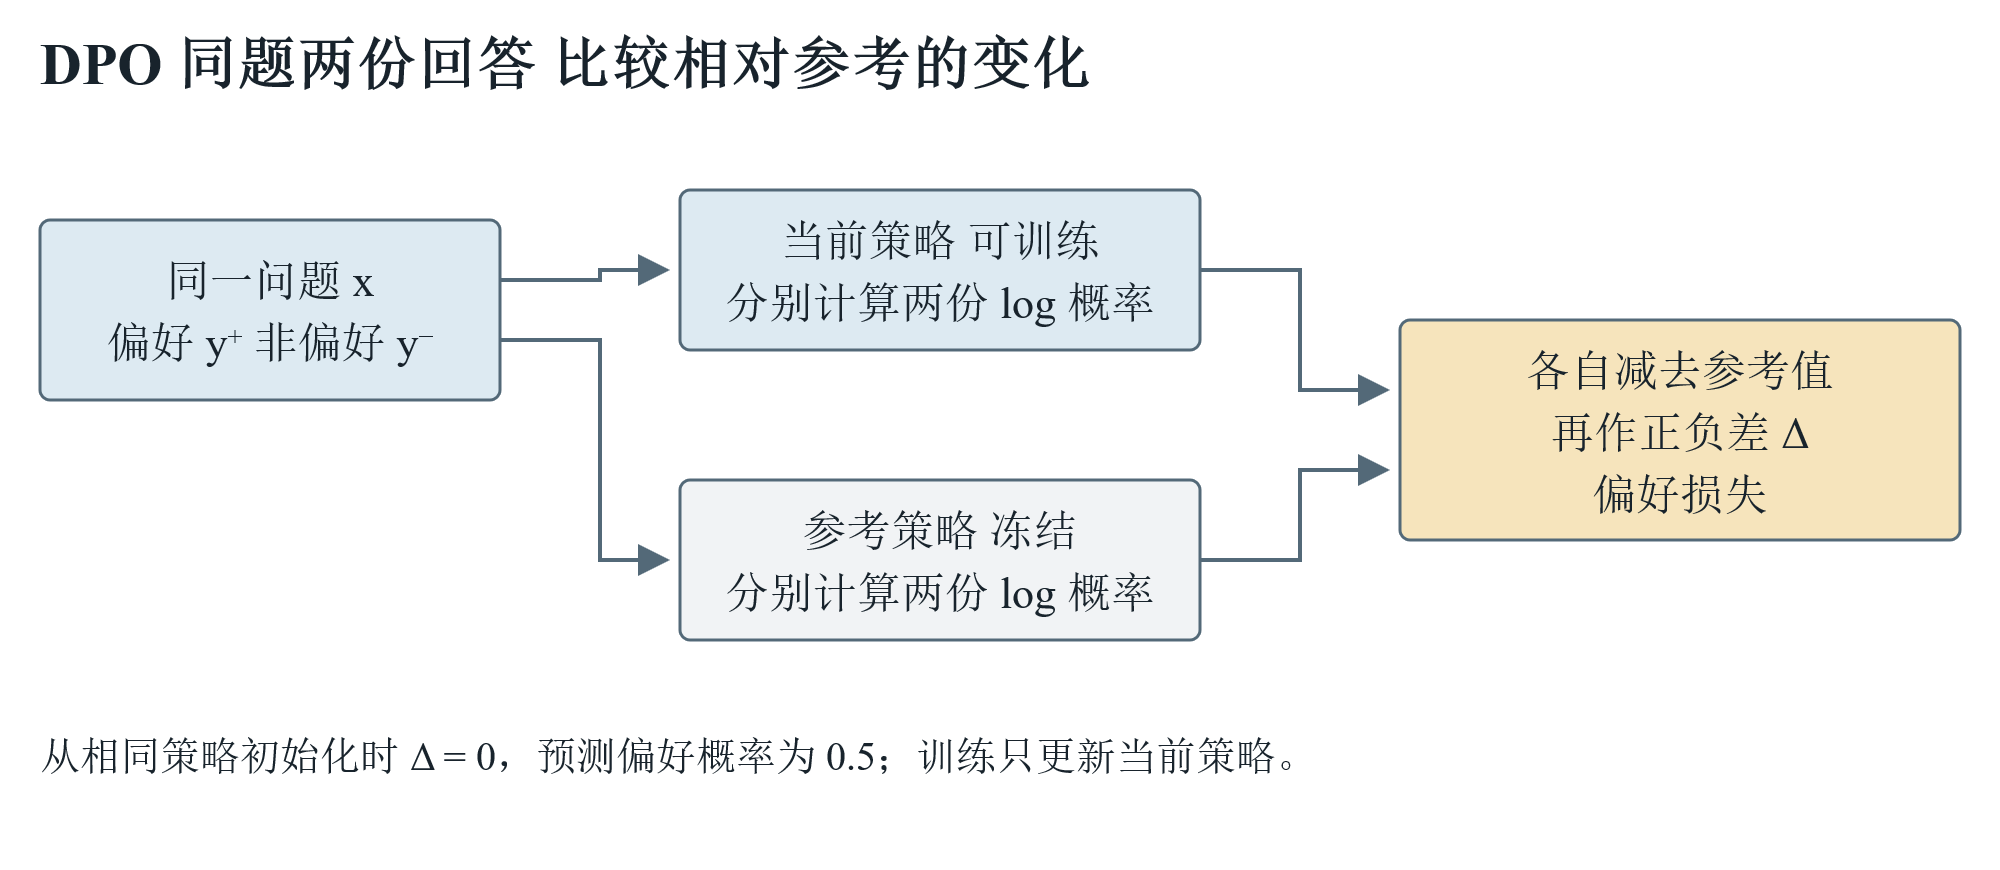
\includegraphics[width=\linewidth]{assets/media/image16.png}
    \caption{DPO 的比较对象。参考策略参与计算但不随本次损失更新；梯度只更新当前策略。离线数据是否覆盖当前行为，需要在下一节另行检查。}
    \label{fig:DPO比较对象}
\end{figure}

进一步看单对样本的梯度，就能看到两份回答如何共同提供训练信号。参考模型保持冻结，有
\[
\nabla_\theta\ell_\theta
=-\beta\sigma(-\beta\Delta_\theta)
\left[\nabla_\theta\log\pi_\theta(y^+\mid x)
-\nabla_\theta\log\pi_\theta(y^-\mid x)\right].
\]
梯度下降要减去这个梯度，因此更新方向包含提高偏好回答对数概率的方向，以及降低偏恶回答对数概率的方向。前面的权重会在模型尚未符合这对偏好时较大，在模型已经明显拉开差距时较小。两份回答共用网络参数，实际不能保证每一步都让前者的绝对概率上升、后者的绝对概率下降；目标直接约束的是它们相对参考模型的概率比。

回答的对数概率又是逐 token 对数概率之和：
\[
\log\pi_\theta(y\mid x)
=\sum_{t=1}^{|y|}\log\pi_\theta(y_t\mid x,y_{<t}).
\]
因此，偏好信号最终通过这些 token 的对数概率反向传播到模型权重。许多偏好对一起调整生成分布，让类似输入下的行为更符合标注偏好。能否推广到新问题，仍取决于数据覆盖与模型泛化；序列级标签也不会自动指出偏恶回答究竟错在哪个 token。

这里用的是回答序列的概率，实际通过 token log probability 加总计算，通常不把提示文本（prompt）对应的 token 计入回答概率。长短答案、截断、补齐掩码（padding mask）和模板仍会影响结果。它与 SFT 一样可以 teacher forcing 计算给定回答的概率，但损失还比较正负回答和与参考模型的偏离程度，并非等价于 SFT。

我们把四次概率计算画在图 \ref{fig:DPO比较对象}：两份回答分别经过当前策略与冻结参考策略。先减参考，再比较正负，才能得到前面定义的 Δ。

我们用一个小例子观察参考的作用。假如训练策略从参考初始化，最初每份回答的对数概率比都为零，Δ 也为零，对这对样本预测偏好概率为 0.5。训练再根据标签拉开相对差异。若标签总偏爱长答案，模型也可能学到长度捷径。

DPO 的理论联系建立在偏好建模与理想化优化条件上。有限数据、受限模型族和分布外输入，会使实际行为偏离理想。我们获得的是一种直接优化方式，仍然需要训练和独立评估。

\textbf{实践}~用 DPO 方法训练一个小模型，观察它在训练集和独立评估集上的行为，比如有一些开源项目训练原始模型为网店客服的语言风格。

\textbf{本节相关资料}
\begin{enumerate}
    \item Rafailov 等，2023，\href{https://arxiv.org/abs/2305.18290}{Direct Preference Optimization Your Language Model is Secretly a Reward Model}。\textbf{提出 DPO 方法的论文}。阅读重点：从最优策略关系反解奖励，以及为什么归一化项在偏好比较中抵消。
    \item Azar 等，2023，\href{https://arxiv.org/abs/2310.12036}{A General Theoretical Paradigm to Understand Learning from Human Preferences} 。阅读重点：偏好建模和优化目标的假设怎样影响方法选择。
\end{enumerate}

\section{离线与在线偏好优化 数据如何跟上策略}\label{离线与在线偏好优化 数据如何跟上策略}

我们用同一份偏好集做了许多轮 DPO。训练集的偏好分类越来越容易，实际对话却出现一类新错误：模型在较长的解释中反复自我肯定。旧偏好数据里没有这种回答，我们也从未评价过它。此时，问题从``如何拟合标签''转为``标签覆盖了谁的行为''。

离线偏好优化把已有回答当作固定训练材料。我们不需要在每个优化步骤在线生成，成本容易控制，数据也便于审核。可当策略（也就是模型行为）发送明显变化，静态样本未必覆盖新模型常生成的轨迹。

我们可以周期性让当前模型生成新候选，再标偏好、再优化。这是在线或迭代偏好优化的一种思路。它把反馈追到学生的新行为上，但也增加采样、评审与版本管理成本。一次收集、多轮训练与持续重采样之间存在很多中间方案，不是非此即彼。

DPO 存在许多变体方法，我们继续用三个问题定位：信号是什么，数据由谁产生，更新依赖哪些组件。恒等偏好优化（Identity Preference Optimization，IPO）研究另一类偏好目标；卡尼曼与特沃斯基优化（Kahneman--Tversky Optimization，KTO）可以使用好坏标签而不要求每条都是成对偏好；简单偏好优化（Simple Preference Optimization，SimPO）以平均序列对数概率构造无参考奖励；优势比偏好优化（Odds Ratio Preference Optimization，ORPO）把监督学习与偏好约束结合，省去独立参考模型。知道这些差别，就能理解它们各自减少了什么成本，而不急着背公式清单。

我们会先选实现清楚、数据适配的方法建立基线。当独立评估显示静态数据覆盖不足，再引入迭代收集。这个顺序使每一次复杂度增加都对应已观察到的需求。

需要注意的是，与 LoRA 一样，工业领域基础模型团队为了确保训练框架简单可靠，通常不会支持太多分支功能，因此可能也不支持 DPO 训练，因为通常可以通过强化学习解决相同问题。

\textbf{本节相关资料}
\begin{enumerate}
    \item Azar 等，2023，\href{https://arxiv.org/abs/2310.12036}{A General Theoretical Paradigm to Understand Learning from Human Preferences}，包含 IPO 。阅读重点：为何要重新检查偏好目标。
    \item Ethayarajh 等，2024，\href{https://arxiv.org/abs/2402.01306}{KTO Model Alignment as Prospect Theoretic Optimization} 。阅读重点：不成对的好坏标签怎样提供信号。
    \item Meng 等，2024，\href{https://arxiv.org/abs/2405.14734}{SimPO Simple Preference Optimization with a Reference-Free Reward} 。阅读重点：参考模型与长度处理的改变。延伸比较 ORPO：\href{https://arxiv.org/abs/2403.07691}{{原文链接}} 。
\end{enumerate}

\section{RL 泛化诊断 训练涨分而验证不涨}\label{RL 泛化诊断 训练涨分而验证不涨}

我们完成一轮 RL，训练奖励从教学案例中的 0.35 升到 0.70，验证集答案正确率却几乎不动意味着我们必须立即开始检查。

``训练涨''可能指在线生成轨迹（rollout）的奖励，也可能指固定训练题的独立评估；``验证不涨''可能指最终答案正确率，也可能指人工偏好。若前者是代理 RM 分数，后者是真实任务质量，两个指标原本就不等价。我们必须在固定训练题和验证题上，都用同一套解码预算与独立评分重评一次，把测量差异先拿掉。通常来说，我们需要同时观察 reward 曲线、rollout 准确率曲线和验证集准确率曲线。

第一种可能是记住了题目或模板。我们按原始题族切分，测试换数值、换叙述、换组合方式。若只在见过的表述上变好，继续增加同类重复题可能让曲线更漂亮，却不能支持迁移。我们应补充机制相同但表面不同的训练覆盖，并保留真正未参与开发的测试题。

第二种可能是奖励被钻空子，称为奖励黑客（reward hack）。小助把``因此答案正确''写得更频繁，RM 更喜欢，独立验证器却看不到改善。我们检查高奖励失败样本，尤其看奖励提升最大的部分。必要时修评分规范、增加反例、改验证器，再从合理检查点重训。\textbf{需要注意的是，reward hack 已经成为目前 RL 训练的最根本问题之一，理论上说，如果能根除 reward hack，那么我们可以训练出任何想要的模型能力。} Reward hack 存在许多形式，有的简单有的复杂，复杂的非常难识别和抑制，我们也许可以调用一个超强外部模型来判别，但是强化学习需要大量 rollout，大量强模型的判别的成本极高，人工专家判别则效率过低。目前，reward hack 已经成为最难解决的问题之一，这也吸引了大量研究者投入到 reward hack 的研究中。

第三种可能是训练与验证题目分布不同，就是题目之间差距太大。训练主要是一两步代数，验证集更多是长条件、多步组合。训练收益可能真实，但局限于训练集已覆盖的能力区域。我们按知识点和难度分桶，看哪些桶有迁移，再决定补数据、安排课程学习或调整目标任务。

第四种可能是评估噪声或预算变化。小评估集、随机采样、答案解析错误，都能掩盖变化。我们报告题目数和重复次数，对同一题做成对比较，必要时估计置信区间。若新模型用了更长输出或更多采样，还需观察质量与 token 成本的关系。

我们可以把证据整理为一个紧凑矩阵，再选下一步实验。

\begin{longtable}[]{@{}
  >{\raggedright\arraybackslash}p{(\linewidth - 4\tabcolsep) * \real{0.2985}}
  >{\raggedright\arraybackslash}p{(\linewidth - 4\tabcolsep) * \real{0.2985}}
  >{\raggedright\arraybackslash}p{(\linewidth - 4\tabcolsep) * \real{0.4030}}@{}}
\toprule\noalign{}
\begin{minipage}[b]{\linewidth}\raggedright
\textbf{观察}
\end{minipage} & \begin{minipage}[b]{\linewidth}\raggedright
\textbf{优先假设}
\end{minipage} & \begin{minipage}[b]{\linewidth}\raggedright
\textbf{下一步检查}
\end{minipage} \\
\midrule\noalign{}
\endhead
\bottomrule\noalign{}
\endlastfoot
训练 RM 涨 独立正确率不涨 & 奖励偏离真实目标 & 人工审查高奖励失败样本 \\
固定训练题涨 未见题不涨 & 记忆或覆盖不足 & 按题族和难度分桶重评 \\
答案更长 得分差异不稳定 & 预算或测量混淆 & 固定 token 与采样预算 \\
一个题型涨 另一个题型降 & 收益不均或能力干扰 & 分项指标与旧能力回归测试 \\
\end{longtable}

\textbf{本节相关资料}
\begin{enumerate}
    \item Gao 等，2022，\href{https://arxiv.org/abs/2210.10760}{Scaling Laws for Reward Model Overoptimization} 。阅读重点：怎样分别衡量代理目标与更可信的目标。
    \item Srivastava 等，2022，\href{https://arxiv.org/abs/2206.04615}{Beyond the Imitation Game Quantifying and extrapolating the capabilities of language models} 。阅读重点：任务多样性为何影响我们对能力的判断。
\end{enumerate}

\section{RL 训练诊断 从数据与判题检查到补回 SFT}\label{RL 训练诊断 从数据与判题检查到补回 SFT}

另一轮实验中，小助的训练奖励几乎是一条直线。我们先做一次很小的链路检查：确认官方样例或简单题能运行、参数确实更新、采样端加载了新权重、奖励方向没有写反。使用经过验证的成熟训练基础设施（infrastructure，常简称 infra）\footnote{推荐了解 Slime 和 VeRL 这两种框架，都是工业界最常用的强化学习基础设施，也推荐读者自行基于这些 infra 实践。这些 infra 本身的优化也是现代人工智能领域的重要研究课题。}，并确认关键配置后，我们把主要排查精力转向题目难度、参考答案与判题器。这是当前实验的排查顺序，不是对所有框架故障率的统计结论；有明确异常日志时，仍应沿证据检查实现。

\textbf{先看数据是否处在可学习的难度区间}~我们固定采样预算，对每题生成一组回答，查看每题成功率与同分组比例。如果绝大多数题都远超小助当前能力，组内反复全错，GRPO 就缺少有用的相对奖励信号。我们先排除错答案和误判，再适当降低题目难度、补充中间难度题或拆分子任务。全对题也不能不看覆盖需求就全部删除；目标是让当前策略有机会产生可以比较的尝试。最终纳入强化学习训练的样本，通常是正确率不那么高，但是能够采样到过程和答案都正确轨迹的题目。

\textbf{造数据时就交叉核验答案}~我们不把一个强模型生成的答案直接当作标准答案。先让多个强模型独立解题，尽量不向它们展示候选标准答案，避免互相照抄或被同一答案锚定；再把最终答案按约定格式归一化，比较是否一致。有分歧的题先复核、重写或剔除。模型之间也可能共享错误，所以一致只是筛选信号；能用计算、执行、符号检验或原始资料确认的题，应继续核验，并抽样人工检查一致通过的样本。

我们把用于自动判分的最终答案设计得简短清晰，例如一个词语、一个数值或一个短语，同时保存可核查的解题依据。数值题预先规定单位、精度与容差；词语和短语题规定合理的别名、大小写与等价表达。这里约束的是最终答案与判分接口，推理过程仍可按任务需要保留。题目本身也要避免条件缺失、多解却只登记一个答案等问题。

\textbf{把判题器当作需要验收的组件}~我们用已知正确、已知错误及边界样本测试判题规则。例如``5''\,``5.0''\,``a＝5''是否应当等价，要由这道题的答案规范决定；``5 米''不能在量纲不符时仅因含有数字 5 就得分。我们检查答案抽取、等价判断、单位、超时和空输出，再抽样复核真实 rollout。假阴性样本会让有效尝试拿不到奖励，假阳性样本则可能让模型学会利用判题漏洞。

\textbf{优先构造短答案题，谨慎使用选择题}~选择题让模型可以通过猜测、排除或选项中的表面线索得分，而不必完成我们希望训练的求解。因此，在能够可靠判分时，我们优先让小助直接给出词语、数值或短语，而不是把训练题默认做成四选一。猜中本身不等于奖励投机，但持续利用选项位置、措辞或解析漏洞，会使奖励与实际求解能力脱离。

如果任务必须使用单选题，我们可以把候选数扩展到 10 项，条件允许时再试 20 项，并保证干扰项有意义、题目仍有唯一正确答案。在完全均匀盲猜且只有一个正确选项时，命中率分别是 10\% 和 5\%；这不是实际模型的猜测率保证。无效干扰项容易被排除，增加选项还会增加输入长度与阅读难度，因此要比较这些变化后的真实收益。

在造题目时，我们可以为每次 rollout 独立打乱选项顺序，并同时重建显示标签与正确答案映射。稳定保存每个选项的内容标识、排列和随机种子，判题时先把模型选择映射回实际内容，再与标准答案比较。若只打乱选项却沿用原来的字母答案，反而会制造错误奖励；``以上皆是''等依赖位置的表述也须先改写。

排查完数据与判题，再看温度、生成长度、KL 约束、学习率、优势与裁剪：输出是否过度重复，是否被截断，更新是否过弱？我们一次改一个因素。若干净题目和可靠判题都已确认，而模型在可接受预算内仍反复缺少关键步骤，再用经审核的针对性 SFT 示范建立起点。补完以后，先检验留出题，再观察是否出现更多有效尝试与组内差异，最后重启 RL。

我们在示范与反馈之间按证据往返。成熟链路做简短确认，数据难度、答案与判题做重点复核；补 SFT 的依据通常是 rollout 尝试全部失败，都出现关键过程或者结果错误。

还有一点需要了解的是，强化学习仅仅训练少量专用数据也几乎不会造成灾难性遗忘，这与 SFT 截然不同。

\textbf{本节相关资料}
\begin{enumerate}
    \item Pezeshkpour 与 Hruschka，2023，\href{https://arxiv.org/abs/2308.11483}{Large Language Models Sensitivity to The Order of Options in Multiple-Choice Questions} 。阅读重点：选项排列如何影响测量；正文中的 10 或 20 项与逐次打乱是需要在具体任务中验证的工程建议，并非该论文给出的通用最优配置。
\end{enumerate}

\chapter{知识蒸馏~从教师示范到同策略学习}\label{知识蒸馏}

第五章介绍了用奖励或偏好优化模型行为。本章转向另一种训练信号：让学生模型学习教师模型提供的回答或概率分布。知识蒸馏（Knowledge Distillation，KD）把教师的行为迁移给学生，常用于降低部署成本、培养领域能力和传递推理方法。教师可以是更大的通用模型，也可以是某个任务上更强的专家模型。

理解蒸馏可以围绕两个问题：教师提供什么信号，学生在哪些前缀上学习。教师可以提供完整回答，也可以提供下一 token 的概率；训练前缀可以来自教师示范，也可以来自学生当前生成的轨迹。这两个选择共同决定数据构造、损失计算和教师接口的要求。

\section{序列蒸馏~把教师回答变成训练数据}\label{序列蒸馏}

最直接的方式是准备一组问题，让教师生成回答，经检查与筛选后，把问题和教师回答组成 SFT 数据。学生使用教师强制学习目标序列，其训练方法与第四章相同，区别在于目标回答由教师模型提供。只取得文本回答的教师接口就可以支持这条路线，不同分词器的学生可以按自己的词表重新编码回答。

例如，教师为一道方程题生成条件整理、移项与求解步骤，检查器确认结果后，将完整解答交给学生训练。学生学习解题顺序、表达方式和目标答案。收集短答案、完整推导或工具调用轨迹，分别对应不同的行为目标；数据中的长度、难度和任务比例也会影响学生学到的行为。

这条路线通常先生成固定数据，再多轮训练学生，称为离线序列蒸馏。实践中可以为同题生成多个候选，结合执行结果和人工抽查保留高质量示范，再混合原有任务数据训练。训练后分别检查新任务成绩、原有能力与回答成本，选择适合部署的学生版本。

\section{分布蒸馏~学习教师对候选 token 的判断}\label{分布蒸馏}

如果教师接口能够提供下一 token 概率，学生就可以学习整个候选分布。例如，同一个前缀下，教师给三个候选分配 $(0.7,0.2,0.1)$，这份信号既指出首选，也保留了其他续写的相对可能性。对齐这些概率需要教师与学生在同一前缀上预测，并把候选事件对应起来。

一种基础目标是正向 KL：
\[
L_{\mathrm{KD}}(\theta;h)=
D_{\mathrm{KL}}\bigl(\pi_T(\cdot\mid h)\|\pi_\theta(\cdot\mid h)\bigr)
=\sum_{v\in\mathcal V}\pi_T(v\mid h)
\log\frac{\pi_T(v\mid h)}{\pi_\theta(v\mid h)}.
\]
这里，$h$ 是选定的生成前缀，$\pi_T$ 是固定教师的下一 token 分布，$\pi_\theta$ 是参数为 $\theta$ 的学生分布，$\mathcal V$ 是对齐后的共同候选词表，$v$ 遍历候选 token，$\log$ 是自然对数。$L_{\mathrm{KD}}$ 衡量学生与教师在该前缀上的分布差异，训练时再对样本和有效生成位置取平均。优化器更新学生参数，教师保持固定。

直接逐 token 比较时，使用相同分词器与词表最便于对齐；跨词表蒸馏则需要额外构造片段或序列级的对应关系。实际选择还取决于能否获得完整概率、可用带宽和教师前向计算成本。序列蒸馏以教师给出的回答为目标，分布蒸馏则进一步利用候选之间的相对概率。

\textbf{基础阅读}
\begin{enumerate}
    \item Hinton、Vinyals 与 Dean，2015，\href{https://arxiv.org/abs/1503.02531}{Distilling the Knowledge in a Neural Network}。阅读重点：教师概率分布作为训练目标，以及知识迁移与模型压缩的联系。
\end{enumerate}

\section{同策略蒸馏 OPD~让老师反馈学生轨迹}\label{同策略蒸馏 OPD 让老师反馈学生轨迹}

前面的分布蒸馏还需要选择计算反馈的前缀。同策略蒸馏（On-Policy Distillation，OPD）让学生先生成回答，再由教师在学生实际经过的前缀上提供反馈。它把教师指导放到学生自身的生成路径上，可以复用强化学习中的采样和策略更新组件。

模型的错误通常发生在推理轨迹中间某一步。单个最终奖励告诉它``没有做对''，却未必指出从哪个分叉开始偏离；照抄老师的完整解答又主要覆盖老师走过的前缀。我们于是尝试另一种教学安排：学生先自己走，老师在学生走到的位置上给反馈。

OPD 不是 2025 年才突然出现的单一算法，但是直到 2025 年才被广泛关注；广义知识蒸馏（Generalized Knowledge Distillation，GKD）与 MiniLLM 等工作已经研究过相关思路；MiniLLM 是方法名称。不同实现可以使用不同散度、不同轨迹混合与不同梯度估计。我们先理解共同结构，再选一种反向 KL 形式作例子。

在学生生成的前缀 h 上，老师和学生各给出下一 token 分布。反向 KL 把学生分布放在期望的采样侧：学生常选择、老师却不支持的 token，会产生较大的平均代价。若能取得完整分布，就可以对词表求和。 把老师策略记为 π 的下标 T，在同一个学生前缀 h 上，反向 KL 定义为：
\[D_{KL}\left( \pi_{\theta}\|\pi_{T} \mid h \right) = \sum_{v}^{}\pi_{\theta}(v \mid h)\log\frac{\pi_{\theta}(v \mid h)}{\pi_{T}(v \mid h)}\]

求和的 v 遍历词表，θ 表示学生参数；两边必须在同一前缀下给概率。该式是词表分布的 KL，不是单个 token 的人类正确性标签。

若只查询学生实际采样 token 的 log probability，可以用对数概率差构造随机估计，并把相反方向的差作为逐 token 反馈。单个采样差值可以为负，KL 的非负性指的是分布期望；``红色 token''也不自动等于人类语义上确定错误的步骤。 把第 t 步学生前缀记为 h 的下标 t、采样动作记为 a 的下标 t，用老师与学生的对数概率差构造反馈：
\[{\widehat{r}}_{t} = log\pi_{T}\left( a_{t} \mid h_{t} \right) - log\pi_{student}\left( a_{t} \mid h_{t} \right)\]

π 的下标 student 表示用于反馈计算的学生策略，帽号提示这是基于采样的信号。实际实现要说明使用采样时还是更新时的概率，以及哪些量停止梯度。

学生已经走错时，老师面对的是错误前缀。老师可能纠正它，也可能只给出在错误前提下自然的延续。于是，分布反馈很密集，却不等于可靠的步骤真值。通常来说，OPD 方法有效的前提是学生轨迹仍在老师的（正确轨迹）覆盖范围内，允许有一些小偏差。若学生的分布与老师的分布差异过大，则可能收效甚微。

关于正向 KL 散度和反向 KL 散度，我们把两个 KL 方向放回同一幅图景。正向 KL 从老师分布出发，通常更强调覆盖老师的多种模式；反向 KL 从学生分布出发，在受限模型族等条件下常表现出更强的模式选择倾向。本材料讲的相对简略，网络上有许多详细讲解可参考，比如\href{https://zhuanlan.zhihu.com/p/1996277720846471471}{关于正反KL散度}\footnote{https://zhuanlan.zhihu.com/p/1996277720846471471}。

Thinking Machines 在 2025 年的\href{https://thinkingmachines.ai/blog/on-policy-distillation/}{研究博客}\footnote{https://thinkingmachines.ai/blog/on-policy-distillation}中展示了推理与个性化的 OPD 实验，并用采样 token 的老师 log probability 构造密集反馈。低 KL 说明学生接近老师，不能保证接近事实真相；老师的错误、风格偏差与盲点仍会传递。

回到续训退化，我们可以让学生在真实任务前缀上向保留良好行为的老师学习。但老师若没有新课程知识，就不能指望它凭空教会学生。实际还要考虑 tokenizer 对齐、概率接口是否可用、老师计算成本与数据覆盖。OPD 把反馈带到学生路径上，成功条件仍要通过实验确认。

到这里，读者应该自然理解这个教师模型必须与学生模型有完全一样的词表，否则 logits 无法对应训练，也就无法计算 KL 散度，而不同家族的模型词表几乎都是不同的。若老师是黑箱模型，只能给出最终回答，学生就无法在自己的轨迹上逐 token 获得反馈。有了 OPD 也不意味着就可以在任意情况下轻松通过蒸馏把一个弱模型训练成强模型，因为我们首先要有一个同源的强模型，这个强模型通常通过前面的传统方法（SFT 和 RL）训练得到。

那么还有一个问题，如果我们已经有了这个强模型，直接用这个模型不就可以了，为什么还要蒸馏一个小模型呢？原因在于，例如我们要训练一个数学专家模型，准备了一批数学领域的优质 SFT 和 RL 数据，这批数据要与其他领域的许多数据混合以训练一个通用强模型，在这个数据混合的过程中可能存在数据模式冲突，导致类似``1+1<2''的情况出现。但是有了 OPD，我们就不需要关注除了数学以外其他领域的能力，只需要让模型在数学领域成为专家；同样的，其他领域也可以有这种专家模型，然后再通过 OPD 把这些专家模型作为混合教师，蒸馏到一个模型上，这样数据模式冲突的情况就会被规避掉，实践表明这的确收益更高。

\textbf{思考问题}~如果老师是一个黑箱模型，只能给出最终回答，是否还有其他方法实现 OPD？

\textbf{本节相关资料与研究材料}
\begin{enumerate}
    \item Agarwal 等，2023，\href{https://arxiv.org/abs/2306.13649}{On-Policy Distillation of Language Models Learning from Self-Generated Mistakes}，GKD 。阅读重点：学生生成的数据与不同散度目标。
    \item Gu 等，2023，\href{https://arxiv.org/abs/2306.08543}{MiniLLM: On-Policy Distillation of Large Language Models} 。阅读重点：反向 KL 与自回归蒸馏中的优化问题。
    \item Kevin Lu 与 Thinking Machines，2025，\href{https://thinkingmachines.ai/blog/on-policy-distillation/}{https://thinkingmachines.ai/blog/on-policy-distillation/}，\textbf{OPD 最重要的研究博客}。阅读重点：采样 token 反馈的实现与实验条件；它不是普适效率保证。
\end{enumerate}

\section{后训练方法比较 依据信号与分布作选择}\label{后训练方法比较 依据信号与分布作选择}

结合第四章的监督微调、第五章的奖励与偏好优化，以及本章的知识蒸馏，可以按训练信号和轨迹来源选择方法。DPO 使用回答之间的偏好标签，蒸馏使用教师示范或概率反馈；两者分别围绕偏好学习与教师行为迁移组织训练。

我们用三个轴定位：信号从哪里来，轨迹由谁产生并多久更新，优化需要维护什么组件。信号成本也不一定单调下降，老师前向、人工标注与规则验证的价格取决于场景。

\begin{longtable}[]{@{}
  >{\raggedright\arraybackslash}p{(\linewidth - 6\tabcolsep) * \real{0.1567}}
  >{\raggedright\arraybackslash}p{(\linewidth - 6\tabcolsep) * \real{0.2537}}
  >{\raggedright\arraybackslash}p{(\linewidth - 6\tabcolsep) * \real{0.3209}}
  >{\raggedright\arraybackslash}p{(\linewidth - 6\tabcolsep) * \real{0.2687}}@{}}
\toprule\noalign{}
\begin{minipage}[b]{\linewidth}\raggedright
\textbf{方法}
\end{minipage} & \begin{minipage}[b]{\linewidth}\raggedright
\textbf{主要训练信号}
\end{minipage} & \begin{minipage}[b]{\linewidth}\raggedright
\textbf{轨迹或数据来源}
\end{minipage} & \begin{minipage}[b]{\linewidth}\raggedright
\textbf{更新方式}
\end{minipage} \\
\midrule\noalign{}
\endhead
\bottomrule\noalign{}
\endlastfoot
SFT & 目标回答 token & 人类或老师等外部示范 & 最大似然 \\
拒绝采样 RFT & 筛过的成功回答 & 当前或旧检查点采样 & 筛选后最大似然 \\
PPO 类 RL & 结果或过程回报 & 当前或近期策略采样 & 带约束的策略梯度 \\
GRPO 类 RL & 组内相对回报 & 同题多次策略采样 & 相对优势更新 \\
离线 DPO & 被偏好与不被偏好回答 & 固定偏好数据 & 直接偏好损失 \\
OPD & 老师概率或分布 & 学生轨迹或混合轨迹 & 散度或相应梯度估计 \\
\end{longtable}

我们据此决定下一步。若新行为连一条可靠示范都没有，先建设 SFT 示范轨迹数据；若成功路径可采到且可验证，选择 RFT 或者 RLVR 路线；若有明确偏好对但在线训练成本受限，可以选择 DPO 方法；若有现成的强老师模型和可用概率接口，可以考虑 OPD。若问题只是缺少最新课规，回到 RAG，不必先更新权重。

如果读者学完并且基本完全理解了前面的所有内容，那么就已经可以称为是大模型后训练方面的专家了。

\begin{figure}[t]
    \centering
    
\includegraphics[width=0.7\linewidth]{assets/media/吴恩达-机器学习专家.jpg}
    \caption{你已经成为大模型后训练方面的专家}
\end{figure}

\chapter{推理策略与推理时计算}\label{推理策略与推理时计算}

\section{思维链 CoT 与推理时计算}\label{思维链 CoT 与推理时计算}

训练告一段落，我们给小助一道需要多步转换的题。让它直接报答案时容易出错；让它先列出条件、写中间计算，再给结论，成功率可能提高。我们没有更新权重，却给了它更多生成过程。这就是思维链（Chain-of-Thought，CoT）与推理时计算（test-time compute）的入口。

自回归模型每生成一个 token，都进行一次依赖此前内容的计算。中间文字可以记录变量、拆解子问题、保留暂时结果，因此延长序列有时相当于把计算展开到更多步骤。但可见解释不是对内部机制的完整读出，模型也可能先偏向一个答案，再写出似乎合理的说明。我们评估步骤是否有效，不把流畅的长解释当成真实正确的证明。

我们还可以并行多试几次，再用选择器挑选。若题目有可规范化的最终答案，可以多数投票，这就是 self-consistency 的常见用法。它利用不同采样路径在答案上的一致性，却要求正确答案能形成足够支持。若模型反复犯同一种系统错误，多数投票反而会稳定选错。

另一种方式是多候选择优（best-of-N）：生成 N 个候选，由验证器或奖励模型选最好的。投票不需要评估每条步骤质量，选择器则可以利用更多信息，但会受到自身误差影响。若训练奖励曾被钻空子，那么验证器就需要改进。

我们把三种方案放在相同预算下比较：一条长解答、几条短解答、多候选加验证。难题可能值得更多计算，简单题则无需长篇推导。若把更长输出全部视为进步，就会忘记用户需要的是及时而可靠的帮助。真正的曲线应当是任务质量相对于总 token、延迟和计算成本的变化。

训练 scaling 改变模型能力与分布，推理时计算则在给定模型上分配更多尝试或过程。它们可以互相补充，也可能受到不同瓶颈限制。模型若缺少必需知识，多想一会儿未必能补出来；若只是算术容易失误，调用计算器可能比再推理一千个 token 更有效。

\textbf{本节相关资料}
\begin{enumerate}
    \item Wei 等，2022，\href{https://arxiv.org/abs/2201.11903}{Chain-of-Thought Prompting Elicits Reasoning in Large Language Models} 。阅读重点：示例中的中间步骤如何影响任务表现。
    \item Wang 等，2022，\href{https://arxiv.org/abs/2203.11171}{Self-Consistency Improves Chain of Thought Reasoning in Language Models} 。阅读重点：多样采样与答案聚合的分工。
    \item Snell 等，2024，\href{https://arxiv.org/abs/2408.03314}{Scaling LLM Test-Time Compute Optimally can be More Effective than Scaling Model Parameters} 。阅读重点：推理预算如何随问题难度分配。
\end{enumerate}

\section{推理模型 从示范和结果反馈到蒸馏}\label{推理模型 从示范和结果反馈到蒸馏}

观察到``多写步骤有时有用''，不等于模型已经学会稳定推理。小助可能把每题都写得很长，却重复同一句话；也可能在关键处跳步。看起来像思考的轨迹不如有效的推理行为。有时候我们需要更细的监督信号，帮助模型学会在更多题上稳定地写出有效步骤，但这非常困难。

示范路线提供高质量解题轨迹，让学生学习分解、求解和检查；反馈路线让模型自己尝试，再依靠可验证结果或过程评价改进；蒸馏路线把强模型的解题数据或分布反馈交给较小学生。它们可以串联，也可以在不同阶段交替。对一个薄弱起点，先给有效示范常能改善后续探索；对已有丰富能力的起点，直接 RL 也可能发现新的有效行为。

DeepSeek-R1-Zero 的实验探索了从基座直接进行大规模 RL 的路线；R1 则使用冷启动数据和多阶段训练，处理可读性、语言一致性等需求。我们阅读时区分研究问题：前者展示特定起点与奖励条件下直接 RL 的可能性，后者展示面向更完整助手行为的组合管线。但是 GRPO 训练也不能保证模型自动就学会推理，这取决于答案是否可验证，在多大程度上确保了过程合理性，以及奖励模型的能力和偏差。

过程监督可以更细地评价中间步骤，结果监督则通常更容易自动获得。前者需要可靠的步骤标签或评审，后者可能把偶然猜中当成成功。我们可以抽查``答案正确但理由无效''和``中间合理但最后算错''两类样本，理解不同信号各自漏掉什么。

小模型学习强模型时，也有两种不同蒸馏。把老师完整解答做成数据再 SFT，是离线序列蒸馏；让学生自己生成、再查询老师分布，是第六章介绍的 OPD。长推理过程蒸馏并不天然等于 OPD。学生若模仿了复杂措辞却无法执行其中步骤，说明数据难度、表示能力或优化还需要调整。

我们还会遇到 thinking 与 non-thinking 模式。具体角色标记、开关和停止规则由模型定义，不能把某个产品接口当成所有模型的标准。实验时记录实际模板、是否允许生成推理段、推理预算与答案抽取方式；否则同一个模型也可能因为入口不同呈现完全不同的表现。


\section{工具调用推理 让模型在行动与反馈中求解}\label{工具调用推理}

小助遇到一道新任务：读取一份销售表，计算各地区的同比增长率，再找出增长最快的地区。完成任务需要取出文件中的数据、执行数值计算，并把结果整理成解释。工具调用推理把这些步骤连接起来：模型决定下一步需要什么信息或计算，向外部工具发出请求，读取工具返回的结果，然后继续求解。搜索、数据库、代码解释器、计算器和文件读取器，都可以成为这个过程中的工具。

\subsection{一次工具调用怎样发生}

工具调用需要模型与执行程序配合。执行程序向模型提供工具名称、功能说明、参数格式和返回内容的约定；模型据此选择工具，并生成结构化调用请求。执行程序读取请求、运行相应工具，再把执行结果写回对话上下文。模型读取新增结果后，决定继续调用还是生成最终答案。

以计算增长率为例，假设系统提供一个名为 \texttt{calculator} 的工具，接收字符串参数 \texttt{expression}。模型可以生成如下请求：
\begin{verbatim}
{"name": "calculator",
 "arguments": {"expression": "(125-100)/100*100"}}
\end{verbatim}
执行程序把表达式交给计算器，得到 25，再把返回值作为工具结果交给模型。模型据此解释``销售额从 100 增加到 125，同比增长 25\%''。工具名称决定调用哪个程序，参数决定程序具体计算什么，返回值提供后续回答使用的数值。结构化请求由模型生成，数值运算由计算器完成，结果解释由模型继续生成。

每次调用还可以附带调用标识，用来把返回结果与对应请求配对。执行程序通过工具结果消息将返回值交给模型，模型便能区分自己提出的操作和工具实际返回的信息。对于文件检索，返回结果可以包含文件名与段落位置；对于代码执行，返回结果可以包含标准输出、错误信息和生成文件的位置。

\subsection{从一次计算到多轮推理}

回到销售表任务，小助可以按以下顺序求解：
\begin{enumerate}
    \item \textbf{读取数据。}调用文件工具取得列名与数据，确认地区、年份、销售额和单位。例如，甲地区两年的销售额为 100、125，乙地区为 80、112，单位均为万元。
    \item \textbf{确定计算。}采用同比增长率公式 $(\text{本年销售额}-\text{上年销售额})/\text{上年销售额}$，把地区与年份对应到正确的数据列。
    \item \textbf{执行计算。}调用代码工具计算两个地区的增长率，得到甲地区 25\%、乙地区 40\%，并按增长率排序。
    \item \textbf{处理反馈。}如果工具返回缺失列或非数值字段，小助根据报错检查列名与数据格式，调整读取或计算请求，再次执行。
    \item \textbf{组织答案。}根据返回结果指出乙地区增长最快，并列出两个地区的原始销售额、增长率和计算口径。
\end{enumerate}
每一次工具返回都会改变模型下一步能够利用的信息。读取文件后，模型知道实际有哪些字段；运行代码后，模型得到计算值；遇到错误后，模型获得修改下一次请求的依据。推理因而形成``判断下一步、执行操作、读取反馈、更新判断''的循环。

ReAct 将推理与行动交替组织：推理帮助选择和调整行动，行动从外部环境取得新观察。在工具调用系统中，模型可以用简短计划决定下一次操作，执行程序负责把操作落实到具体工具。读者可以通过调用请求与返回结果追踪求解过程：模型查了什么、算了什么，以及最终答案使用了哪些结果。

\subsection{用公式表示行动与观察}

把第 $t$ 轮调用前的历史记为 $h_t$，模型的下一次操作记为 $a_t$，工具返回的观察记为 $o_t$，工具交互可以写成：
\[
    a_t\sim\pi_\theta(\cdot\mid h_t),\qquad
    o_t=\mathcal T(a_t),\qquad
    h_{t+1}=\operatorname{append}(h_t,a_t,o_t).
\]
这里，$t$ 表示交互轮次；$h_t$ 包含用户问题、工具说明以及此前的调用与结果；$\theta$ 是模型参数；$\pi_\theta(\cdot\mid h_t)$ 是模型基于历史生成下一次操作的条件分布。$a_t$ 包含所选工具及其参数，$\sim$ 表示从模型分布生成操作。$\mathcal T$ 表示执行工具的外部程序，$o_t$ 表示本次实际返回的内容；搜索工具的返回还取决于查询时的数据状态。$\operatorname{append}$ 表示把调用和结果追加到历史，形成下一轮输入 $h_{t+1}$。模型在信息足够时生成最终答案，结束交互。

模型仍然逐 token 生成内容，只是生成内容现在包含工具名称、参数和控制调用的结构。工具执行期间，外部程序完成检索、运算或环境操作；工具返回后，模型在扩充的上下文上继续生成。在一次推理会话中，工具结果通过上下文改变后续输出，模型参数保持固定。

\subsection{工具使用怎样训练，计算预算怎样分配}

监督微调可以使用包含工具说明、调用参数、执行结果和最终答案的完整交互轨迹。模型学习在什么位置调用、选择哪个工具、怎样填写参数，以及怎样利用返回内容。训练时，工具返回内容作为上下文提供；损失通常计算在需要模型生成的调用与回答位置，使模型学习控制求解过程。Toolformer 研究了自动构造和筛选工具调用数据的路线：保留有助于后续文本预测的调用，再用筛选后的数据训练模型。

强化学习则可以让模型在工具环境中完成任务，并根据最终结果与调用成本获得反馈。沿用第五章的策略优化思路，动作现在可以是一段代码、一次检索请求或一个计算表达式。任务完成奖励推动模型选择有效操作，调用次数和执行时间的成本推动模型减少重复操作。训练轨迹保留工具返回与后续修正，模型便能从交互结果学习连续决策。

推理时的计算预算也随之扩展：除了生成多少 token，还要决定检索多少次、执行多少段代码，以及哪些操作可以并行。两个互不依赖的资料查询可以同时发出；需要读取文件后才能确定的计算请求，则按数据依赖顺序执行。面对销售表任务，一次代码执行可以完成所有地区的计算和排序，把模型的生成预算留给列名理解、口径选择与结果解释。

工具调用还会增加上下文中的文件片段、执行日志和中间结果。执行程序可以返回与当前决策相关的摘要、数据片段或输出文件位置，让模型保留任务所需的证据与状态。随着交互轮数增加，这些新增内容也进入后续推理的计算与存储成本，接下来讨论的 KV 缓存正承担着保存这些历史状态的工作。

\textbf{本节相关资料}
\begin{enumerate}
    \item Yao 等，2022，\href{https://arxiv.org/abs/2210.03629}{ReAct: Synergizing Reasoning and Acting in Language Models}。阅读重点：推理、行动与外部观察怎样交替构成求解过程。
    \item Schick 等，2023，\href{https://arxiv.org/abs/2302.04761}{Toolformer: Language Models Can Teach Themselves to Use Tools}。阅读重点：工具调用数据的生成、筛选与训练方式。
\end{enumerate}

\section{KV 缓存与推理服务 长上下文的资源成本}\label{KV 缓存与推理服务 长上下文的资源成本}

现在小助终于能认真解题，却让服务器变慢了。我们没有改参数，显存仍然迅速增长。原因之一是每个会话在生成过程中保留了越来越长的键值缓存（Key--Value Cache，KV Cache），后文简称 KV 缓存。

推理可分为预填充（prefill）和逐步解码（decode）。prefill 处理输入前缀，计算各层 key 与 value；decode 每轮生成一个新 token，查询此前缓存。缓存复用历史位置已经算好的 K、V，减少重复计算。解码时，当前查询仍需要读取历史键值；随着上下文增长，每一步的读取量与注意力计算量也随之增加。

图 \ref{fig:KV缓存复用} 接回第二部分的 QKV：进入新位置后，我们计算这个位置的新 Q、K、V；新 Q 读取缓存中的历史键值以及当前位置键值，完成注意力，再将当前位置 K、V 追加进缓存。历史位置在因果模型中不受后续 token 影响，因此相同前缀下可复用这些历史状态。这里画的是逐位置的数据依赖，具体算子可以把追加与读取融合执行。

\begin{figure}[t]
    \centering
    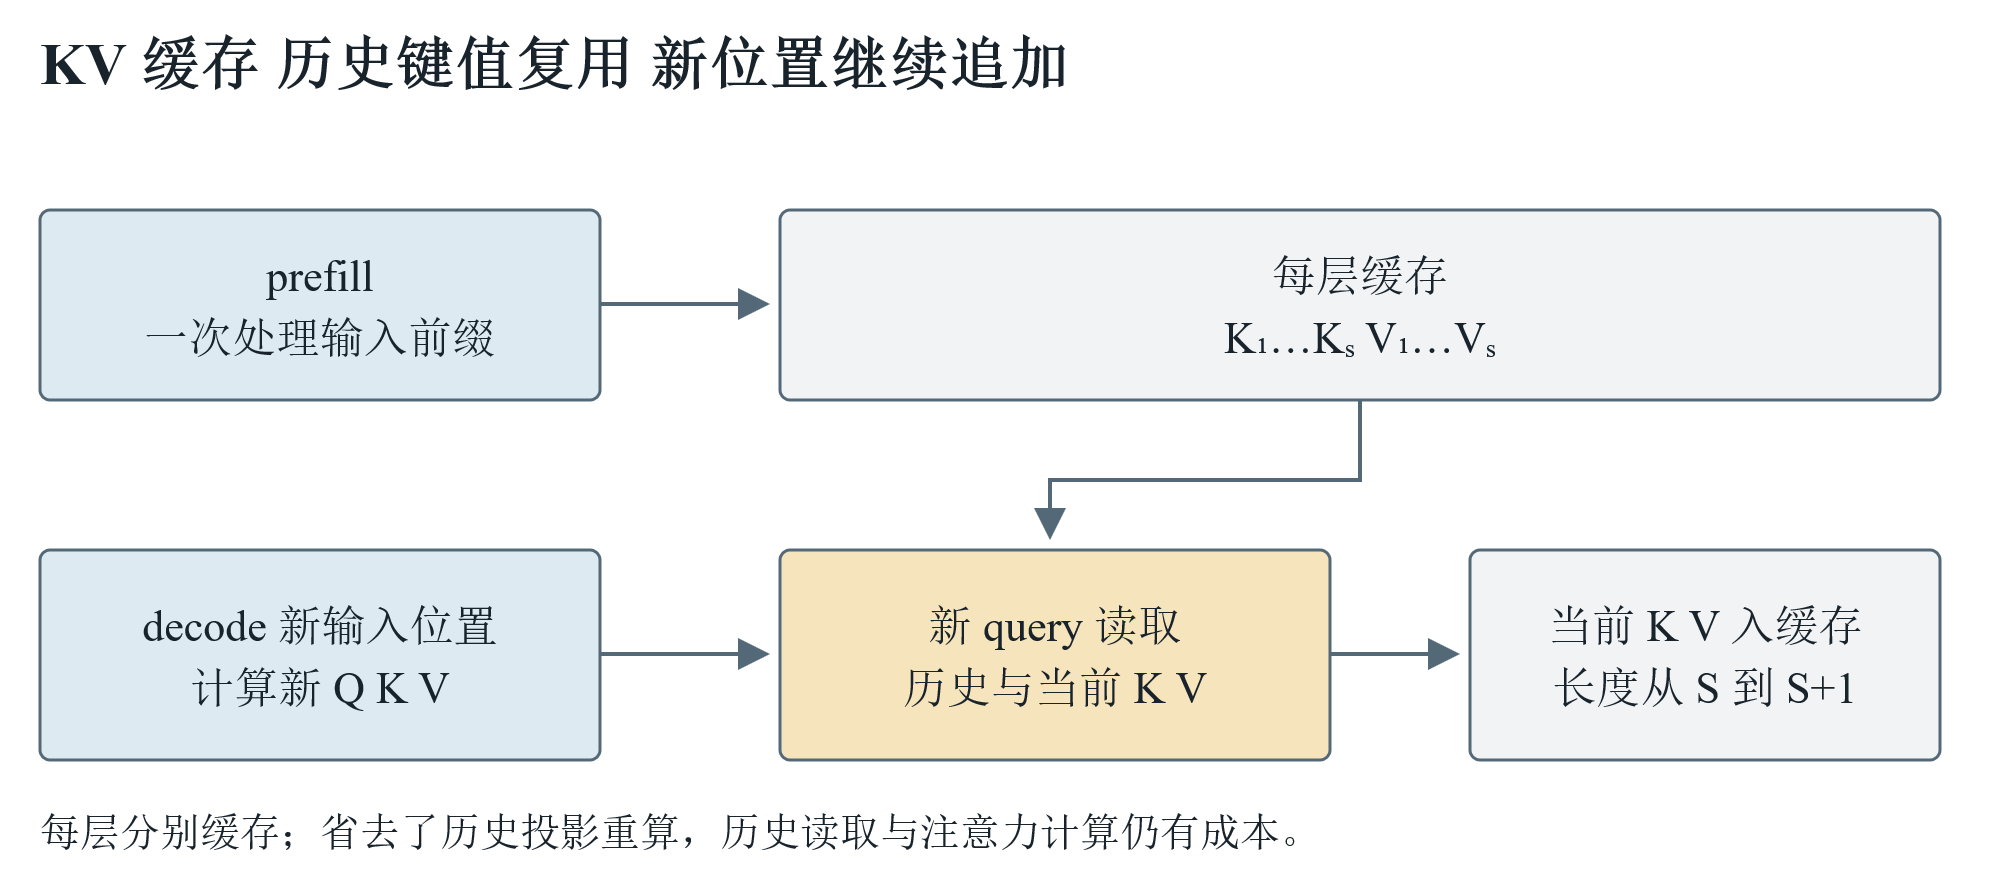
\includegraphics[width=\linewidth]{assets/media/image18.png}
    \caption{从 prefill 到 decode 的键值复用。每一层分别保存已处理位置的键和值；当前位置的查询读取这些缓存，计算注意力输出。}
    \label{fig:KV缓存复用}
\end{figure}

对一个简化的稠密注意力模型，单序列缓存占用可按两份张量、层数、KV 头数、头维度、序列长度与每元素字节数相乘估算。分组查询注意力（Grouped-Query Attention，GQA）让多个查询头共享一组 K、V，因此缓存容量由实际的 KV 头数决定。 用 M 表示字节占用，L 表示层数、H 的下标 KV 表示 KV 头数、d 表示头维度、S 表示缓存长度、b 表示每元素字节数，估算式为：
\[M_{KV} \approx 2\, L\, H_{KV}\, d\, S\, b\]

系数 2 对应 key 与 value 两份缓存。多个会话并发时，总缓存占用可以按各个会话的序列长度分别计算后求和。

例如 32 层、8 个 KV 头、每头 128 维、4096 个 token、每元素 2 字节，单序列 KV 约为 512 MiB。MiB 是二进制兆字节（mebibyte），1 MiB 等于 1,048,576 字节。完整的显存预算由模型权重、KV 缓存、计算临时缓冲和分配管理开销共同组成。缓存量化通过降低每元素字节数减少占用，滑动窗口通过限制保留的历史范围控制缓存长度。容量规划可以先按各会话长度估算 KV 缓存，再加上权重与运行时开销，确定可支持的并发规模。

FlashAttention 通过更好的计算与存储访问方式降低注意力的内存开销；PagedAttention 一类方案改善服务时的缓存管理。FlashAttention 侧重注意力计算中的数据读写与中间结果组织，PagedAttention 侧重多个请求的缓存分配与复用。评估服务性能时，首 token 延迟反映开始响应的等待时间，每秒生成 token 数反映输出速度，并发吞吐反映服务总处理能力，峰值显存决定运行容量。

部署还涉及权重量化、批处理和推测解码等方法。我们先了解它们各自在压缩权重、摊薄计算或减少主模型串行调用中的作用，再按实际瓶颈验证。量化后的评估包括关键任务准确率、对话模板兼容性、生成速度和显存占用，用来选择适合部署目标的精度与性能配置。

长推理轨迹会同时增加训练时的轨迹采样成本，以及服务时的解码步数、缓存长度与响应延迟。推理预算可以按任务难度分配：复杂任务保留更多求解步骤，简单任务尽早给出答案。模型选择、推理预算与服务配置共同决定任务质量、响应时间和单次请求成本。

\textbf{本节相关资料}
\begin{enumerate}
    \item Dao 等，2022，\href{https://arxiv.org/abs/2205.14135}{FlashAttention Fast and Memory-Efficient Exact Attention with IO-Awareness} 。阅读重点：计算复杂度与存储访问成本为什么要分别考虑。
    \item Ainslie 等，2023，\href{https://arxiv.org/abs/2305.13245}{GQA Training Generalized Multi-Query Transformer Models from Multi-Head Checkpoints} 。阅读重点：KV 头共享怎样影响缓存。
    \item Kwon 等，2023，\href{https://arxiv.org/abs/2309.06180}{Efficient Memory Management for Large Language Model Serving with PagedAttention} 。阅读重点：多请求场景下的缓存组织。
\end{enumerate}

\section{线性注意力 资源受限时怎样保留长程信息}\label{线性注意力}

上一节讨论的 KV 缓存保存历史位置的键和值。上下文越长，需要保存和读取的历史数据就越多。对于显存有限的设备、大量并发会话和持续生成的长任务，历史信息的存储与访问成为推理成本的重要来源。线性注意力（linear attention）通过改变历史信息的组织方式降低这部分开销，正成为资源受限条件下大模型架构的新兴研究与应用方向。

\textbf{从逐个读取历史到维护状态}~标准因果注意力在生成第 $t$ 个 token 时，让当前位置的查询与前 $t$ 个位置的键比较，再对相应的值加权求和。把长度为 $N$ 的整段序列处理完，需要计算的查询与键的配对数量按 $N^2$ 增长。线性注意力则把历史键值逐步汇总到一个状态中，新 token 到来时更新状态，再用当前查询读取状态。它像一份随阅读持续更新的工作笔记：已经读过的内容进入笔记，接下来的问题通过笔记取出相关信息。

以一种基础的核特征线性注意力为例，可以把因果计算写成：
\[
S_t=S_{t-1}+\varphi(k_t)v_t^{\mathsf T},\qquad
z_t=z_{t-1}+\varphi(k_t),\qquad
 o_t=\frac{S_t^{\mathsf T}\varphi(q_t)}{z_t^{\mathsf T}\varphi(q_t)}.
\]
这里，$t$ 是序列位置；$q_t$、$k_t$、$v_t$ 分别是该位置的查询、键和值列向量；$\varphi$ 是把查询和键映射为非负特征向量的函数。$S_t$ 是汇总到位置 $t$ 的键值状态矩阵，$z_t$ 是用于归一化的键特征累加向量，初始状态 $S_0$、$z_0$ 均为零。$\varphi(k_t)v_t^{\mathsf T}$ 是外积，把当前键与值的关联写入状态；上标 $\mathsf T$ 表示转置。$o_t$ 是读取状态后得到的输出向量，分母用于归一化，实际计算可加入一个很小的正数保持数值稳定。

当特征维度和值向量维度固定时，每次状态更新与读取的计算量不随历史长度增长，处理整段序列的注意力计算量便随 $N$ 线性增长；``线性''指的就是对序列长度的这种依赖关系。递推生成时，线性注意力层保存固定形状的状态，用状态更新替代不断追加历史键值。这个变化直接减少了长序列解码时的历史缓存与读取需求。

\textbf{从基础状态累加到现代混合架构}~状态相当于把历史压缩进有限容量的记忆。现代方法进一步学习哪些内容应保留、遗忘或改写，例如通过门控调节记忆保留比例，通过增量更新修正已有的键值关联。混合架构把线性注意力层与完整注意力层组合：线性层高效更新历史状态，完整注意力层按位置访问历史内容，层的配比决定了记忆方式与资源开销。

Kimi 等主流大模型团队已经把线性注意力用于实际模型架构。月之暗面在 2025 年发布的 Kimi Linear 采用 Kimi Delta Attention（KDA）与多头潜在注意力（Multi-Head Latent Attention，MLA）混合的设计，并公开了模型权重和推理实现。KDA 通过细粒度门控管理有限状态记忆，MLA 层保留完整注意力的信息访问方式。Kimi Linear 展示了线性注意力从基础算法进入大规模预训练与推理部署的实践路径。

资源受限场景推动这条路线继续发展：固定形状的状态降低长会话的缓存增长，门控与记忆更新提高状态的信息利用率，混合层设计协调精确检索与持续计算。对于需要处理长文档、维护多轮工具轨迹或同时服务大量用户的模型，历史信息怎样进入记忆、记忆怎样被读取，已经成为模型架构设计的核心问题。

\textbf{本节相关资料}
\begin{enumerate}
    \item Katharopoulos 等，2020，\href{https://arxiv.org/abs/2006.16236}{Transformers are RNNs: Fast Autoregressive Transformers with Linear Attention}。阅读重点：核特征形式怎样把注意力改写成可递推计算。
    \item Kimi Team 等，2025，\href{https://arxiv.org/abs/2510.26692}{Kimi Linear: An Expressive, Efficient Attention Architecture}。阅读重点：KDA 的状态更新与门控，以及 KDA、MLA 混合架构的资源效率。
\end{enumerate}


\chapter{检索增强生成（RAG）}\label{检索增强生成}

\section{检索增强生成 RAG 让回答获得外部依据}\label{检索增强生成 RAG 让回答获得外部依据}

小助能解方程，却不知道``本周作业最晚何时提交''。提交时间由课程最新通知决定，相关材料保存在课程资料库中。我们让小助先检索通知，再根据通知中的日期与适用条件回答。

检索增强生成（Retrieval-Augmented Generation，RAG）已经成为大模型应用中的基础技术，广泛用于企业知识库问答、客服助手、产品文档查询和内部资料检索。它把信息检索与语言生成连接起来：检索系统负责找到当前问题需要的材料，语言模型负责阅读材料并组织回答。资料库可以独立维护，新通知或新文档进入检索范围后，模型就能在回答时使用这些内容。

RAG 的核心是把检索到的外部材料纳入生成条件。模型利用参数中学到的语言与任务能力理解问题，以可更新资料库中的材料作为回答依据。回答质量取决于资料是否准确、检索是否完整，以及模型能否正确解释和引用证据。保存检索结果与来源位置，可以沿这些环节检查答案的形成过程。

\textbf{先区分建库与回答两个阶段}~建库阶段把 PDF、网页或办公文档解析成文本，保留标题、表格和来源信息，再切分、编码并建立索引。扫描版文件可以先通过光学字符识别（Optical Character Recognition，OCR）取得文字。回答阶段接收用户问题，检索相关片段，将片段与问题一起送入模型。常见的工程流程可以复用已有嵌入模型与生成模型，更新资料主要涉及文档处理和索引维护，生成模型的参数保持固定。

我们先把课程文件切成段落。按固定长度切分容易把``允许迟交''和``超过多久不计分''分到两个片段，读者需要结合两个片段才能得到完整规则。我们结合标题、段落、表格与适度重叠，让每个文本片段（chunk）保有必要上下文，同时保存文档名、版本、页码或段落编号。重叠过多会增加重复检索，切得太大又会把相关句子淹没在噪声里，因此要用查询与证据覆盖率选择。

接着，我们用嵌入模型把每个片段编码成向量，并把向量、原文与来源标识关联保存。索引是用于快速找到候选片段的数据结构，可以由向量数据库、搜索引擎或本地检索程序提供。收到问题后，同一个嵌入模型把问题编码成查询向量，检索程序按向量相似度选出候选片段，这个步骤称为召回。常用的余弦相似度衡量两个向量方向的接近程度，得分用于排序候选的相关性。资料量较大时，近似最近邻（Approximate Nearest Neighbor，ANN）索引用较少的比较找到接近查询向量的候选，提高检索速度。若课程名称或作业编号很关键，可以同时做最佳匹配 25（Best Matching 25，BM25）等词法检索，再融合结果。向量检索利用语义联系匹配不同措辞，词法检索利用关键词匹配课程名称、作业编号等精确信息。混合检索将两类候选合并，再通过重排选出与问题最相关的材料。

召回后，我们可用交叉编码器（cross-encoder）重排。双塔嵌入先把查询和文档分别编码，便于大规模比较；cross-encoder 让查询与候选一起进入模型，进行更细的相关性判断，代价也更高。我们因此只用它处理有限候选。

最后，我们把少量证据与问题一起交给小助，要求回答中标明依据，证据不足时说明缺口。检索程序按用户访问权限筛选可用文档，生成器把检索片段作为待分析的资料处理。工具权限与任务规则由应用层管理，文档中的操作性文字按资料内容解释。

\textbf{把一次问答完整走通}~假设课程资料中有三个片段：片段 A 说明作业一的提交时间，片段 B 说明作业二截止于周五 18:00，片段 C 说明迟交扣分规则。用户问``作业二什么时候交？''，系统先检索一批候选，再把最相关的片段 B 放到前面。工程中常把返回得分最高的 $k$ 个候选称为 top-$k$，其中 $k$ 是候选数量；例如先召回 20 个片段，再重排选出 3 个组成模型输入。召回数量决定初选范围，最终选入数量则影响阅读成本与证据覆盖。

交给生成器的输入可以组织成下面的形式：
\begin{quote}
任务：依据课程资料回答问题，给出资料编号。\\
资料 [1]：《课程通知》第 2 节，作业二于周五 18:00 截止。\\
问题：作业二什么时候交？
\end{quote}
模型据此回答``作业二于周五 18:00 截止，依据《课程通知》第 2 节 [1]''。检索阶段选出的文字通过上下文进入这次前向计算，来源标识则把答案与原文位置连接起来。若用户继续询问迟交规则，系统可围绕新问题检索片段 C，再生成对应解释。

资料维护也沿着同一条链进行。课程通知更新时，为新版本重新切分和编码，并更新索引中的对应记录；旧版本可以归档，并用生效日期与版本字段区分。查询时先按课程、年份和访问权限筛选，再在符合条件的资料中检索，回答便能对应到当前适用的通知。

图 \ref{fig:RAG证据链} 将离线建库与在线回答分成两条路径。离线索引保存可检索的表示与来源，在线过程才根据这次问题选择证据。

\begin{figure}[t]
    \centering
    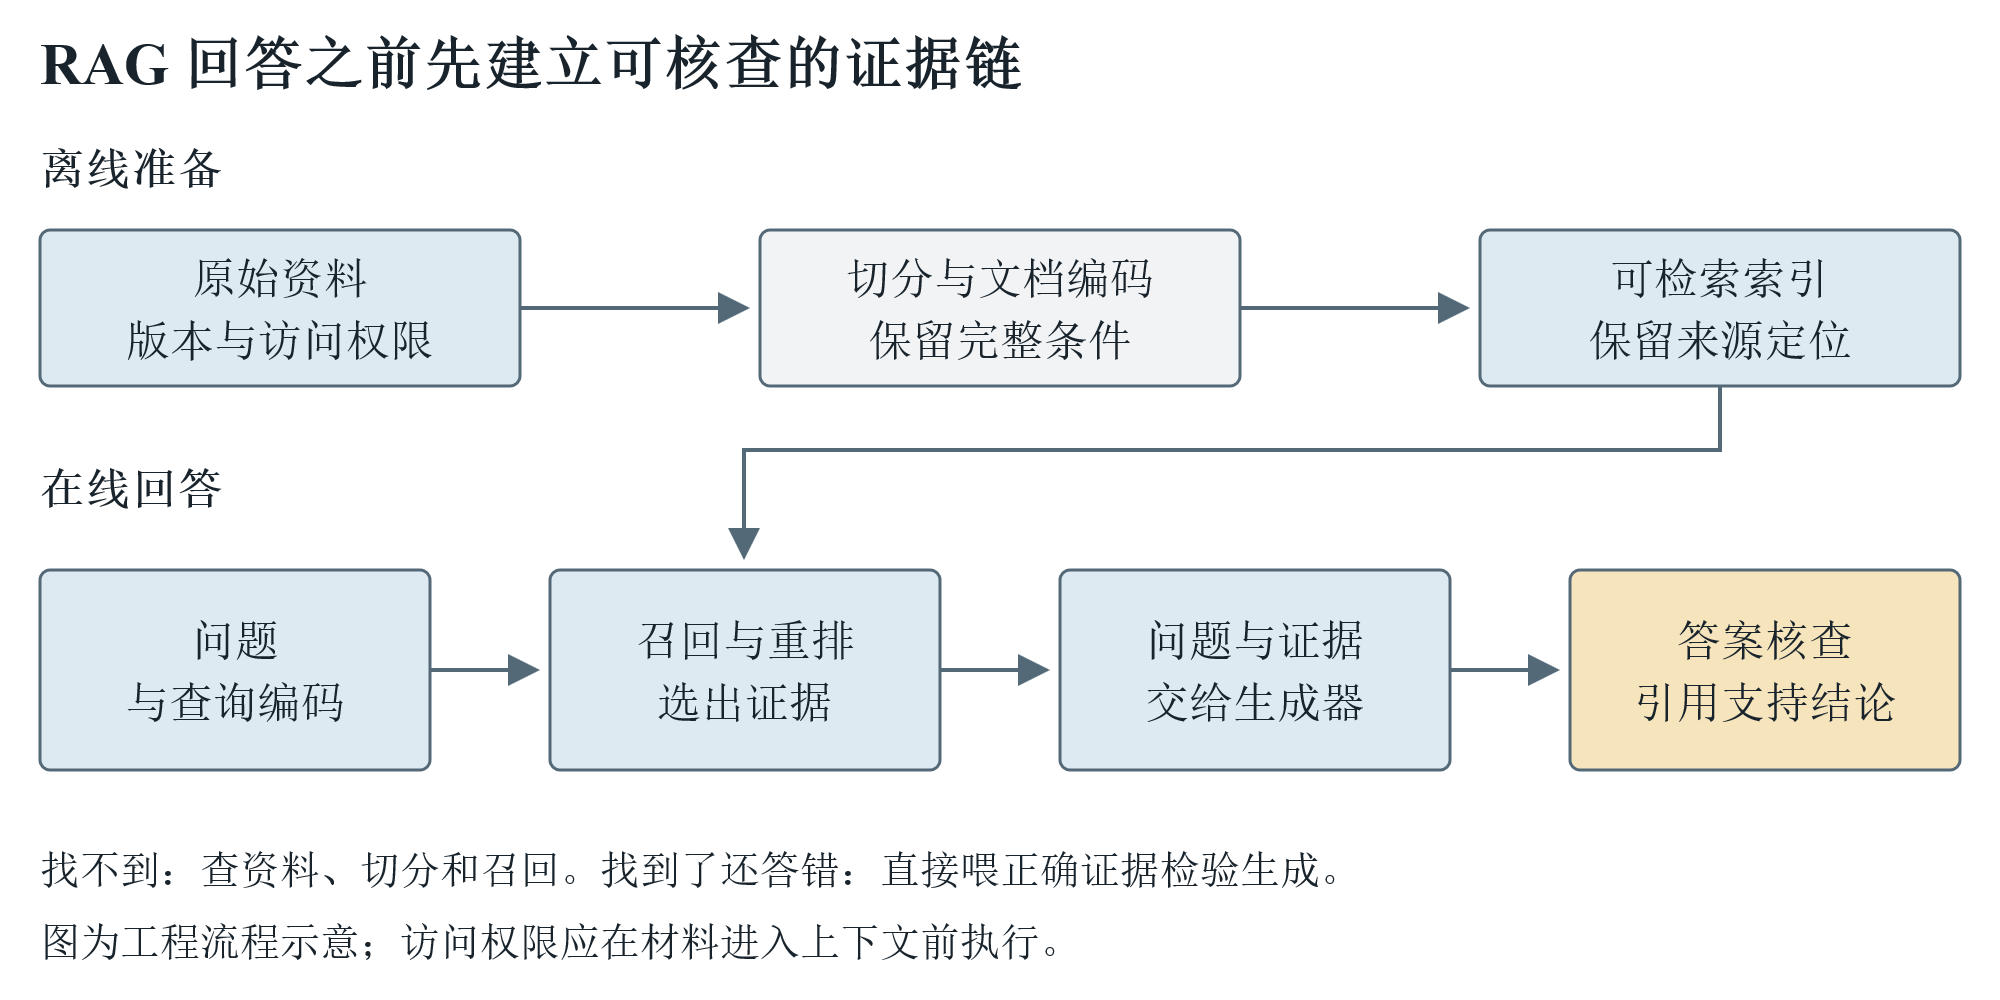
\includegraphics[width=\linewidth]{assets/media/image20.png}
    \caption{RAG 的工程证据链。资料版本、访问权限和来源定位贯穿流程；正确证据交给生成器后是否仍答错，是下一节诊断的关键分叉。}
    \label{fig:RAG证据链}
\end{figure}

我们完成的是一条可逐段检查的证据链：正确材料存在吗，切分保留了吗，召回找到了吗，重排留下了吗，生成忠实使用了吗？下一节就沿这条链定位失败。

\textbf{本节相关资料}
\begin{enumerate}
    \item Lewis 等，2020，\href{https://arxiv.org/abs/2005.11401}{Retrieval-Augmented Generation for Knowledge-Intensive NLP Tasks} 。阅读重点：参数化知识与外部检索如何结合。原论文联合建模检索与生成，工程实践也常采用分别训练的检索器与生成器组成管线。
    \item \href{https://cloud.google.com/use-cases/retrieval-augmented-generation}{Google Cloud：What is Retrieval-Augmented Generation (RAG)?}。阅读重点：RAG 的基本流程与知识库问答等应用场景。
    \item Nogueira 与 Cho，2019，\href{https://arxiv.org/abs/1901.04085}{Passage Re-ranking with BERT} 。阅读重点：联合编码查询与文档为什么适合重排。
\end{enumerate}

\section{RAG 诊断 沿证据链定位失败}\label{RAG 诊断 沿证据链定位失败}

我们问``作业允许迟交几天''，小助引用了一段相关资料，却答错限制条件。只看最终答案，我们不知道该换嵌入模型、扩大上下文，还是重训生成器。我们于是为每个失败保存完整过程：查询、候选、分数、选入上下文的证据和最终回答。

第一步做 oracle context 实验：直接把人工确认的正确证据交给生成器。如果这时仍答错，优先检查阅读、提示、冲突处理或任务能力；如果这时答对，问题更可能在前面的检索与组织。正确证据条件下的回答结果，为后续选择检索侧或生成侧的改进提供依据。

\textbf{用小型评测集建立基线}~可以先收集一组真实问题，为每个问题标出正确答案和支持答案的资料位置。检索阶段检查正确证据是否进入候选，生成阶段检查答案是否正确、引用是否支持结论。若一个问题有 4 个标注为相关的片段，前 $k$ 个检索结果找到了其中 3 个，该问题的召回率 Recall@$k$ 就是 $3/4=75\%$；如果前 $k$ 个结果中有 3 个相关片段，精确率 Precision@$k$ 就是 $3/k$。这里 $k$ 表示检查的检索结果数量。多个问题分别计算后取平均，可以比较切分、检索与重排配置。

对于需要合并多份材料的问题，还要检查关键证据是否收齐。例如，判断某次迟交是否扣分，需要同时取得截止时间与迟交规则。生成侧则逐项核对日期、数值、条件和来源，并记录响应延迟与输入 token 数。证据覆盖、答案质量与运行成本一起构成 RAG 入门系统的评估记录。

随后逐段检查。正确证据不在资料库，是信息缺失；原文有而 chunk 不完整，是切分问题；穷举相似度能找到、ANN 找不到，是索引召回问题；召回中有、重排后丢了，是重排问题；上下文中有、答案仍歪曲，是生成使用问题。每次只替换一个组件，并比较相同查询上的证据与答案变化，就能判断改动影响了哪个环节。

若查询太短或术语错位，可以尝试查询改写。假设文档嵌入（Hypothetical Document Embeddings，HyDE）先生成一个假设性文档，再用它做检索桥梁；假设文档提供与目标材料接近的语义表达，作为检索查询的中间表示；最终回答引用实际检索到的原始资料。

若用户问的是整套课程材料的共同主题，系统需要汇总跨文档信息。图检索增强生成（Graph Retrieval-Augmented Generation，GraphRAG）通过实体、关系或社区摘要组织材料，支持全局主题归纳；建库流程相应增加关系抽取、建图和摘要更新。对于需要逐步补全证据的问题，智能体式检索增强生成（agentic RAG）根据当前结果识别信息缺口，再发起下一次检索。第七章的工具调用循环在这里具体表现为查询、阅读结果、补充查询与组织答案。

对于规模可控、需要跨段联系的资料，可以直接把完整材料放入长上下文，建立综合阅读基线。评估时检查不同证据位置下的回答质量、跨段信息整合能力，以及输入长度带来的延迟和成本。对于持续更新的大型资料库，先检索再阅读可以缩小每次输入的材料范围；检索与长上下文结合，则能把多份相关文档交给模型联合分析。下表按信息获取与行为调整的需求，列出可比较的方案。

\begin{longtable}[]{@{}
  >{\raggedright\arraybackslash}p{(\linewidth - 4\tabcolsep) * \real{0.2985}}
  >{\raggedright\arraybackslash}p{(\linewidth - 4\tabcolsep) * \real{0.2985}}
  >{\raggedright\arraybackslash}p{(\linewidth - 4\tabcolsep) * \real{0.4030}}@{}}
\toprule\noalign{}
\begin{minipage}[b]{\linewidth}\raggedright
\textbf{需求}
\end{minipage} & \begin{minipage}[b]{\linewidth}\raggedright
\textbf{优先建立的基线}
\end{minipage} & \begin{minipage}[b]{\linewidth}\raggedright
\textbf{关键验证}
\end{minipage} \\
\midrule\noalign{}
\endhead
\bottomrule\noalign{}
\endlastfoot
少量完整资料的综合阅读 & 长上下文直接阅读 & 位置变化与跨段整合 \\
经常更新的大型资料库 & RAG & 召回和引用支持度 \\
稳定改变输出行为或格式 & SFT & 新行为与旧能力回归 \\
新知识与新行为同时需要 & 检索与训练组合 & 分别测信息获取和行为执行 \\
\end{longtable}

\textbf{本节相关资料}
\begin{enumerate}
    \item Gao 等，2022，\href{https://arxiv.org/abs/2212.10496}{Precise Zero-Shot Dense Retrieval without Relevance Labels}，HyDE 。阅读重点：假设文档怎样构造检索表示，以及原始资料怎样支持最终回答。
    \item Edge 等，2024，\href{https://arxiv.org/abs/2404.16130}{From Local to Global A Graph RAG Approach to Query-Focused Summarization} 。阅读重点：全局问题与局部段落检索的差别。
    \item Liu 等，2023，\href{https://arxiv.org/abs/2307.03172}{Lost in the Middle How Language Models Use Long Contexts} 。阅读重点：证据位置与输入长度怎样影响模型的信息利用。
\end{enumerate}


\chapter{可解释性入门}\label{可解释性入门}

大模型能够生成复杂回答，研究者也希望理解这些行为对应的内部计算。可解释性研究由此连接两个问题：模型的表示中包含什么信息，这些信息怎样参与预测。在学术研究中，相关方法从输入特征归因、表示探针和注意力分析，逐步扩展到激活干预、计算回路发现与稀疏特征分解。研究对象也从小模型上的可控任务，扩展到大语言模型中的知识提取、关系判断与多步生成。

工业界对这条路线同时存在投入与质疑。Anthropic 等企业研究团队持续研究特征提取与计算路径追踪，希望把内部分析用于模型诊断、行为监测和定向调整。面向产品落地的质疑则集中在实际收益：分析一个行为需要多少计算与人工，发现的特征能否在新输入和模型版本上复现，内部干预相对于直接评测、数据改进和重新训练带来多少增益。Google Research 的相关工作也将应用目标和评估指标的标准化，列为判断可解释性方法实用价值的重要问题。

可解释性的潜力在于把输出差异追踪到具体表示与计算路径，为错误定位、训练诊断和模型控制提供更细的实验依据。当前的主要局限是分析覆盖范围、解释粒度与研究成本：局部回路通常围绕特定任务建立，稀疏特征的描述需要样本与干预验证，大模型的激活采集和分析也需要额外资源。因而，本章从可重复的小实验入手，依次介绍信息读出、状态替换和特征分解，让读者掌握提出机制假设并检验它的基本方法。

\textbf{引入阅读}
\begin{enumerate}
    \item Anthropic，2025，\href{https://www.anthropic.com/research/tracing-thoughts-language-model}{Tracing the thoughts of a large language model}。阅读重点：计算路径追踪的研究进展、应用动机与分析成本。
    \item \href{https://research.google/pubs/towards-unifying-interpretability-and-control-evaluation-via-intervention/}{Towards unifying interpretability and control: Evaluation via intervention}。阅读重点：以可测量的干预效果评估可解释性方法的实用价值。
\end{enumerate}

\section{可解释性的证据~看到了什么与证明了什么}\label{可解释性的证据 看到了什么与证明了什么}

前面的训练诊断让我们发现：小助的回答变短，可能只是行为倾向变化；一个词生成不出来，也可能涉及输出端偏移。我们已经能通过输入与输出比较排除一些解释，但还会追问：模型内部到底利用了哪些信息，又通过什么计算形成这次答案？这就是可解释性（interpretability）要帮助我们研究的问题。

我们先区分两个尺度。行为分析改变提示、数据或工具，观察系统如何反应；机制可解释性（mechanistic interpretability）进一步研究参数、激活与计算路径，尝试用可检验的机制解释特定行为。解释的对象可以是一道题、一个注意力头，也可以是跨一批输入反复出现的计算模式。实验开始时写明模型、输入类型与目标行为，后续观察和干预围绕这些对象展开。

最容易上手的是注意力热图。假设小助生成``她''时，一个头对某个人名分配较大权重，这是一条有价值的观察。权重描述该注意力头混合各位置值向量的比例。分析这个头对答案的作用，还需要结合值向量的内容、输出投影、残差流和后续层的计算。热图提供候选位置，针对这些位置的干预实验进一步检验它们对输出的影响。

小助还可以自己解释：``我先根据代词找到人名，再回答。''这段文字描述了模型给出的解题过程，可以帮助读者检查步骤、提出机制假设。研究者再通过改变人名、代词和中间激活，比较回答变化，检验文字解释与实际计算之间的对应关系。

我们把证据分成三层：观察到某个激活与行为相关；从表示中读出某类信息；干预某处计算后，目标行为按预测改变。相关性分析用于发现候选，读出实验用于检查表示中的信息，干预实验用于检验计算对行为的影响。接下来依次介绍读出与受控干预。

\textbf{本节相关资料}
\begin{enumerate}
    \item Jain 与 Wallace，2019，\href{https://arxiv.org/abs/1902.10186}{Attention is not Explanation} 。阅读重点：注意力权重、预测结果与干预效果之间的关系。
    \item Turpin 等，2023，\href{https://arxiv.org/abs/2305.04388}{Language Models Don't Always Say What They Think Unfaithful Explanations in Chain-of-Thought Prompting} 。阅读重点：解释文本如何遗漏实际影响回答的因素。
\end{enumerate}

\section{线性探针 表示中能读出什么}\label{线性探针 表示中能读出什么}

我们怀疑小助在某一层已经表示了``谁把物品给了谁''，但最后没有选对人名。怎样判断信息是在中途丢失，还是存在却没有被后续计算有效利用？一种入门办法是在线性探针（linear probe）上做实验：冻结模型，只训练一个很小的读出器。

\textbf{先定义标签：谁是物品接收者}~标签由研究者根据任务定义并标注。这里把句子中第一次出现的两个人名依次记为人物 1、人物 2，并规定：接收者是人物 1 时，标签 $c=0$；接收者是人物 2 时，标签 $c=1$。例如：
\begin{itemize}
    \item ``小明把书交给了小红。''人物 1 是小明，人物 2 是小红，接收者是小红，因此标签为 1。
    \item ``小明从小红那里收到了书。''人物顺序相同，接收者是小明，因此标签为 0。
    \item ``小红把笔递给了小明。''人物 1 是小红，人物 2 是小明，接收者是小明，因此标签为 1。
    \item ``小红从小明那里接过了笔。''人物顺序相同，接收者是小红，因此标签为 0。
\end{itemize}
这个标签把句子的人物关系变成了一个二分类任务。人物编号按每个句子的出现顺序确定，类别 0 和类别 1 分别对应第一位和第二位人物。更换姓名和物品后，标注规则保持一致。

\textbf{输入探针的是什么}~把完整句子送入冻结的语言模型，取第 $l$ 层、句末最后一个有效 token 位置的隐藏向量 $h$。这里 $l$ 是选定的层编号，$h$ 是一个 $d$ 维向量，$d$ 是模型隐藏维度。因果语言模型在句末位置已经能够读取此前整句，因此这个位置适合用来检查接收者信息。每个句子产生一对训练数据 $(h,c)$：$h$ 来自语言模型，$c$ 来自事先确定的关系标注。只把句子送入语言模型，标签用于探针的损失计算。

\textbf{探针本身需要训练}~线性探针是在隐藏向量上训练的分类器。为每个句子提取 $h$ 后，随机初始化分类器的权重 $W$ 和偏置 $b$，再用带标签的数据学习如何读取这些向量。类别概率写为：
\[
P_\phi(c\mid h)=\operatorname{softmax}(Wh+b)_c.
\]
这里，$W\in\mathbb R^{2\times d}$ 把 $d$ 维隐藏向量映射为两个类别的分数，$b\in\mathbb R^2$ 为两个类别分别提供偏置；$\phi=\{W,b\}$ 表示探针的全部可训练参数。softmax 把两个分数归一化为概率，下标 $c$ 表示取真实标签对应的概率。例如，标签为 1 的句子需要读取类别 1 的预测概率。

假设训练集有 $N$ 个样本，探针使用交叉熵损失：
\[
L_{\mathrm{probe}}(\phi)
=-\frac{1}{N}\sum_{i=1}^{N}\log P_\phi(c_i\mid h_i).
\]
$N$ 是训练样本数，$i$ 是样本编号，$h_i$ 是第 $i$ 个句子的隐藏向量，$c_i$ 是对应的真实标签，$\log$ 是自然对数。优化器通过梯度下降更新 $W$ 和 $b$，提高真实标签的预测概率。若某个标签为 1 的样本最初只得到 0.4 的预测概率，其损失约为 $-\ln0.4=0.916$；训练后该概率提高到 0.8，损失就降为约 0.223。整个过程中，原语言模型的参数保持冻结，隐藏向量可以预先提取并保存，之后单独训练探针。

训练完成后，在未用于训练的句子上提取同样位置的隐藏向量，由探针预测接收者是人物 1 还是人物 2，再与真实标签比较，计算准确率。分别对不同层的隐藏向量训练独立探针，就能比较接收者关系在各层表示中的可读出程度。

如果探针在独立数据上表现很好，可以说明这些表示中存在可由该读出器利用的信息。探针负责检验信息的可读出性，原模型怎样利用这些信息则由后续计算决定。研究者可以根据探针结果选择候选层，再通过激活修补观察相应信息对原任务输出的影响。

实验设置三类控制：按句型和实体划分训练与测试数据，检查对新句型和新实体的泛化；与词频、位置等简单基线比较，识别表面统计线索；训练打乱标签的探针，估计读出器记忆任意标签的能力。我们尽量保持探针简单，并报告正则化与数据量。探针越复杂，越难区分``从原表示读取''与``读出器自己学会了任务''。

不同层的探针准确率展示指定标签在各层表示中的可读出程度。实验报告同时记录标签定义、读取位置与数据划分，便于比较准确率曲线。准确率较高或发生明显变化的层，可以作为因果干预的候选位置。

\textbf{本节相关资料}
\begin{enumerate}
    \item Alain 与 Bengio，2016，\href{https://arxiv.org/abs/1610.01644}{Understanding intermediate layers using linear classifier probes} 。阅读重点：冻结模型、训练读出器的实验结构，以及表示可读出性与原任务行为的区别。
    \item Wang 等，2022，\href{https://arxiv.org/abs/2211.00593}{Interpretability in the Wild A Circuit for Indirect Object Identification in GPT-2 small} 。阅读重点：为什么机制分析需要把表示观察与更直接的行为干预结合。
\end{enumerate}

\section{激活修补 用干预检验计算路径}\label{激活修补 用干预检验计算路径}

我们准备一个比课程问答更容易控制的小任务。提示是``When Alice and Bob went to the library, Alice gave the book to''，模型应更偏向续写 Bob。把后半句的 Alice 换成 Bob，预期答案随之换成 Alice。这类间接宾语识别（Indirect Object Identification，IOI）任务具有明确的候选答案和可控制的人物关系，适合作为入门实验。

首先，我们确认所选模型在这批原始提示上确实表现出目标行为，并检查候选名字在 tokenizer 中是否各占一个 token。对于多 token 候选，比较完整续写的对数概率；对于单 token 候选，可以直接比较末尾位置的输出分数。这里先使用单 token 候选，方便定义测量。

我们把末尾位置对 Bob 和 Alice 的 logits 分别记为 z 的下标 Bob 与 Alice。用两个候选的分数差衡量模型的输出倾向：
\[\Delta z = z_{Bob} - z_{Alice}\]

Δz 越大，表示模型相对更偏向 Bob；Δz 可以取任意实数，正值偏向 Bob，负值偏向 Alice。先记录原始输入与对照输入的基线分数差，再以两者的差异作为修补实验的比较基准。

接着做激活修补（activation patching）：缓存原始运行某层、某位置的激活；运行对照输入时，只把这一处替换为原始激活，其他计算保持对照运行的状态；然后观察 Δz 是否朝原始方向恢复。这是在固定参数下修改一次前向计算，和改写权重的模型编辑不同。

\textbf{具体替换哪一个向量}~选定第 $l$ 层输出的残差流作为修补对象，把位置 $p$ 的向量记为 $h_{l,p}$。残差流是注意力与前馈网络等组件的输出通过残差连接累加形成的表示。$l$ 表示层编号，$p$ 表示 token 位置；实验记录层输出这一具体读取点，使不同运行使用相同的定义。原始提示的对应向量记为 $h^{\mathrm{orig}}_{l,p}$，对照提示的对应向量记为 $h^{\mathrm{ctrl}}_{l,p}$。修补操作是
\[
h^{\mathrm{ctrl}}_{l,p}\leftarrow h^{\mathrm{orig}}_{l,p}.
\]
箭头表示赋值替换。原始输入在这里提供一份激活，对照输入提供被干预的运行；替换后，后续网络层基于修改后的状态重新计算。模型参数在整个过程中固定。

例如，选择前述两个提示末尾的 to 所在位置。先运行原始提示，保存指定层该位置的向量；再运行对照提示，在同一层、同一位置用保存的向量替换当前向量，继续算到输出端。计算机实现通常通过前向钩子（forward hook）读取和替换中间张量。由于后续状态依赖被替换的向量，修补影响会通过后续层传播到候选名字的分数。

\begin{figure}[t]
    \centering
    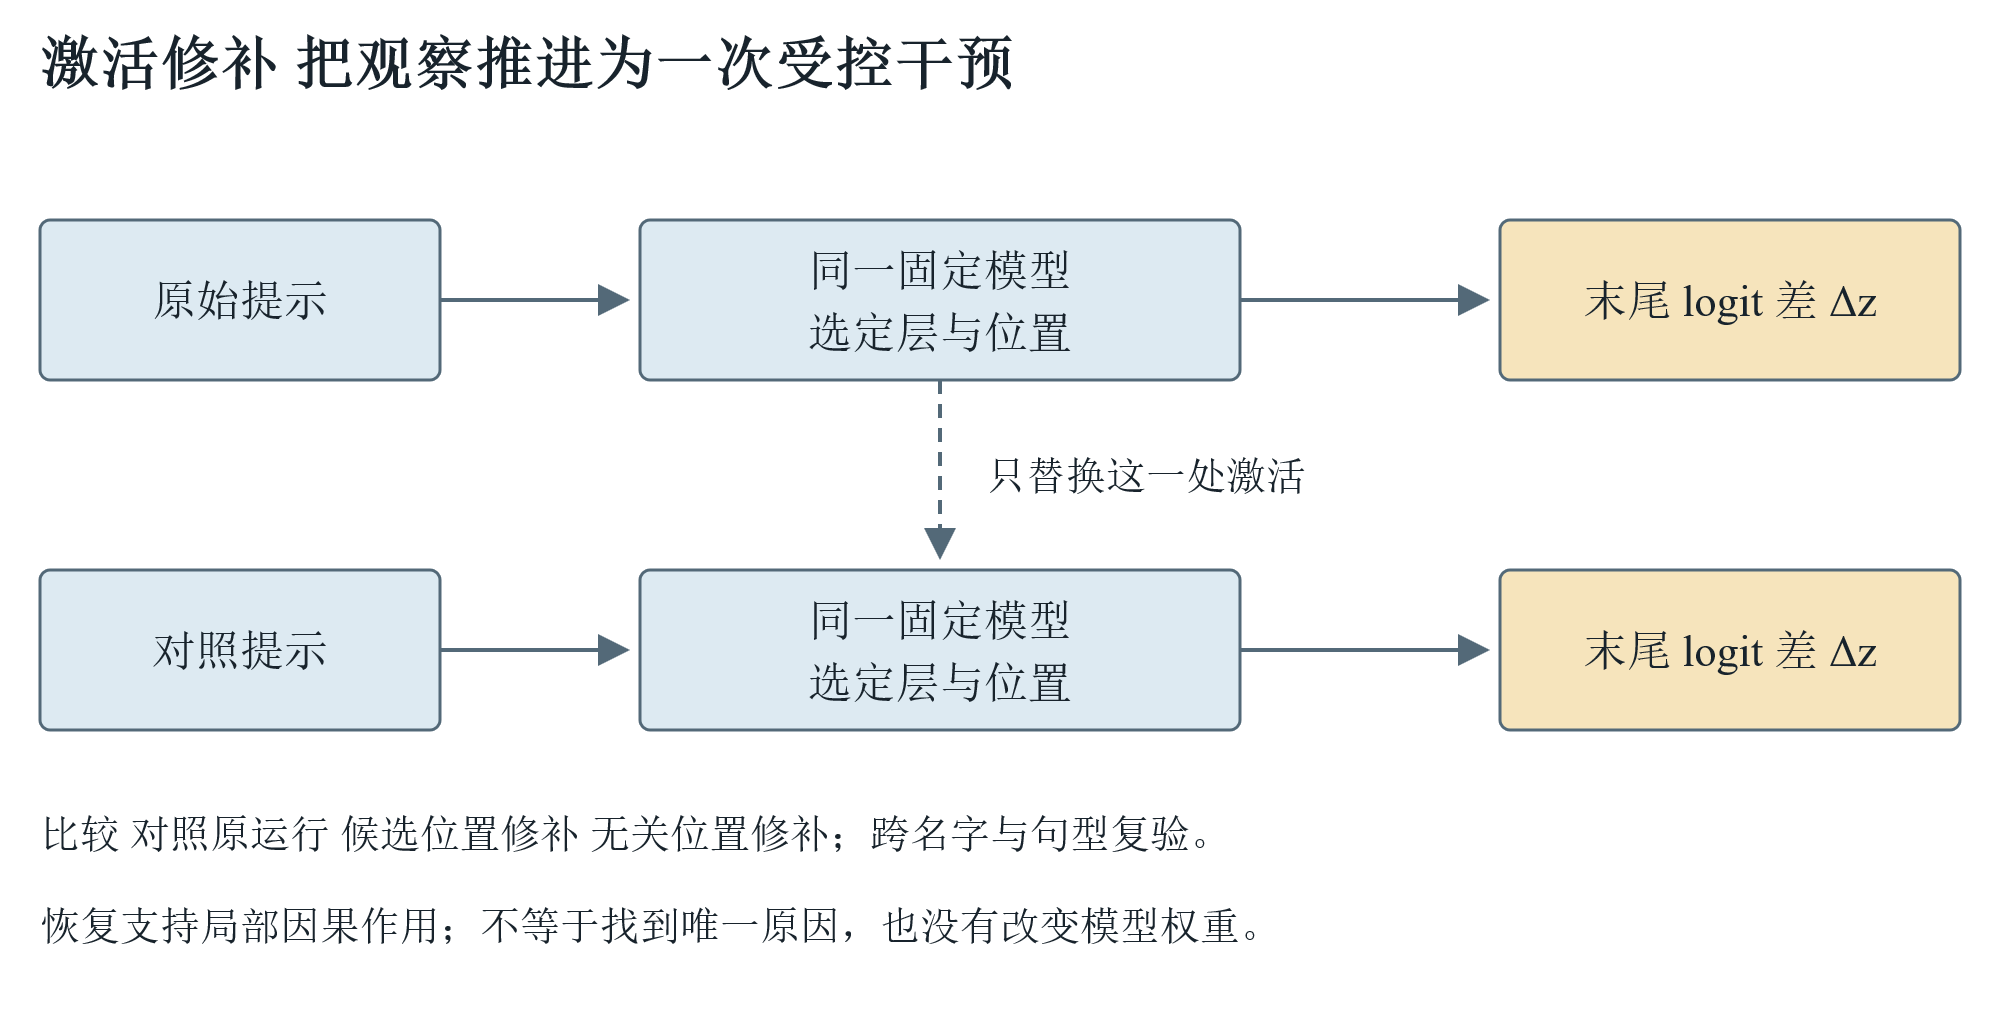
\includegraphics[width=\linewidth]{assets/media/image22.png}
    \caption{激活修补的受控实验。虚线表示将原始运行的指定激活替换到对照运行中；无关位置的修补提供负对照。}
    \label{fig:激活修补实验}
\end{figure}


\textbf{用三次运行计算恢复程度}~一次候选位置实验包含原始运行、对照运行和修补运行。假设三次运行的 Bob 与 Alice 分数差分别是 4、$-2$ 和 1。对照输入原本偏向 Alice，修补后转向 Bob。可以定义归一化恢复分数
\[
\rho=\frac{\Delta z_{\mathrm{patch}}-\Delta z_{\mathrm{ctrl}}}
{\Delta z_{\mathrm{orig}}-\Delta z_{\mathrm{ctrl}}}.
\]
$\Delta z_{\mathrm{orig}}$、$\Delta z_{\mathrm{ctrl}}$、$\Delta z_{\mathrm{patch}}$ 分别是原始、对照和修补运行的 logit 差，$\rho$ 表示修补填补了多少原始与对照之间的分数差距。上例中 $\rho=(1-(-2))/(4-(-2))=0.5$，即恢复了差距的 50\%。$\rho=0$ 表示与对照相同，$\rho=1$ 表示达到原始分数差；负值表示朝相反方向移动，大于 1 表示超过原始分数差。这个比值要求两条基线之间存在清晰差异，实验同时报告三次运行的原始分数，便于理解恢复幅度。

逐层、逐位置重复修补，可以画出恢复分数热图。比如某个位置在中间几层反复得到较高分数，就优先检查该位置相关的注意力头或前馈网络。随后在新句型上复验，并与无关位置修补、相同输入自修补比较，将候选范围缩小到具体计算组件。

图 \ref{fig:激活修补实验} 中，两次运行共享全部权重。竖向虚线只替换一个明确指定的中间状态；其后计算继续使用对照输入的其余状态。记录干预前后的 logit 差，可以量化修补对候选倾向的影响，并比较多个输入上的效果。

如果一个位置的修补稳定恢复了倾向，我们获得了``在这组输入和干预方式下，这处状态携带了影响输出的信息''的证据。接下来更换名字、句型与对照方式复验，并修补无关位置作负对照。源激活与目标位置按角色和位置对齐，使替换后的状态与当前计算保持可比较的语义条件。

我们再用消融（ablation）检查另一侧：移除、替换为均值或重采样某个组件的输出，行为是否受损？移除、均值替换和重采样分别改变组件输出的不同统计性质，实验记录具体操作并比较效果。对于多条路径共同完成的行为，可以组合消融多个组件，检验路径之间的补偿关系。把组件、连接和信息传递顺序组织起来，就形成可重复检验的计算回路（circuit）假设。

\textbf{本节相关资料}
\begin{enumerate}
    \item Wang 等，2022，\href{https://arxiv.org/abs/2211.00593}{Interpretability in the Wild A Circuit for Indirect Object Identification in GPT-2 small} 。阅读重点：怎样把一个可控行为分解成候选组件与计算路径。
    \item Zhang 与 Nanda，2023，\href{https://arxiv.org/abs/2309.16042}{Towards Best Practices of Activation Patching in Language Models Metrics and Methods} 。阅读重点：对照构造、度量和修补方式为什么会改变结论。
\end{enumerate}

\section{叠加表示与稀疏自编码器~一个神经元未必对应一个概念}\label{叠加表示与稀疏自编码器 一个神经元未必对应一个概念}

做完修补，我们查看一个候选神经元的高激活文本，发现它既回应课程说明，也回应某些代码片段。这些输入共享哪些特征，需要结合更多激活样本分析。模型中的特征可以沿多个神经元共同构成的方向表示，因此单个坐标上的激活会混合多种信息。

叠加表示（superposition）研究一种可能性：许多特征利用不完全正交的方向共享有限维度。当每次只出现少量相关特征时，这种共享可能仍有用。这种表示方式使同一个神经元参与多个特征的编码。分析时可以从多个坐标构成的方向入手，寻找在不同输入中稳定出现的激活模式。

\textbf{用二维例子理解特征共享}~假设模型只有两个表示维度，却要编码三种特征。为三种特征选择方向 $u_1=(1,0)$、$u_2=(0,1)$、$u_3=(1,1)/\sqrt2$，再把一次输入的表示写成
\[
h=a_1u_1+a_2u_2+a_3u_3.
\]
这里，$h$ 是二维表示，$u_1,u_2,u_3$ 是三个单位特征方向，$a_1,a_2,a_3$ 是当前输入中各特征的强度。如果每次只有一种特征出现，三个方向可以分别表示三种模式；第三种特征出现时，两个坐标都会激活。如果多种特征同时出现，方向之间会相互干扰。稀疏性意味着每个输入通常只使用少量特征，使共享维度成为一种节省表示容量的方式。

稀疏自编码器（Sparse Autoencoder，SAE）尝试把某层激活重新表示为一个更大的、但每次只激活少数项的特征向量。编码器把原激活 h 映射为特征 f(h)，解码器再重建出 h 的估计值。一个便于理解的训练目标，同时惩罚重建误差与特征激活的绝对值之和：
\[L_{SAE} = E_{h}\left\lbrack \lVert h-\widehat h\rVert_2^2 + \lambda \parallel f(h) \parallel_{1} \right\rbrack\]

这里 h 是收集到的模型激活，h 上的帽号是重建值，第一项是平方重建误差；第二项的 1 范数表示各特征激活绝对值之和，λ 控制稀疏程度。这个 L1 型目标通过激活惩罚鼓励稀疏表示；训练时同时约束解码向量尺度，使惩罚反映特征使用程度。其他 SAE 设计也可以通过限制激活数量等方式实现稀疏性。训练 SAE 时，原模型保持冻结。

\textbf{编码器和解码器具体做什么}~一个基础的 ReLU 型 SAE 可以写成
\[
f(h)=\operatorname{ReLU}(W_{\mathrm{enc}}h+b_{\mathrm{enc}}),
\qquad \widehat h=W_{\mathrm{dec}}f(h)+b_{\mathrm{dec}}.
\]
这里，$h\in\mathbb R^d$ 是原模型的 $d$ 维激活，$f(h)\in\mathbb R^m$ 是 SAE 的特征激活，通常选择 $m>d$。$W_{\mathrm{enc}}\in\mathbb R^{m\times d}$ 和 $b_{\mathrm{enc}}\in\mathbb R^m$ 是编码器权重与偏置；$\operatorname{ReLU}$ 把每个负值置零，正值保留。$W_{\mathrm{dec}}\in\mathbb R^{d\times m}$ 和 $b_{\mathrm{dec}}\in\mathbb R^d$ 是解码器权重与偏置，把特征激活重建为 $\widehat h$。解码矩阵的第 $j$ 列给出第 $j$ 个特征写回原表示空间的方向。

例如，原隐藏向量有 768 维，SAE 可以扩展到 6144 个候选特征，并通过稀疏约束让每个输入只使用其中少量特征。一个假想样本的非零特征激活为 1.2、0.7、0.4，其 L1 惩罚中的激活绝对值之和就是 2.3。若平方重建误差为 0.2，$\lambda=0.1$，该样本的总损失为 $0.2+0.1\times2.3=0.43$。重建项推动 SAE 保留原激活的信息，稀疏项推动它用更少的特征完成重建；提高 $\lambda$ 会加强对特征激活的惩罚。

\textbf{SAE 也需要训练，训练目标来自激活本身}~研究者先选择模型层与读取位置，收集大量文本在这些位置产生的激活向量。冻结原模型后，随机初始化 SAE 的编码器与解码器，按批次计算重建值和损失，用梯度下降更新 SAE 的权重与偏置，并维持解码向量的尺度约束。损失中的 $E_h$ 表示对收集的激活样本取平均。这里每个样本的重建目标就是原向量 $h$，采用自监督重建训练；9.2 的探针则使用事先标注的类别作为监督目标。

训练完成后，按每个特征的激活强度排列文本位置，观察得分最高的上下文。例如，某个特征在 Python 的 def、return 及函数体附近频繁激活，就可以提出与函数定义相关的描述，再用新代码与普通文本检查这个描述。特征名称在分析阶段根据样本提出，SAE 训练阶段学习的是稀疏重建。

还可以沿单个特征的解码方向修改原模型激活：
\[
h'=h+\alpha w_j.
\]
这里，$w_j$ 是 $W_{\mathrm{dec}}$ 的第 $j$ 列，$\alpha$ 是研究者设定的干预强度，$h'$ 是修改后继续送入后续网络层的激活。改变 $\alpha$ 并记录下一 token 概率或任务表现，可以研究这个特征方向对生成行为的影响。激活修补从另一条运行中取得完整状态，SAE 特征干预则围绕学到的单个方向调整状态，两种操作提供不同粒度的实验手段。

如果若干特征更容易用一致的文本模式描述，我们获得了更便于分析的坐标系。研究者根据高激活样本为特征提出描述，再用新数据检查描述的覆盖范围，比较反例与重建质量，并通过特征干预检验行为预测。特征数量与稀疏程度影响表示的粒度：较大的特征集合可以细分模式，训练数据的覆盖则影响稀有模式的提取。

例如，某个特征在如实报告已知事实的回答中频繁激活，研究者可以将其描述为与诚实回答相关的候选特征。随后在事实问答、信息不足和存在误导提示等场景中调节该特征，记录准确率、不确定性表达和回答风格的变化。特征描述、干预效果与跨任务评估共同构成对这个候选特征的机制分析。

\textbf{本节相关资料与研究材料}
\begin{enumerate}
    \item Elhage 等，2022，\href{https://arxiv.org/abs/2209.10652}{Toy Models of Superposition} 。阅读重点：在可控玩具模型里，稀疏性与特征共享如何相互影响。
    \item Gao 等，2024，\href{https://arxiv.org/abs/2406.04093}{Scaling and evaluating sparse autoencoders} 。阅读重点：稀疏程度、重建质量与评估如何权衡。
\end{enumerate}

\section{最小解释实验 从一个问题走到可复核的结论}\label{最小解释实验 从一个问题走到可复核的结论}

我们把可解释性入门收束成一次小实验，目标是解释一个具体行为：在某类人物关系句子上，哪些中间状态影响下一名字的选择？我们选用可访问中间激活的小型 Transformer，先确保基线行为足够稳定，再开始分析。

第一步建立一小批原始与对照提示，按句型分出开发组和未见测试组。记录 tokenizer、模型检查点、候选 token、位置对齐方式与基线 Δz。根据基线表现选择模型能够稳定完成的句型，使原始与对照输入形成清晰的输出差异。

第二步只选择一种激活类型，例如每层指定位置的残差流（residual stream，即各组件输出通过残差连接累加的表示），逐处缓存与修补。每次只改一个对象，保存输入、源激活、目标位置和输出分数。各位置的恢复分数用于筛选影响较大的候选层与位置，为下一步复验确定范围。

第三步固定筛出的少量候选，在未见名字与句型上复验，加入无关位置和相同输入自修补等控制。检查效果是否依赖一个特殊对照，是否牺牲其他行为。需要时再补线性探针或细分到注意力头。每轮实验固定任务、模型和指标，逐项改变干预位置或方式，便于追踪效果来源。

我们可以把实验计划写成一张紧凑记录表：

\begin{longtable}[]{@{}
  >{\raggedright\arraybackslash}p{(\linewidth - 4\tabcolsep) * \real{0.2985}}
  >{\raggedright\arraybackslash}p{(\linewidth - 4\tabcolsep) * \real{0.2985}}
  >{\raggedright\arraybackslash}p{(\linewidth - 4\tabcolsep) * \real{0.4030}}@{}}
\toprule\noalign{}
\begin{minipage}[b]{\linewidth}\raggedright
\textbf{环节}
\end{minipage} & \begin{minipage}[b]{\linewidth}\raggedright
\textbf{固定或记录的内容}
\end{minipage} & \begin{minipage}[b]{\linewidth}\raggedright
\textbf{通过条件}
\end{minipage} \\
\midrule\noalign{}
\endhead
\bottomrule\noalign{}
\endlastfoot
行为基线 & 原始与对照提示 候选及 token 切分 & 目标倾向有可测量差异 \\
候选筛选 & 激活类型 层与位置 修补来源 & 效果超过无关位置控制 \\
独立复验 & 新实体 新句型 另一种对照 & 方向与预设假设一致 \\
结论范围 & 模型版本 任务与干预定义 & 结论明确对应所测输入与干预结果 \\
\end{longtable}

最后写报告时，我们把``事实观察''\,``机制假设''\,``未排除的解释''分开。一个清楚的结论可以是：``在该模型和这类句子上，把第某层某位置的原始残差激活移入对照运行，会使候选分数差向原始方向移动。''结论写明模型、输入、干预位置与输出变化，其他研究者就能按相同步骤复查，并用新的输入检验机制假设。

我们现在可以把这一章接回训练诊断。内部分析能帮助提出新假设，比如输出头是否改变、某条纠错路径是否受损；根据这些假设实施修复后，再用独立题集衡量任务收益，用旧能力回归检查行为变化，并记录计算成本。内部机制分析负责定位和解释计算变化，行为评估负责衡量变化带来的实际效果，两类结果共同指导下一轮模型改进。

\textbf{本节相关资料}
\begin{enumerate}
    \item Zhang 与 Nanda，2023，\href{https://arxiv.org/abs/2309.16042}{Towards Best Practices of Activation Patching in Language Models Metrics and Methods} 。阅读重点：把输入构造与度量选择纳入实验报告。
    \item Wang 等，2022，\href{https://arxiv.org/abs/2211.00593}{Interpretability in the Wild A Circuit for Indirect Object Identification in GPT-2 small} 。阅读重点：从候选筛选走向可重复验证的回路假设。
\end{enumerate}


\backmatter
\chapter*{附录 术语与阅读方法}\label{附录 术语与阅读方法}
\addcontentsline{toc}{chapter}{附录 术语与阅读方法}

\section*{关键术语与边界}\label{关键术语与边界}
\addcontentsline{toc}{section}{关键术语与边界}

\begin{longtable}[]{@{}
  >{\raggedright\arraybackslash}p{(\linewidth - 2\tabcolsep) * \real{0.1866}}
  >{\raggedright\arraybackslash}p{(\linewidth - 2\tabcolsep) * \real{0.8134}}@{}}
\toprule\noalign{}
\begin{minipage}[b]{\linewidth}\raggedright
\textbf{术语}
\end{minipage} & \begin{minipage}[b]{\linewidth}\raggedright
\textbf{我们在本书中的用法}
\end{minipage} \\
\midrule\noalign{}
\endhead
\bottomrule\noalign{}
\endlastfoot
基座模型 & 主要经过预训练的模型 不表示完全无法遵循提示 \\
预训练 & 用广泛数据建立表示与生成能力 本书以因果语言建模为主 \\
SFT & 在给定输入与目标输出上做监督微调 可以学习格式也可以学习任务内容 \\
RFT & 本书特指拒绝采样微调 其他资料中需先确认全称 \\
on-policy & 数据与当前策略相关 具体还要检查采样版本与更新滞后 \\
off-policy & 本书宽泛指使用外部或固定行为数据 不等于方法必然无效 \\
奖励 & 优化时使用的数值信号 可能只是实际质量的代理 \\
参考模型 & 提供相对概率或偏离约束的固定策略 不等于 PPO 的旧采样策略 \\
蒸馏 & 学生学习老师的输出或分布 可以离线也可以在学生轨迹上进行 \\
幻觉 & 生成中出现无依据或错误内容 需要结合任务证据具体判定 \\
RAG & 先获取外部资料再条件生成 不保证检索或生成永远正确 \\
验证集 & 用于开发比较的数据 反复用于选择后不再是独立最终证明 \\
\end{longtable}

\end{document}
